% Nejprve uvedeme tridu dokumentu s volbami
\documentclass[english,master,public,dept460,male,cpdeclaration,oneside]{diploma}
% Dalsi doplnujici baliky maker
%\usepackage[english]{babel}
\usepackage{subfig}		% makra pro "podobrazky" a "podtabulky"
\usepackage{tikz}		% makra pro kresleni
%\usepackage{longtable}


% Zadame pozadovane vstupy pro generovani titulnich stran.
\ThesisAuthor{Bc. Ľubomír Sokolovský}

\EnglishThesisTitle{Multiplatform Mobile Application Development Methodology}

\CzechThesisTitle{Metodika vývoje multiplatformní mobilní aplikace}

\SubmissionDate{28th April 2017}

% Pokud nechceme nikomu dekovat makro zapoznamkujeme.
\Thanks{I would like to thank RNDr. Jaroslav Žáček, Ph.D., my supervisor, for his valuable advice. I am also very grateful to SDE Software Solutions for enabling me to use their iMac and iPhone, evaluating and giving feedback to my methodology. Special thanks goes to Ing. Jana Belešová for her constant support and lending me her Windows 10 Mobile device. }

% Zadame cestu a jmeno souboru ci nekolika souboru s digitalizovanou podobou zadani prace.
% Pokud toto makro zapoznamkujeme sazi se stranka s upozornenim.
\ThesisAssignmentImagePath{Figures/Assignment}

% Zadame soubor s digitalizovanou podobou prohlaseni autora zaverecne prace.
% Pokud toto makro zapoznamkujeme sazi se cisty text prohlaseni.
%\AuthorDeclarationImageFile{Figures/AuthorDeclaration.jpg}

% Zadame soubor s digitalizovanou podobou souhlasu spolupracujici prav. nebo fyz. osoby.
% Pokud toto makro zapoznamkujeme sazi se cisty text souhlasu.
%\CooperatingPersonsDeclarationImageFile{Figures/CoopPersonDeclaration.jpg}

\CzechAbstract{Táto práca sa snaží vyriešiť problém vyberania najvhodnejšieho vývojového nástroja pre multi-platformnú mobilnú aplikáciu. Zameriava sa na frameworky umožňujúce všeobecný vývoj  aplikácií pre Android, iOS a, voliteľne aj, Windows. Práca analyzuje rozhodujúce faktory pri výbere vývojových nástrojov z teoretického aj praktického hľadiska. Praktická časť analýzy spočíva v demonštratívnej implementácii prípadov užitia, ktoré sú kritické pri vývoji mobilných aplikácií. Všetky prípady užitia sú implementované v 3 rozličných nástrojoch - Apache Cordova, React Native a Xamarin. Táto analýza vyústila v zostavení série metodických krokov, ktoré sprevádzajú svojho používateľa procesom výberu najvhodnejšieho mobilného multi-platformového vývojového nástroja. Metodika bola úspešne overená na skupine existujúcich alebo plánovaných mobilných aplikácií. Hlavným prínosom tejto práce je jednoduchý, no zároveň veľmi presný spôsob ohodnotenia vhodnosti ľubovoľného mobilného multi-platformového frameworku pre takmer akýkoľvek projekt.}

\CzechKeywords{multi-platformný, mobilná aplikácia, mobilný vývoj, Android, iOS, Windows, Apache Cordova, React Native, Xamarin, metodika}

\EnglishAbstract{This thesis tries to tackle the issue of choosing the most suitable development tool for multi-platform mobile app. It focuses on frameworks enabling general app development for Android, iOS and, optionally, Windows. The thesis analyses decisive factors in development framework selection both theoretically and practically. The practical analysis lies in demonstrative implementation of use cases crucial in mobile app development. All use cases are implemented in 3 distinct frameworks - Apache Cordova, React Native and Xamarin. The analysis resulted in composing a series of methodological steps which guide its user through the process of selecting the most suitable mobile multi-platform development tool. The methodology was succesfully verified on a set of existing or planned mobile apps. The primary benefit of this thesis is a simple, yet very precise way of evaluating the suitability of an arbitrary mobile multi-platform framework for almost any project.}

\EnglishKeywords{cross-platform, mutli-platform, mobile app, mobile development, Android, iOS, Windows, Apache Cordova, React Native, Xamarin, methodology}

\AddAcronym{2D}{2-dimensional}
\AddAcronym{3D}{3-dimensional}
\AddAcronym{AI}{Artificial Intelligence}
\AddAcronym{API}{Application programming interface}
\AddAcronym{BLOB}{Binary Large OBject}
\AddAcronym{CI}{Continuous Integration}
\AddAcronym{CLI}{Command-line Interface}
\AddAcronym{CRM}{Customer Relationship Management}
\AddAcronym{CSS}{Cascading Style Sheets}
\AddAcronym{DB}{Database}
\AddAcronym{DevOps}{software DEVelopment and information technology OPerationS}
\AddAcronym{DOM}{Document Object Model}
\AddAcronym{ERP}{Enterprise Resource Planning}
\AddAcronym{GB}{GigaByte}
\AddAcronym{GHz}{GigaHertz}
\AddAcronym{GPS}{Global Positioning System}
\AddAcronym{GUID}{Globally Unique Identifier}
\AddAcronym{HAXM}{Hardware Accelerated eXecution Manager}
\AddAcronym{HDD}{Harddisk Drive}
\AddAcronym{HTML}{HyperText Markup Language}
\AddAcronym{IDE}{Integrated Development Environment}
\AddAcronym{IL}{Intermediate Language}
\AddAcronym{IoT}{Internet of Things}
\AddAcronym{IT}{Information technologies}
\AddAcronym{JDK}{Java Development Kit}
\AddAcronym{JS}{JavaScript}
\AddAcronym{MB}{MegaByte}
\AddAcronym{MBaaS}{Mobile Backend as a Service}
\AddAcronym{MMS}{Multimedia Message Services}
\AddAcronym{MVVM}{Modelview-View-Model (architecture)}
\AddAcronym{NDK}{Native Development Kit}
\AddAcronym{NFC}{Near Field Communication}
\AddAcronym{OS}{Operating system}
\AddAcronym{OTA}{Over-the-air}
\AddAcronym{PC}{Personal Computer}
\AddAcronym{PCL}{Portable Class Library}
\AddAcronym{PDA}{Personal Digital Assistant}
\AddAcronym{QR (code)}{Quick Response (code)}
\AddAcronym{RIM}{Research in Motion - BlackBerry operating system}
\AddAcronym{SD (card)}{Secure Digital (card)}
\AddAcronym{SDK}{Software Development Kit}
\AddAcronym{SMS}{Short Message Services}
\AddAcronym{SQL}{Structured Query Language}
\AddAcronym{SSD}{Solid State Drive}
\AddAcronym{UI}{User Interface}
\AddAcronym{UWP}{Universal Windows Platform}
\AddAcronym{UX}{User Experience}
\AddAcronym{VoIP}{Voice over Internet Protocol}
\AddAcronym{WinRT}{Windows Runtime}
\AddAcronym{WIP}{Work In Progress}
\AddAcronym{WORA}{Write Once Run Anywhere}
\AddAcronym{WYSIWYG}{What You See Is What You Get}
\AddAcronym{XML}{eXtensible Markup Language}


% Zacatek dokumentu
\begin{document}

% Nechame vysazet titulni strany.
\MakeTitlePages

% Pokud mame v zaverecne praci vypisy kodu, jinak odstranit.
%\lstlistoflistings

\section{Introduction}
Competition is a natural trait of any market. It offers customers with the possibility to choose between multiple variants. At the same time, it forces the producers to innovate and outweigh disadvantages of their products with bonus features. 

Just like any other market, this is true also for smartphones and mobile operating systems. However, the benefits and variety for customers on one hand represent challenges for mobile app developers on the other. They stand before a difficult decision - to either implement their application multiple times for each operating system, or stay exclusive to a single platform and ignore all the others.

Another problem, besides the fragmentation, are the perpetual changes in operating systems themselves and their market shares. While only few years ago, Symbian was the dominant platform, since 2010 Android is the king of the smartphone world. Between years 2009-2016 there have been 12 major version changes and 24 API changes for Android. It is similar for iOS, currently the second strongest mobile OS, with 10 different versions since 2008. While Android and iOS changed their versions, they remained faithful to their respective development technologies. This cannot be said of Windows, which from Windows Phone 7 to Windows 10 Mobile swapped several different technologies (XNA, WinRT, Silverlight and UWP).

Implementing the same app over and over again using different languages and APIs is a boring and tedious task for developers, and a waste of time and money for IT companies. Soon, solutions and tools allowing development for multiple platforms, while writing the code just once, began to emerge. As of September 2016, there can be found more than 100 of these multi-platform development tools for mobile operating systems. There is a common fear that multi-platform applications are inferior compared to native development. However, according to several surveys, 81\% developers claim multi-platform applications being as good as native (or even better), while saving 50+\% of development time (compared to developing 2-3 native apps)\cite{cptBenchmarking2014}. However, the same study reveals that majority of multi-platform projects are planned for short term (up to 3 months of development).

Some of these tools offer code-free programming. Others provider optimization of web applications for mobile browsers. There are solutions for truly native apps developed with a single code base, or hybrid apps that are programmed as web apps, but have access to device hardware. And for game developers, there are multiple frameworks and engines for both 2D and 3D development. 

However, choosing the right development tool can be a difficult task. Often, many products seem to provide the same functionality. The devil is always in the details, and discovering a missing framework capability in the middle of development process can result in wasting of several months of work. 

\subsection{Thesis goals and overview}
The purpose of this thesis is to create a methodology, that will guide the developers, architects or managers and help them to find the most suitable development tools, that will fulfil all their requirements. This ultimate goal will be achieved by reaching several partial sub-goals.

Because there are so many different multi-platform development solutions and not all of them can be covered, we will make the target group a little narrower. In the first chapters, this thesis will try to determine which operating systems are still relevant for the multi-platform development. We will analyze the global mobile operating systems market, smartphone sales, application revenues and developers’ focus. 

After that we will take the relevant operating systems and focus only on multi-platform development tools which enable creating apps for the most used mobile operating systems. Since we want to focus on the possibility of using device hardware and native API, we will ignore all web-based solutions and game engines. The thesis will omit also all tools which do not enable general development options (e.g. tools focused only on a single company or activity).

From the products which passed the filter, we will pick a few ones and test their usability on a couple of pre-defined use cases. The thesis will discuss and compare the implementation details, strengths, weaknesses and limitations of individual development tools. The results of these implementations, as well as theoretical research, will be helpful in establishing a set of factors crucial in the creation of the resulting methodology.

The methodology itself will consist of several parts. The first part will validate projects and requirements, to which the methodology is relevant. The second part will be the core of the methodology, helping the user determine the right multi-platform development tool. The last part will contain suggestions for additional research which can be performed by the user if the methodological results were indefinite.

As soon as the methodology is designed, it will be subjected to a series of real-world projects. The results produced by the methodology will be compared with real implementation or expected results. Finally, feedback to the methodology and its benefits will be assessed. 

\subsection{Remarks}
The reader may be familiar with the term “cross-platform” development. This term is interchangeable with “multi-platform” \cite{wikiCrossPlatform}, which is used in this thesis. Both cross-platform and multi-platform software development refer to the process of creating a piece of software that can be run on multiple platforms.

Considering the Windows operating system, Microsoft had several products for mobile devices. From 2000 to 2010 they delivered several versions of the Windows Mobile product line. It was succeeded by Windows Phone 7, 8 and 8.1. In 2015, Microsoft introduced their Windows 10 operating system with common core for desktop, tablet, smartphone and IoT development \cite{windowsDevCenter}. The version for smartphones is called Windows 10 Mobile \cite{wikiWindowsMobile}, similar to the old product line from the previous decade, although being an iteration of Windows Phone 8.1. To avoid long and confusing names and distinguish the mobile and desktop versions, we will call the Microsoft operating system for smartphones simply Windows. In a more narrow context, under Windows we will understand Windows 10 Mobile and the previous version, Windows Phone 8.1, which has forward-compatible applications \cite{blogsWindows8to10}. 
Regarding tables and charts, if not stated otherwise, the data are presented for the year 2016.



\section{Relevant mobile operating systems}
In order to create a methodology for choosing the right mobile multi-platform development tool we first need to specify which platforms will be targeted. Throughout the time there have been many more or less successful mobile operating systems. The trend shifts in mobile market are one of the most dynamic compared to other market types. This is caused mainly by two following factors:
\begin{enumerate}
	\item The mobile market is very young. Mobile phones became commercially available to the wide public only about 30 years ago, in the late 1980s and early 1990s. 
	\item They became increasingly popular, making them an interesting technology for development and investing, offering high profit. 
\end{enumerate}

\begin{figure}[!ht]
\centering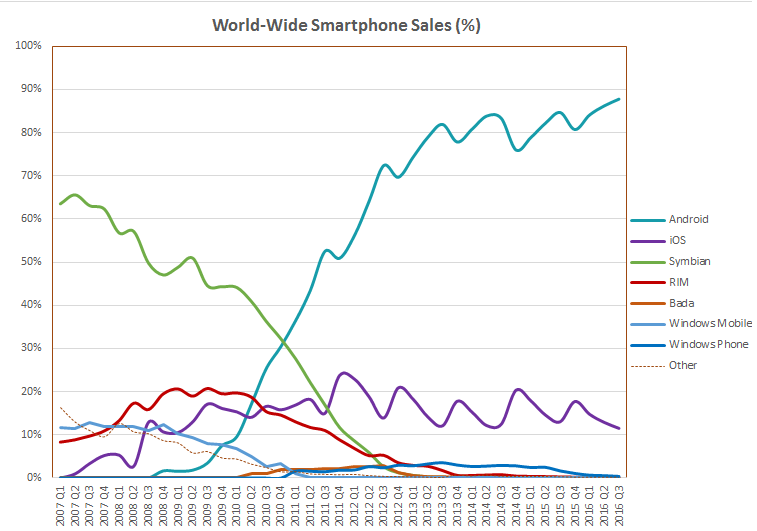
\includegraphics[width=0.8\textwidth]{Figures/World_Wide_Smartphone_Sales_Share.png}
\caption{World-wide smartphone sales \cite{wikiSmartphoneSales}}
\label{figure:wikiSmrtphoneSales}
\end{figure}

By the end of millennium, mobile phones were almost in every family in the western hemisphere \cite{worldBank}. However, they were still used mainly for telephony and sending SMS, with occasional MMS in the first years of 2000s. There were only few devices, which tried to combine mobile phones with PDAs - small personal computers, targeted mainly for business and enterprise environments. They were running on operating systems such as Palm OS, BlackBerry OS and Windows CE, which later evolved into smartphone operating systems.

These hybrids of mobile phones and PDAs were the first predecessors of today’s smartphones. Probably, the most known series are Nokia 9000 Communicator devices. In 2000, Ericsson released E380, which was the first device marketed as “smartphone”. It was also the first device running Symbian OS, the dominant mobile operating system until 2010.

Several other companies have seen the potential of these hybrid devices, which combined mobility, telephony, computing power and allowed connection to the ever-growing Internet. Soon, Symbian, Palm, BlackBerry and Windows Mobile got new rivals. It was iOS in 2007, Android in 2008 and Bada in 2009. These new players shattered the mobile market - and two of them even surpassed the old operating systems. 

Today, the situation is very different than it was ten years ago. Symbian OS, Palm OS and Bada are all discontinued projects. BlackBerry OS (known as RIM) is at the brink of existence. Windows Mobile was replaced by Windows Phone, but has lost a large portion of the market. The dominant roles are held by iOS and Android.

\subsection{Current situation}
Specifying, which operating systems are relevant to our methodology is not a trivial task, if we want the methodology to be accurate also for years to come. Yet, there are several factors, which may help us determine the trends to come:
\begin{enumerate}
	\item Is the OS still officially supported?
	\item What is the current market share of active users?
	\item What are the market shares of the sales?
	\item What are the revenues for developing applications for a particular OS?
	\item How many developers support the OS?
\end{enumerate}
Answering these questions will help us assign priority to individual smartphone platforms. 

\subsection{Supported operating systems}
As of the August 2016, the following smartphone operating systems are still being developed and supported: 
\begin{itemize}
	\item Android (with multiple modifications, such as Cyanogen, Fire OS or MIUI)
	\item BlackBerry 10 (RIM OS)
	\item Firefox OS
	\item H5OS
	\item iOS
	\item Sailfish OS
	\item Tizen
	\item Ubuntu Touch OS
	\item Windows 10 Mobile (previously Windows Phone 8.1)
\end{itemize}

\subsection{Smartphone OS usage market share}
Table \ref{table:phonemarketshare} shows the percentage of smartphone users for each smartphone OS (for the year 2016) \cite{mosMarketShare}.

\begin{table}[hb]
	\centering
	\caption{Smartphone OS usage market share}
	\label{table:phonemarketshare}
	\begin{tabular}{l r r}
		\toprule		
		Platform & Market share (\%) & Devices (approximate, in millions) \\
		\midrule
		Android & 65.33\% & 1371.93 \\
		iOS & 27.8\% & 583.8 \\
		Windows & 2.64\% & 55.44 \\
		BlackBerry & 1.18\% & 24.78 \\
		Symbian & 1.15\% & 24.15\\
		Other & 1.9\% & 39.9\\
		\midrule
	\end{tabular}
\end{table}

The approximate number of active devices is based on the figure that there is about 2.1 billion smartphones in use worldwide \cite{noOfSmartphones}. With more than a billion active devices, Android is clearly the most used mobile operating system. iOS is also very strong, having more than a quarter of the market share. The other platforms are far behind. Windows users are just a tenth compared to Apple’s iPhone and iPad users. The portion BlackBerry’s RIM users is just slightly above 1\%. Symbian, having a similar share although being discontinued, is still used by more than 20 million users.

\subsection{Smartphone OS sales market share}
The smartphone sales market share can help us predict the future growth or decline of a certain platform. As seen in Figure \ref{figure:wikiSmrtphoneSales} earlier in this chapter, there was a dramatic shift in 2010 and 2011, when Android surpassed Symbian in the percentage of sold smartphones.

\begin{table}
	\centering
	\caption{Smartphone OS sales, various reports from \cite{gartner}}
	\begin{tabular}{l l l l l l l l}
		\toprule
		Year & RIM & Symbian & iOS & Android & Bada & Windows & Other\\
		\midrule		
		2016 & 0.19\% & - & 14.78\% & 84.1\% & - & 0.7\% & 0.23\% \\
		2015 & 0.37\% & - & 16.26\% & 80.52\% & - & 2.47\% & 0.38\% \\
		2014 & 0.6\% & - & 15.4\% & 80.7\% & - & 2.8\% & 0.5\% \\
		2013 & 1.9\% & 0.1\% & 15.6\% & 78.4\% & 0.2\% & 3.2\% & 0.6\% \\
		2012 & 5\% & 4.2\% & 19.1\% & 66.4\% & 2.3\% & 2.5\% & 0.5\% \\
		2011 & 10.9\% & 18.74\% & 18.92\% & 46.53\% & 2.01\% & 1.65\% & 1.21\% \\
		\midrule		
	\end{tabular}
\end{table}

By the end of 2013, Symbian and Bada were pronounced discontinued. Windows Mobile transformed to Windows Phone in 2010. However, the transformation was not very successful. Windows Phone’s sales peaked at 3.2\% in 2013 and have been decreasing ever since. Compared to the 12\% market share of Windows Mobile in 2007, this situation looks very bleak for Microsoft. 

Even worse, however, are the numbers for another former major smartphone OS. BlackBerry’s RIM had almost 20\% market share in 2009. Now, for two years its sales have dropped below 1\%. iOS on the second place has its sales market share fluctuating around 15\%, but there is a large gap between the second and the first place. Android, now with stunning 84.1\% of all smartphone sales is the major force in the industry. 

Yet, the raw sales percentages may not necessarily correspond to the change of user base in absolute numbers. There is the possibility that Android users are buying new devices more often compared to iOS or Windows users, resulting in higher sales. But it definitely shows the trends whether a certain platform is experiencing its rise or fall.

For certain businesses, the global data may not be relevant, since regionally the sales percentages differ substantially.

\begin{table}
	\centering
	\caption{Regional smartphone sales in 2016}
	\label{table:regionalSmartphoneSales}
	\begin{tabular}{l l l l l l}
		\toprule
		\% & Android & BlackBerry & iOS & Windows & Other \\
		\midrule
		USA & 58.2 & 0.1 & 39.1 & 2.6 & 0 \\
		Mexico & 90.5 & 0.7 & 5 & 2.6 & 1.2 \\
		Brazil & 92.4 & 0 & 3.3 & 4.1 & 0.1 \\
		Argentina & 83.5 & 3.4 & 0.9 & 9.1 & 3.2 \\
		UK & 52.6 & 0.2 & 38.6 & 8.6 & 0 \\
		Germany & 74.2 & 0.6 & 19.3 & 5.9 & 0.1 \\
		France & 71.8 & 0.5 & 19.3 & 7.8 & 0.5 \\
		Spain & 87.8 & 0 & 11.4 & 0.8 & 0 \\
		Italy & 78.1 & 0.2 & 14.4 & 7.2 & 0.1\\
		Russia & 71.2 & 0.6 & 14.8 & 10.6 & 2.7 \\
		China & 73.9 & 0 & 25 & 0.9 & 0.3 \\
		Japan & 48.7 & 0 & 50.3 & 0.5 & 0.5 \\
		Australia & 52.6 & 0.2 & 41.2 & 5.4 & 0.6 \\
		World & 84.1 & 0.19 & 14.87 & 0.7 & 0.23 \\
		\midrule
	\end{tabular}
\end{table}

\begin{figure}
	\centering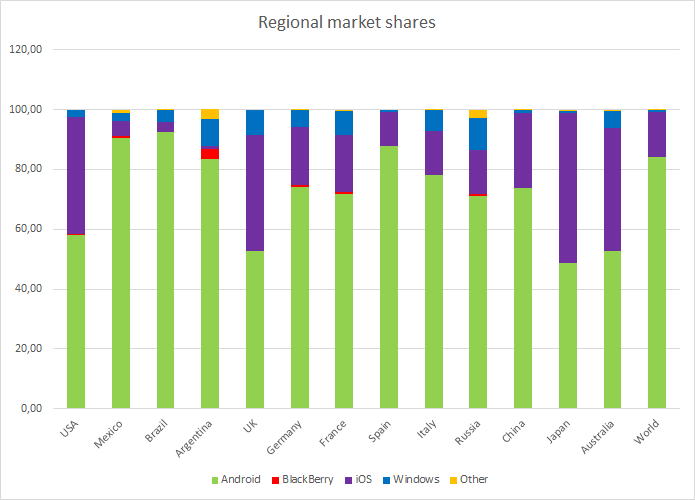
\includegraphics[width=0.8\textwidth]{Figures/regionalMarketShares.png}
	\caption{Regional market shares \cite{kantarOSSales}}
	\label{figure:regionalMarketShares}
\end{figure}

\subsection{Smartphone app stores revenues}
The sheer numbers of mobile platform users or device sales is one thing. But many developers - and almost all businesses - are motivated by something else entirely. Money may be a very decisive factor in choosing, which platforms will be targeted and which will be omitted. 

For some time now, it is common knowledge that Android users are not as willing to pay for apps as their iOS colleagues \cite{iosUsersPay}. This has been true also in recent years. Although the number of downloaded apps in Google Play is twice as high compared to Apple’s App Store, iOS is creating 70\% more revenue compared to Android \cite{iosAndroidStore}. 

These data are backed also by a survey performed by InMobi \cite{lifehackerRevenues}. While on average an Android developer\footnote{The survey does not distinguish between individual developers, developer groups or companies - all three are represented by the term "developer"} makes \$4900 per month, an iOS developer earns \$8100. However, there is a much more interesting discovery made by the survey. Developers targeting Windows earn the most - on average \$11400 per month.

\begin{figure}
	\centering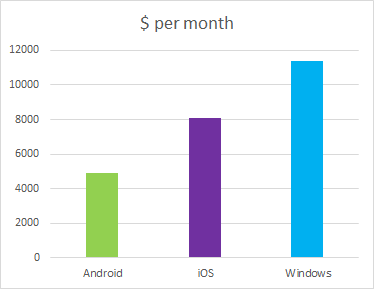
\includegraphics[width=0.5\textwidth]{Figures/appRevenues.png}
	\caption{Average app revenues from individual app stores, per month}
	\label{figure:appRevenues}
\end{figure}

The article explains this by the small amount of apps found on Windows Store. Smaller market means less competition and this has dual effect on the market. The discoverability factor of your application is much higher and the chance there will be a free alternative is much smaller. With no competition, a developer is free to increase the cost of an application \cite{appsInStores}.

\begin{figure}
	\centering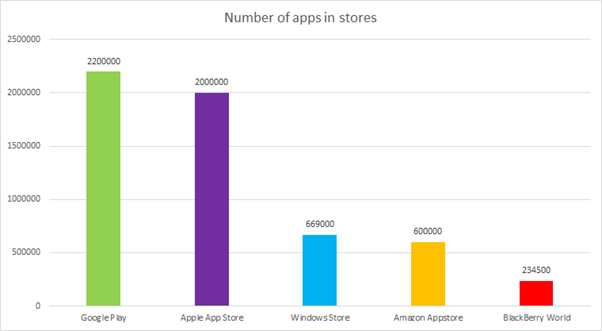
\includegraphics[width=0.8\textwidth]{Figures/appsInStores.png}
	\caption{Estimated number of apps in individual app stores.}
	\label{figure:appsInStoress}
\end{figure}

However, some \cite{betanewsWinRevenue} suggest the survey numbers may be skewed due to smaller sample of Windows developers. Even if the Windows monthly revenue is not accurate, the numbers make it still a very interesting platform. This cannot be said of other platforms. From the ones not discontinued, BlackBerry is the strongest one. However, its revenues do not figure in many recent surveys. In older articles, BlackBerry app development seems to be the least rewarding \cite{bgrBBRevenues}. 

\subsection{Operating systems targeted by developers}
There is one more factor that may decide about the future of a mobile operating system, and that is the number of developers creating new apps. A rich and healthy application store environment may help to attract new customers. 

As we have seen in figure 4, both Google Play and Apple App Store are very rich application markets. The numbers exceeding 2 million may even be discouraging for some developers, since they present both low discoverability and high competition. This can be vastly different in Windows and Amazon Stores, where the numbers are smaller by 2/3. For BlackBerry, the number is even smaller. And unlike other stores, BlackBerry World does not seem to grow with a comparable rate \cite{wikiBBWorld}. 

So, how many developers create apps for the individual operating systems? According to VisionMobile \cite{devEconomics} more than two thirds develop for Android. About one half creates applications for iOS and only one quarter for Windows.

\begin{table}
	\centering
	\caption{Portion of developers creating apps for individual operating systems}
	\begin{tabular}{l l l l l}
		\toprule
		 & Q1 2014 & Q3 2014 & Q1 2015 & Q3 2015 \\
		\midrule
		Android & 71\% & 70\% & 71\% & 71\% \\
		BlackBerry & 14\% & 11\% & 13\% & unavailable \\
		iOS & 55\% & 51\% & 54\% & 51\% \\
		Windows & 26\% & 28\% & 30\% & 27\% \\
		\midrule
	\end{tabular}
\end{table}

As it seems, part of developers is slowly abandoning the mobile web apps development and choosing one of the three dominant platforms as their primary. It is interesting that the number of developers having Windows as their primary platform is almost the same as the number of developers targeting Windows exclusively. And even though there is much more developers creating apps for Android compared to iOS, the number of developers claiming both operating systems as their primary is roughly the same.

\begin{table}
	\centering
	\caption{Primary platform for individual developers}
	\begin{tabular}{l l l l l}		
		\toprule
		 & Q1 2014 & Q3 2014 & Q1 2015 & Q1 2016 \\
		\midrule
		Android & 35\% & 40\% & 40\% & 41\% \\
		BlackBerry & 3\% & 2\% & 2\% & 1\% \\
		iOS & 38\% & 38\% & 37\% & 39\% \\
		Windows & 4\% & 7\% & 8\% & 9\% \\
		Web \& others & 20\% & 13\% & 13\% & 11\% \\
		\midrule
	\end{tabular}
\end{table}

\begin{table}
	\centering
	\caption{Developers creating apps exclusively for particular OS}
	\begin{tabular}{l l l}
		\toprule
		Android & iOS & Windows \\
		\midrule
		28\% & 12\% & 8\% \\
		\midrule
	\end{tabular}
\end{table}

When put in relation with the market shares and revenues, we can get some interesting data. Although Apple App Store is producing 70\% more revenue than Google, only 12\% developers create iOS exclusive apps, compared to 28\% Android exclusives. Android beats iOS also in the number of developers picking it as primary platform and overall number of developers. It does not seem probable that developers and IT companies would favor a larger user base, which produces smaller profit. However, there might be other factors discouraging developers from targeting iOS:
\begin{itemize}
	\item ObjectiveC is more complex and difficult to learn, compared to Java (this might change with the introduction of Swift)
	\item iOS can be built only on MacOS devices (Android apps can be developed on MacOS, Windows and Linux)
	\item Publishing apps on Apple App Store is more complex and expensive compared to publishing on Google Play
\end{itemize}

Another interesting pair to compare is BlackBerry and Windows. Both have small user bases and low sales. But while BlackBerry has small revenues and only 1\% of developers targeting it as primary platform, Windows has the highest revenues and 9\% of developers targeting it as primary platform and 27\% developing also Windows apps. This can be seen also on their app stores - Windows Store has 3-times more applications than BlackBerry World and is still growing, while the latter stagnates for several years. With Windows 10 unifying the development for desktop, tablet and mobile, the numbers can grow even faster and eventually, it might be the developers who will save the Windows mobile platform.

\subsection{Tablets}
So far the thesis has been concerned mainly by smartphones. Yet, there is another major group of mobile devices - tablets. In the current market, the lines between individual device categories is often blurred. Between smartphones and tablets there are phablets and the gray zone between tablets and notebooks is composed of netbooks, ultrabooks and tablets with detachable keyboard. Moreover, with the introduction of Continuum for Windows \cite{microsoftContinuum}, it is hard to tell whether there is a border at all.

Yet, the development environment for iOS distinguishes between apps for iPhone and iPad \cite{appcodaiPad} and also Android has special guidelines for adjusting apps for tablets \cite{androidTablet}. Therefore, let us take a look at the OS market shares of tablets as well.

\begin{table}
	\centering
	\caption{Global market share of tablet operating systems \cite{tabletMarketShare}}
	\begin{tabular}{l l l l l}		
		\toprule
		 & 2013 & 2014 & 2015 & 2016 \\
		\midrule
		Android & 62.36\% & 67.33\% & 67.4\% & 66.2\% \\
		iOS & 33.93\% & 27.57\% & 23.9\% & 22.4\% \\
		Windows & 3.5\% & 5.09\% & 8.6\% & 11.3\% \\
		\midrule
	\end{tabular}
\end{table}

Inferring from smartphone market shares, it is no surprise that Android is the most used operating system, followed by iOS and Windows respectively. BlackBerry PlayBook does not figure in the statistics at all. However, very interesting is Windows on tablets compared to smartphones. While the Windows smartphone share was below 3\% and decreasing, in tablet world Windows is on the rise. It is estimated, that by 2020 Windows will have almost 20\% of the market share, similar to iPads \cite{idcTabletShare}. Already now, Windows is the dominant operating system, when it comes to 2in1 devices, like detachable tablets \cite{idcDetachableTablets}. With the introduction of the Windows universal platform development paradigm, Windows starts to be supported also by tools, which had not taken it into consideration before \cite{codenameOneNaive}. 

\subsection{Conclusion}
Based on the previous factors, we can filter out three mobile operating systems, which will be relevant to our methodology - Android, iOS and Windows. The support of two of them - Android and iOS - will be a crucial factor, when selecting suitable development tools. 

Android has clearly the largest market share, both for smartphones and tablets. With the exception of Japan, it has also the highest sales, biggest app store and is targeted by the largest portion of developers. iOS has less than a half of Android’s smartphone market share, and even smaller numbers for tablets and future sales. Still, it takes up 1/4 of the market, is targeted by more than half of the developers and Apple App Store has 70\% higher revenues than Google Play.

Windows is a debatable operating system. In smartphone world, it has low market share and sales below 1\%. However, it has the highest relative revenues, has growing tablet market share and more than 25\% developers create apps for Windows Store as well. Moreover, around 36\% of multi-platform tool users wish their tool to support Windows development as well \cite{cptBenchmarking2014}. Therefore, we will not omit development tools that do not support Windows. Yet, for those that do, we will compare Android and iOS capabilities with Windows as well.

There are two more operating systems - BlackBerry and Symbian - that have around 1\% share of smartphone users. Although these OSs may be interesting for some niche markets, the thesis will not consider them as primary points of interest. Symbian is a discontinued project and BlackBerry seems to be transforming into a hardware company, producing Android devices. Occasionally, these platforms may be referred in relation with individual multi-platform development tools.



\section{Mobile multi-platform development tools}
For each software platform there exists one or two official tools, languages, APIs and supporting software making up a development stack. And then there exists a ton of various modifications, customizations, frameworks and corporate tools to enhance and speed up the development for a narrow range of implementation problems.

The same is true for mobile development. The official development tools \cite{taxonomyCP} can be found in table \ref{table:officialDevelopmentTools}.
\begin{table}[!ht]
	\centering
	\caption{Official mobile OS development tools}
	\label{table:officialDevelopmentTools}
	\begin{tabular}{p{2cm} p{2cm} p{2cm} p{2.5cm} p{2.5cm} p{2.5cm}}
		\toprule
		Platform & IDE & Language & User interface & Desktop development & App market\\
		\midrule
		Android & Android Studio & Java & XML & Linux, macOS, Windows & Google Play\\
		BlackBerry (RIM) & Momentics & C++ & Qt \& QML & Linux, macOS, Windows & BlackBerry World \\
		iOS & XCode & ObjectiveC & ObjectiveC or Cocoa Pods & macOS & Apple iTunes \\
		Windows & Visual Studio & C\# & XAML & Windows & Windows Store \\
		\midrule
	\end{tabular}
\end{table}

That were the official tools, initially created by the owner companies to enable developers create apps for their respective platforms. But already now, things start to get complicated. You can create C++ apps also for Android and Windows. And, although you will need to implement an Objective C wrapper, you can create C++ libraries for iOS, as well.

It seems, we have found the perfect cross-platform tool. As the reader will learn later, C++ can really be used for cross-platform development, but it is not that straightforward. The C++ support for Android and iOS is limited. And each platform has a different application lifecycle, different hardware peripheries, different APIs and libraries. In the end, developing in C++ would result in developing 4 different applications - but in a much more difficult way.

In the table \ref{table:officialDevelopmentTools}, there is one more language known for its “multiplatformicity” - Java. However, its “Write once, run anywhere” is not so true in the mobile world. While BlackBerry was forced by its declining market share to support Android apps written in Java, iOS and Windows are not so supportive. Yet, even for Java there are tools which enable it to spread even to those platforms. So, let us discover those cross-platform development options up close.

\subsection{Multi-platform development approaches}
As we have seen above, there is no common development tool for all mobile platforms. Even if we ignored the differences in programming languages, there are still various paradigms in application lifecycle, access to native APIs, interactions between processes, etc.

For many companies - or individual developers - it is too expensive to have an expert for each platform and each language. They have to struggle, to either omit certain platform, or learn new skills for each OS. However, certain aspects of every mobile application can be abstracted and standardized. And this is where multi platform development tools come into play. They take a single language, single development tools and abstract application aspects across all mobile operating systems to create a unified code based. The level of abstraction is a crucial factor which can help us differentiate between individual multiplatform tools. If the level of abstraction is high, we get a “Write once, run anywhere” approach, but lose the control over the specifics of individual platforms. If the level of abstraction is lower, we can access the platform specific features, but we have to implement them individually and the shared code base is smaller.

There exist multiple ways how to divide and categorize multi-platform development tools. Research2guidance \cite{cptBenchmarking2014} classifies multi-platform tools according to how the app is created into following classes: Web app toolkits, App factories, Cross-platform integrated development environments, Cross-platform integrated development environments for Enterprise, Cross-platform compilers, Cross-platform services. Silva’s division \cite{ribeiroDaSilva} is a bit different: App factory, Web-to-native wrapper, Runtime and Domain-specific language.

Probably the best known division is into following 3 categories \cite{aComparativeStudy} \cite{smutny} \cite{taxonomyCP}:
\begin{itemize}
	\item Native apps - mobile applications that are installed on the device, executed by the OS and have full access to native APIs and sensors.
	\item Web apps - HTML, CSS and JavaScript web apps accessed from the mobile browser. They do not have to be installed, but have no access to native APIs or sensors (with the exception of camera and file system).
	\item Hybrid apps - web apps that are bundled within a customized web view container. Through this web container they are able to access the native APIs and sensors. The app has to be installed, but provides all benefits of a web app.
\end{itemize}

However, this categorization does not distinguish between truly native approach and tools that mimic native behaviour with custom runtimes, virtual machines or cross-compilation \cite{definingTelerik}. Therefore, this thesis uses following categories: mobile web apps, hybrid apps, interpreted apps and cross-compiled apps. \cite{uppsala}\cite{rajTolety}\cite{evaluationOfCP}. In \cite{aarhus}, Nielsen introduces a fifth approach - source translation, or transpiling. However, this last approach is usually used in combination with one of the previous approaches.

\subsubsection{Mobile web apps}
It is often stated by many developers, that the only true multi platform development is possible only via standard web technologies - HTML, CSS and JavaScript. It is true that all smartphones have a web browser capable of displaying web pages and apps. Mobile web apps are exactly that - classic web apps adapted for a mobile browser. However, each browser can render the web app in a different manner, resulting in inconsistent user experience. Moreover, the application can be slow, depending on the connection speed and browser interpretation capabilities. Plus, there is very restricted, or no connection to the native APIs and hardware tools.

\subsubsection{Hybrid applications}
Hybrid apps try to minimize the problems of web apps, while benefiting from their strengths. They wrap the JavaScript (and HTML + CSS) application in a lightweight native wrapper, most often a webview stripped of almost all functionality. Unlike mobile web apps, hybrid applications are available also offline and have much better access to native APIs, interfaces and peripheries. However, the native functionality may differ for each OS. The application is still in a web browser, which drastically decreases its performance. Plus, the nature of JavaScript does not allow to use multiple threads. Also, hybrid applications do not have access to native UI. A drawback for some may be a benefit to others - the application will look the same on each operating system. 

\subsubsection{Interpretation}
Interpreted apps utilize a custom runtime environment or virtual machine (like JavaScript engine or Java Virtual Machine), while interfacing with the native platform at the same time. Interpreted apps are written predominantely in JavaScript, similar to mobile web apps and hybrid apps. However, they are not executed in a web browser, so there is no sand-box limitation and no HTML DOM. As the name suggests, the code is directly interpreted by an included JavaScript engine. Access to native APIs and sensors is almost unlimited. Various tools provide various UI rendering techniques - some use native UI elements (like Appcelerator and NativeScript), others provide a platform-agnostic unified UI (e.g. Codename One and React Native). Performance-wise, interpreted apps are in between hybrid and cross-compiled apps. However, they allow faster protoryping process, since updating code does not require a build process.

\subsubsection{Cross-compilation}
To the developer, creating a cross-compilation or interpreted application may seem very similar. However, cross-compilation is a much more complicated process. 
Cross-compilation describes the practice of developing an app using platform-agnostic API or programming language. The cross-compiler transforms the code into native platform-specific executable apps (or libraries). While some tools (e.g. Kivy or Qt) apply this process to all layers - from data layer to UI - resulting in a true WORA approach, others allow more platform-specific access (like RubyMotion or Xamarin). Cross-compiled apps have performance closest to truly native apps. Due to complicated process of cross-compilation and OS differences, some tools combine cross-compilation with interpretation (e.g. Mono.Android interprets code from .NET libraries).

\subsubsection{Source translation}
The last approach, source translation is based in translating one high-level programming language into another. The app is then run from the platform-specific programming language. Similar to cross-compilation and Virtual Machines, the advantages of this technique is the native performance, native UI and almost unlimited access to native API. However, no framework uses pure source translation approach. Rather, it is combined with other approaches - hybrid, interpreted or cross-compiled - where only part of code is translated.

\subsection{MBaaS}
For many businesses the use case of an internal company application is often the same - to collect inputs, store them, and to perform various analyses, display data and notify employees when necessary. This requires a database server, or other cloud storage, web api, web server, and often both a mobile and web application. To implement the complete work flow correctly and efficiently a whole group of software engineers, developers and coders is needed. Many companies would need to outsource development of such project, or hire several freelance developers. Further costs connected with support services and the need to reveal company secrets to 3rd parties are all risks that many are not willing to undertake.

For these purposes, complex solutions known as Mobile Backend as a Service (MBaaS) began to emerge. An MBaaS allows the design and development of a database, web api, mobile and web app in a single tool. These tools often provide visual programming, with occasional customization of code in JavaScript, or another scripting language. 

Depending on the MBaaS provider, some tools allow integration with an existing backend, creating only a bridge to the client application and adding integration to social networks. The mobile applications created with an MBaaS are usually mobile web apps or hybrid apps. Most MBaaS services are commercial, with limited open source support.

\subsection{Multi-platform development frameworks and tools}
As mentioned in earlier chapters, as of 2016, there exists more than a hundred different tools and services for mobile multi-platform development. A crucial factor of this thesis, however, is the focus on native API usage. Thus, a lot of these tools are not relevant for further discussion. Here is the list of all criteria that a tool must pass in order to be investigated further. Each criterion contains a short description, why is it important, and a few examples of tools that did not pass.
\begin{enumerate}
	\item \textbf{The tool is not discontinued.}
	For obvious reasons, only frameworks and platforms that are still supported and developed will be considered. A discontinued project may be interesting for experimental purposes, but its use in production is highly unlikely, and questionable.
	Examples: MoSync, RoboVM, WidgetPad
	\item \textbf{At least Android and iOS are supported.}
	Since Android and iOS are the two dominant players in the smartphone world, any multi-platform tool must support at least these two operating systems. The support for Windows is advantageous, but optional. 
	Examples: AML, Appinventor, Java ME, Kallipso
	\item \textbf{The tool is not game-centric.}
	Many game frameworks work seamlessly across multiple operating systems. However, they neither intend, nor are able to use the native interfaces.
	Examples: Marmelade, Unity, Wave
	\item \textbf{General app development is possible.}
	This may be considered an extension of the previous criterion. The tools must allow development of almost any kind of mobile application. All tools bound to a particular business will be rejected. This includes also all MBaaS solutions which do not allow server-less implementation of mobile application.
	Examples: appMobi (mobile security), Appticles (publishing), i-exceed (banking), Pegasystems (customer engagement), and rejected MBaaS tools (AnyPresence, AppGyver, Kinvey, Mobile Frame, MooFWD)
	\item \textbf{The tool must allow access to most used native APIs.}
	Access to the camera, GPS, accelerometer, gyroscope, media, file system and local database must be granted. This criterion eliminates all mobile web app frameworks, since their access is limited by the rendering browser.
	Examples: AppPress, Dojo, Bootstrap Mobile, jQuery Mobile, Sencha Touch
\end{enumerate}

The complete table of all mobile multi-platform development tools which passed all criteria can be found in table \ref{table:frameworks}. Out of more than 100 tools, only 25 fulfilled all necessary criteria. More information about the rejected tools can be found in \cite{aarhus}. 

\begin{sidewaystable}
	\centering
	\caption{Selected multi-platform development tools}
	\label{table:frameworks}
	\begin{tabular}{l l l r r r r}
		\toprule
		Product & Language & Approach & MBaaS & Apache Cordova & Windows & BlackBerry \\
		\midrule
		Alpha Anywhere & Code-free, JavaScript & Hybrid & Yes & Yes & No & No \\
		Appcelerator & JavaScript & Interpreted & Yes & No & Yes & No \\
		Appery.io & Code-free, JavaScript & Hybrid, Web apps & Yes & Yes & Yes & No \\
		Aquro & JavaScript & Hybrid & Yes & Yes & No & No \\
		Codename One & Java & Interpreted & No & No & Yes & Yes \\
		Corona Labs & Lua & Cross-compiled & No & No & Yes & No \\
		Embarcadero & C++, Delphi & Cross-compiled, Web apps & No & No & Yes & Partially \\
		Fuse & JavaScript & Interpreted & No & No & No & No \\
		Instant Developer & Code-free, C\#, Java & Hybrid & Yes & No & Yes & No \\
		Ionic & AngularJS, JavaScript & Hybrid & No & Yes & Yes & Unofficial support \\
		Kivy & Python & Cross-compiled, Hybrid & No & No & Yes & No \\
		Kony & Code-free, JavaScript & Interpreted, Web apps & Yes & No & Yes & Only web apps \\
		Monaca & JavaScript & Hybrid & Yes & Yes & Yes & No \\
		NativeScript & AngularJS, JavaScript & Interpreted & No & No & Early access & No \\
		NeoMAD & Java & Cross-compiled & No & No & Yes & Yes \\
		NS Basic & BASIC, JavaScript & Hybrid & No & Yes & Only as web app & No \\
		PhoneGap & JavaScript & Hybrid & No & Yes & Yes & Yes \\
		Qt & C++ & Cross-compiled & No & No & Yes & Yes \\
		React Native & ReactJS, JavaScript & Interpreted & No & No & Planned & No \\
		RubyMotion & Ruby & Cross-compiled & No & No & No & No \\
		Smartface & Code-free, JavaScript & Interpreted & Partially & No & No & No \\
		Tabris.js & JavaScript & Interpreted & No & Yes & Yes & No \\
		Telerik Platform & AngularJS, JavaScript & Hybrid, Web apps & No & Yes & Yes & No \\
		ViziApps & Code-free, JavaScript & Hybrid, Web apps & Partially & No & No & No \\
		Xamarin & C\# & Cross-compiled & No & No & Yes & No \\
		\midrule
	\end{tabular}
\end{sidewaystable}

As the reader can see, the table still feature several development tools using the web application approach, altough it was said, those tools will be removed. This is due to the fact that some frameworks allow the developers to create various output applications, e.g. both hybrid and web apps.

Some MBaaS providers allow creating offline apps - their tools have been added to the table. They can be easily distinguished by the word "yes" in the MBaaS column. Similarly, all tools based or supporting Apache Cordova builds and plugins have the word "yes" in the Cordova column.

Naturally, all tools support app development for Android and iOS. It is worth noting that more than a half supports also Windows mobile development, with 3 more planning to do so in the near future \cite{codenameOneWinSupport} \cite{nativeScriptWinSupport} \cite{reactNativeWinSupport}. BlackBerry support is much sparses, with only 4 tools fully supporting RIM builds. 3 others have partial or unofficial BlackBerry support.

It is clear that the most popular programming language is JavaScript. Most tools take either hybrid or interpreted approach. Only a handful of them are cross-compiled.



\section{Development tools evaluation}
Already now we are able to distinguish several decisive criteria to choose a development tool for multi-platform mobile applications. The supported operating systems, programming languages, price, licencing, etc. However, to determine also other criteria, not visible on the first sight, further investigation needs to be done. We will pick a few development tools from previous chapter for evaluation and implement several use cases in them.

\subsection{Development tools chosen for evaluation}
To test the differences between individual tools, the most popular tool\footnote{According to a joint popularity index from Google Trends and G2Crowd} from each build approach was chosen. Xamarin, representing the cross-compiled group, serves as a reference framework, due to author’s previous experience with it. The largest group, hybrid apps, will be represented by its most known member - Apache Cordova. From tools using interpretation, React Native is on the rise.

\subsubsection{Xamarin}
Xamarin is a software company producing a mobile multi-platform development tool of the same name. It was established in May 2011 and acquired by Microsoft in February 2016. Xamarin (the platform) allows developers to code in C\# for Android, iOS and Windows. Developers can use the Visual Studio IDE on Windows or Xamarin Studio on both Windows and MacOS. However, only Android applications can be built on both operating systems. To create an iOS application, developer needs a Mac device to perform the build. Likewise, Windows (Phone) app can be developed only on a Windows (Desktop) machine. 

On iOS, Xamarin compiles Ahead-of-Time to native assembly, while on Android there is an intermediate compilation to IL code \cite{xamarin}. There are in fact two ways an application can be created. The classical approach allows sharing common business logic in a PCL (Portable Class Library - a C\# library for multiple platforms). However, the individual user interfaces and platform-specific behaviour has to be implemented for each platform individually. 

The second way to develop applications for Xamarin is via Xamarin.Forms. This is a custom-made UI framework, that removes the need to implement user interfaces for each platform individually. However, creating platform-specific behaviour is still possible (and in some cases required). With Xamarin.Forms the amount of code shared across platforms can be up to 100\% \cite{xamarin}.

\subsubsection{Apache Cordova}
One of the most popular multiplatform development tools is definitely PhonGap. PhoneGap is the original and most popular distribution of Apache Cordova \cite{apacheCordova}, which is an open source development framework enabling app development using HTML 5, CSS 3 and JavaScript. Cordova provides a native wrapper with a web view (or equivalent component) and accesses hardware peripheries with JavaScript API. The application itself is built within the web view wrapper. This type of app development is called hybrid. 

Although the application is installed natively and runs offline, the UI elements are often different, access to native API is restricted and the application tends to have decreased performance. Plus, for hackers and copycats it is very easy to download the installation package and extract the JavaScript files, since they are generally included as standard web content \cite{cordovaVsCodename}. 

Yet, developing using Apache Cordova (and other hybrid tools) is very fast, and some obfuscation tools exist. It is worth noting that PhoneGap is not the only distribution of Apache Cordova. There are many others, like Ionic, allowing development in Angular, NSBasic, developed in Basic, or Telerik, which supports JavaScript, Angular and TypeScript.

For the evaluation, the Visual Studio distribution of Apache Cordova was chosen. By default, it offers development in HTML 5, CSS 3 and JavaScript or TypeScript. However, it contains also templates for Angular projects and is directly recommended by the Ionic framework \cite{ionicGetStarted}. 

\subsubsection{React Native}
React Native is a multi-platform development tool created by Facebook. It uses similar technology as ReactJS and converts it into Android and iOS apps. Support for Universal Windows Platform is on the way and there already exists a unofficial plugin for Windows development\cite{npmReactNativeWindows}.

Although interpreted frameworks may seem similar to hybrid tools due to the use of JavaScript, there is no WebView container and no HTML DOM. Interpreted tools use alternative approaches to UI representation: Appcelerator and NativeScript use XML, React Native utilizes JSX. Although some interpreted frameworks provide native look and feel for the UI layer, due to the nature of JSX, React Native renders a platform-agnostic UI resembling web pages. 

JavaScript interpreted approach has been present for a while, thanks to Appcelerator. However, only in recent years it got more traction with the declining popularity of PhoneGap and the rise of tools like Fuse, NativeScript, Tabris.js and, most prominently, React Native. The only interpreted framework tool studied in this thesis, which does not use JavaScript, is Codename One with its Java implementation.

\begin{table}[!h]
	\centering
	\caption{Apache Cordova - Persistent storage demonstration apps}
	\label{table:cordova2}
	\begin{tabular}{p{5cm} | p{5cm} | p{5cm} }
		\toprule		
		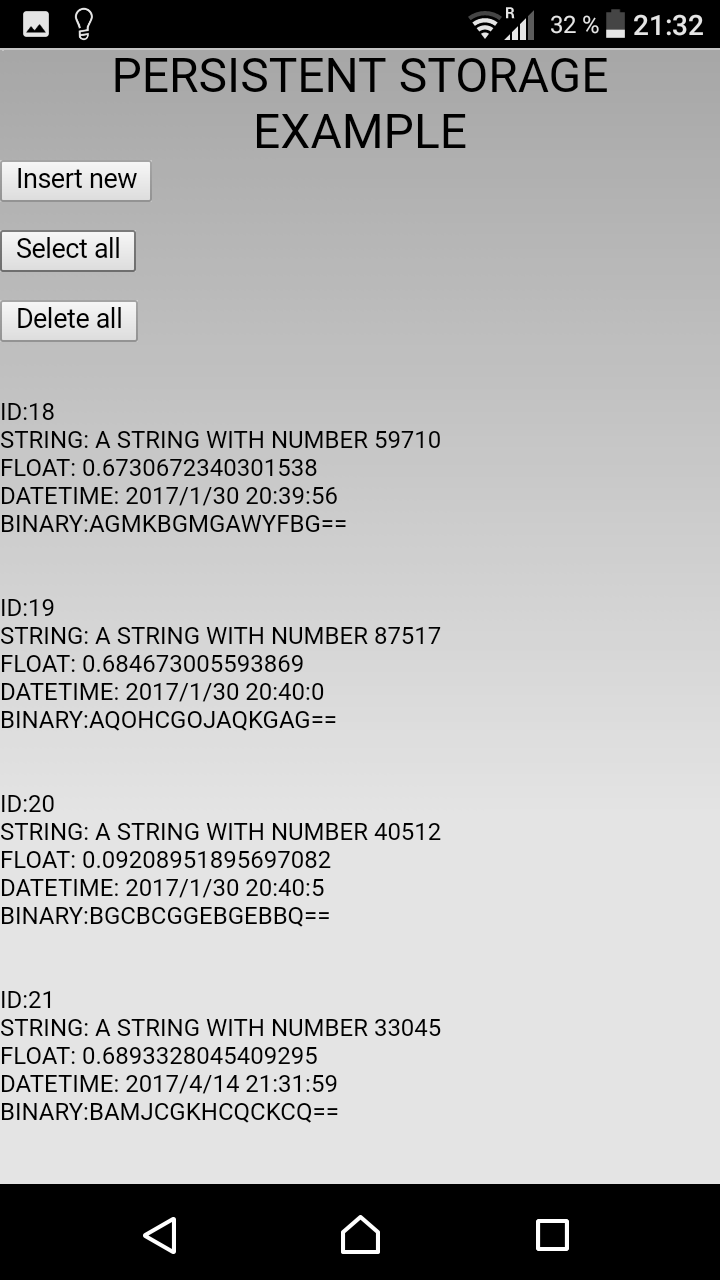
\includegraphics[width=0.3\textwidth]{Figures/cordova2android.PNG}
		& 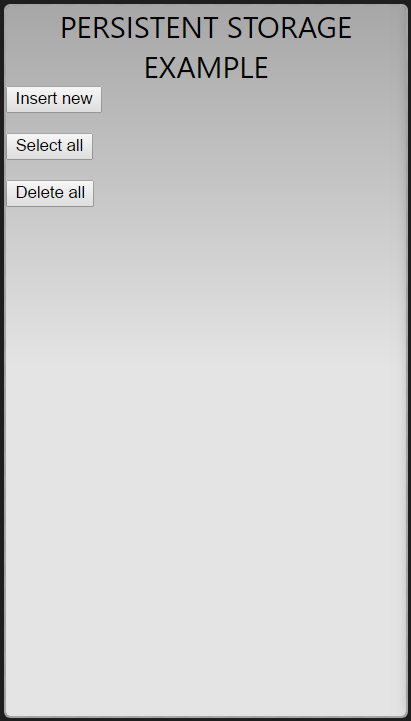
\includegraphics[width=0.3\textwidth]{Figures/cordova2ios.PNG}
		& 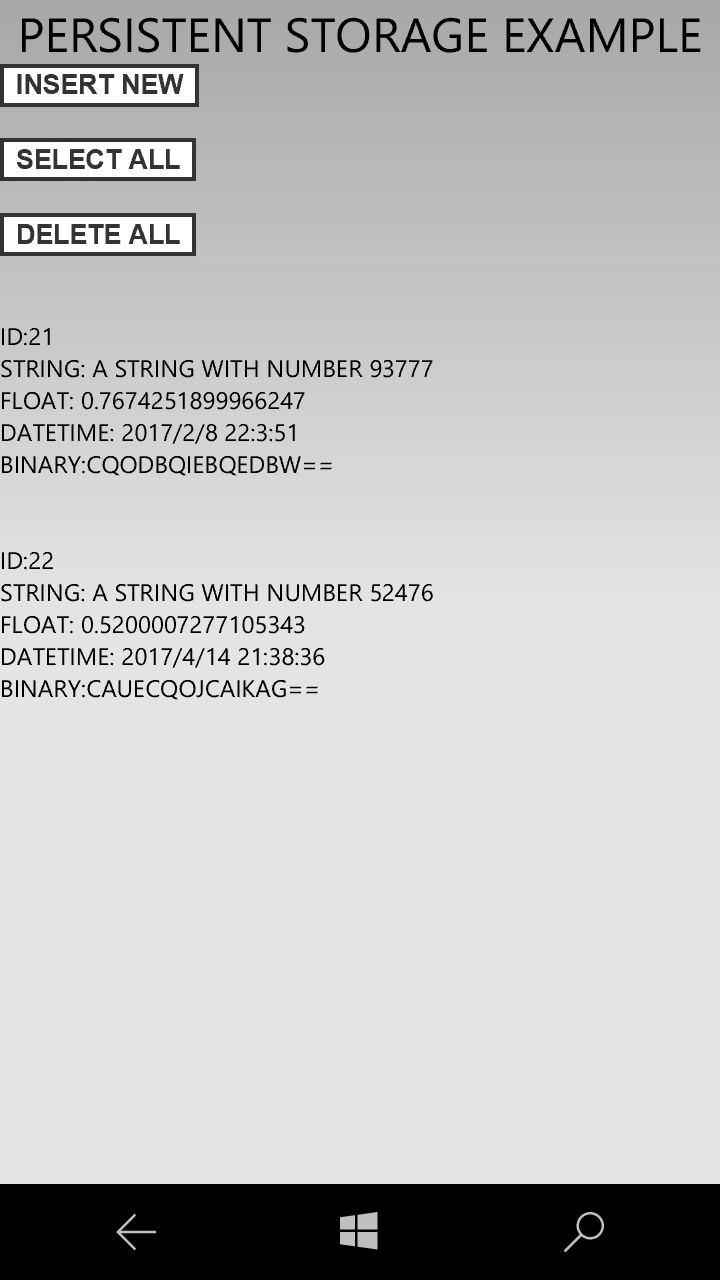
\includegraphics[width=0.3\textwidth]{Figures/cordova2windows.PNG}
		\\
		Android & iOS & Windows \\
		\midrule
	\end{tabular}
\end{table}

\subsection{Use case definition}
This is the list of use case scenarios, that will be implemented by each developer tool:

\begin{enumerate}
	\item \textbf{Hello world! }- the first scenario is the simplest one. The system will provide an almost blank application, with a single button. After clicking on the button, a “Hello world” text will be toggled.
	\item \textbf{Persistent storage }- this scenario will test the ability of the development tool to store and load data into a persistent storage. The following types will be stored: string, float, binary data and a more complex object.
	\item \textbf{Camera \& GPS }- the third scenario describes the most widely used hardware peripherals - camera and GPS. In this scenario, we will use the camera to take a photo and the GPS to add the coordinates of current location.
	\item \textbf{Custom UI element and using native code }- the next scenario explores the possibility of using a custom UI element. We will try to implement a circular progress bar. If there is the possibility to render a native element from the multi-platform framework directly, we will use that. Otherwise, we will call a native random number generator and then fill the circular progress bar to generated percentage.
	\item \textbf{Push notifications }- in the fifth scenario we will try to take advantage of the notification API of each platform. We will research the possibility to display push notifications sent from a web application. Because each platform handles the notifications differently, we will use only basic notifications without advanced features.
	\item \textbf{Tablet optimization} - the sixth use case will test the ability of the development framework or platform to adjust the UI elements for various screen sizes.
\end{enumerate}

Note, that the use cases cover only those aspects of multi-platform development, that can be achieved on all target operating systems (Android, iOS and Windows). Therefore, we will not test platform-specific features, such as fragments, widgets, life tiles, etc.

\begin{table}[!h]
	\centering
	\caption{Xamarin - Camera and GPS demonstration apps}
	\label{table:xamarin3}
	\begin{tabular}{p{5cm} | p{5cm} | p{5cm} }
		\toprule		
		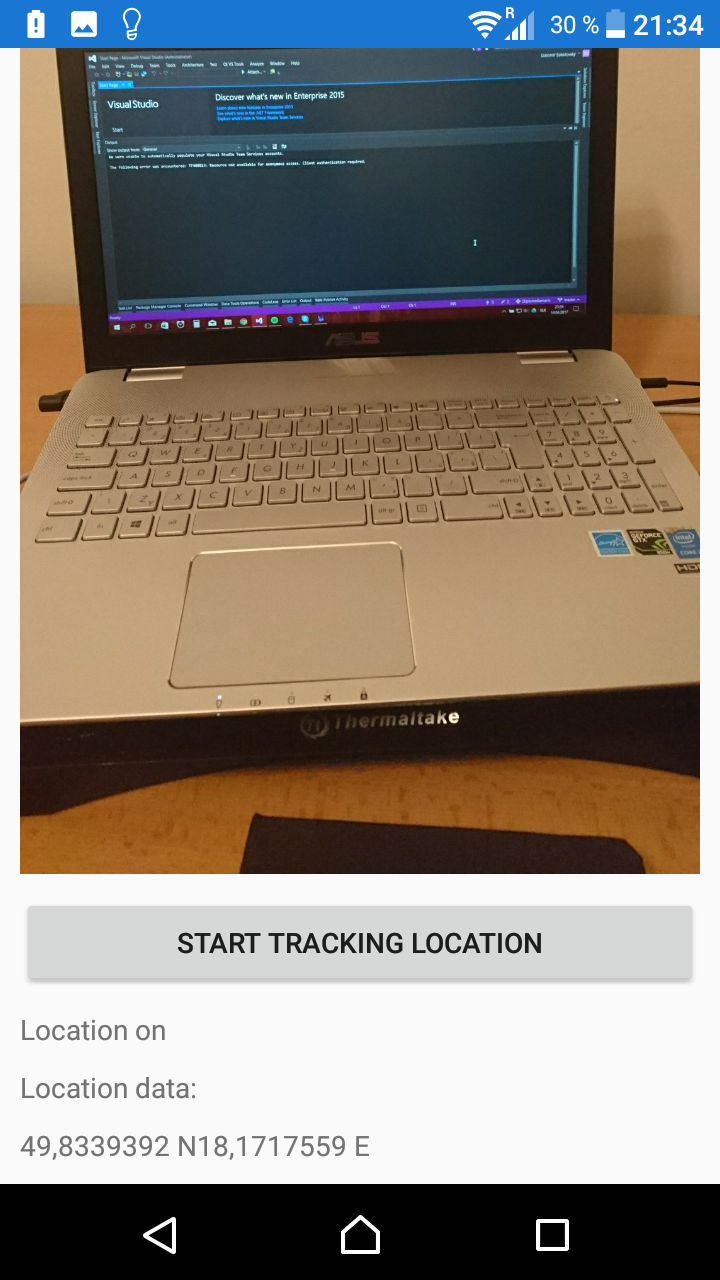
\includegraphics[width=0.3\textwidth]{Figures/xamarin3android.PNG}
		& 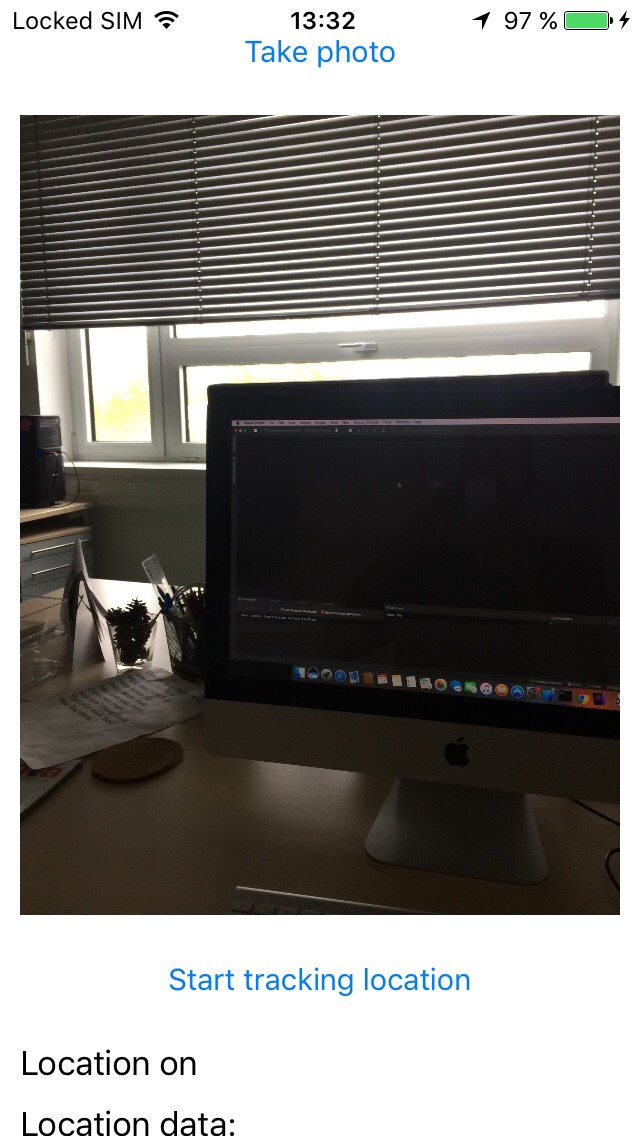
\includegraphics[width=0.3\textwidth]{Figures/xamarin3ios.jpg}
		& 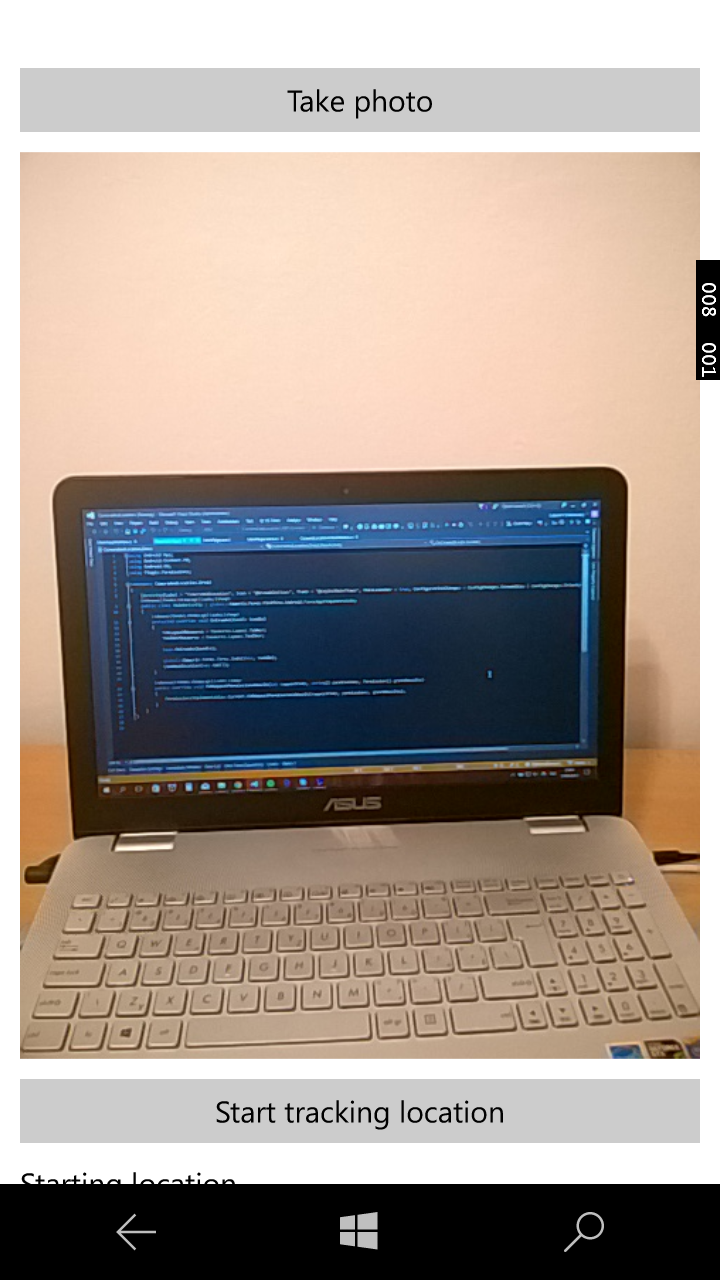
\includegraphics[width=0.3\textwidth]{Figures/xamarin3windows.PNG}
		\\
		Android & iOS & Windows \\
		\midrule
	\end{tabular}
\end{table}

\subsection{Hardware and software configuration}
The evaluation of development tools is performed on on a Windows machine for Android and Windows Phone. For iOS, the built (or whole development) is done on an iMac device. The specifications can be found in tables \ref{table:desktopConfiguration}, \ref{table:mobileConfiguration} and \ref{table:developmentToolsConfiguration}.

\begin{table}[!h]
	\centering
	\caption{Desktop configuration}
	\label{table:desktopConfiguration}
	\begin{tabular}{p{2cm} | p{4.5cm} p{4.5cm}}
		\toprule
		OS & Microsoft Windows 10 Home & macOS Sierra, v 10.12.3 \\
		Model & Asus N551J & iMac 21.5-inch, Mid 2011 \\
		Processor & Intel Core i7-4720HQ x64, 2.6 GHz & Intel Core i5, 2.5 GHz \\
		Memory & 16 GB & 16 GB \\
		Storage & 120 GB SSD, 950 GB HDD & 512 GB HDD \\
		\midrule
	\end{tabular}
\end{table}

\begin{table}[!h]
	\centering
	\caption{Mobile configuration}
	\label{table:mobileConfiguration}
	\begin{tabular}{p{2cm} | p{3.5cm} p{3.5cm} p{3.5cm}}
		\toprule
		OS & Android Marshmallow 6.0.1 & iOS 10 & Windows 10 Mobile \\
		Model & Sony Xperia Z5 Compat (E5823) & iPhone 5S & Nokia Lumia 735 \\
		Processor & Qualcomm Snapdragon 810, Octa-core x64, 2 GHz & Apple A7 chipset, Dual-core x64, 1.3 GHz & Qualcomm Snapdragon 400, Quad-core x64, 1.2 GHz \\
		Memory & 2048 MB & 1024 MB & 1024 MB \\
		Storage & 32 GB internal, 32 GB SD card & 16 GB internal & 16 GB internal, 16 GB SD card \\
		\midrule
	\end{tabular}
\end{table}

\begin{table}[!h]
	\centering
	\caption{Development tools configuration}
	\label{table:developmentToolsConfiguration}
	\begin{tabular}{l}
		\toprule
		\textbf{Xamarin}\\
		\midrule
		Microsoft Visual Studio Enterprise 2015, Update 3 \\
		Xamarin for Visual Studio 4.2, Xamarin.Android 7.0, Xamarin.iOS 10.0 \\
		Tools for Universal Windows Apps 14.0 \\
		\midrule
		\textbf{Apache Cordova}\\
		\midrule
		Microsoft Visual Studio Enterprise 2015, Update 3 \\
		Tools for Apache Cordova Update 10 \\
		Tools for Universal Windows Apps 14.0 \\
		Tools for Universal Windows Apps 14.0 \\
		\midrule
		\textbf{React Native}\\
		\midrule
		JetBrains WebStorm 2016.3 \\
		React Native v 0.41\\	
		\midrule	
	\end{tabular}
\end{table}

\subsection{Results}

This subsection summarizes the results of evaluated apps. Apache Cordova was implemented via Visual Studio plugin and tested on Android, iOS and Windows. The main development machine was Windows. No special architectural style or design patterns were used.

On the other hand, React Native was developed almost entirely on macOS in WebStorm. Although there exists a custom UWP plugin for React Native, running an app on Windows device was not achieved. Therefor, React Native was evaluated only on Android and iOS. For more complicated projects, the Redux architecture was used. 

Similar to Apache Cordova, Xamarin was also primarily developed on Windows desktop and tested on Android, iOS and Windows mobile. To get closer to the UI development experience of the other evaluated frameworks, Xamarin.Forms in combination with MVVM was chosen.

\begin{table}[!h]
	\centering
	\caption{4th use case in individual frameworks}
	\label{table:frameworks4}
	\begin{tabular}{p{3cm} | p{4cm} | p{4cm} | p{4cm} }
		\toprule			
		& Android & iOS & Windows \\
		\midrule
		Apache Cordova	
		& 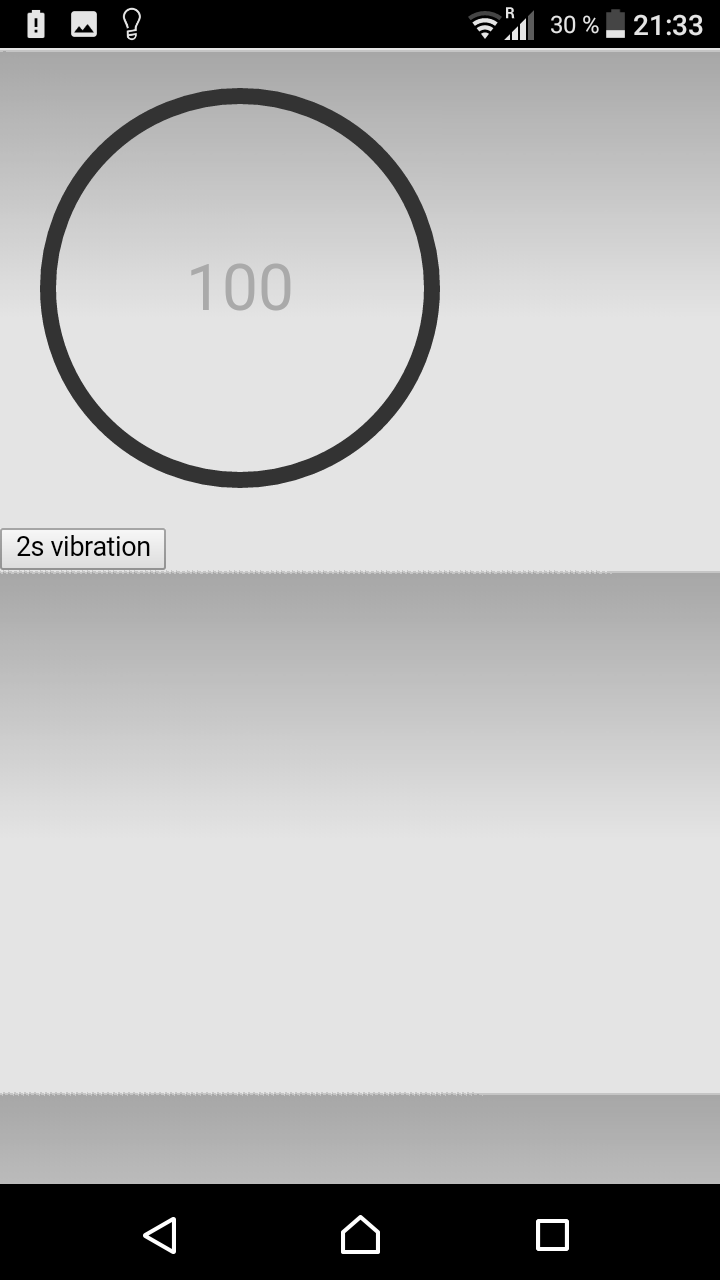
\includegraphics[width=0.22\textwidth]{Figures/cordova4android.PNG}
		& 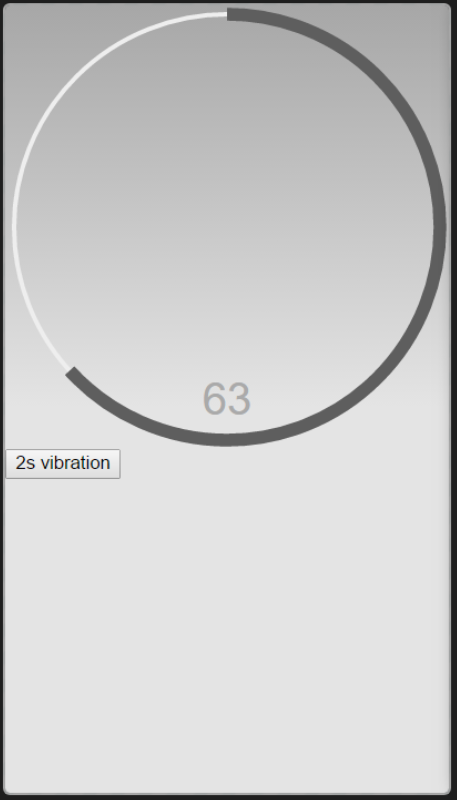
\includegraphics[width=0.22\textwidth]{Figures/cordova4ios.png}
		& 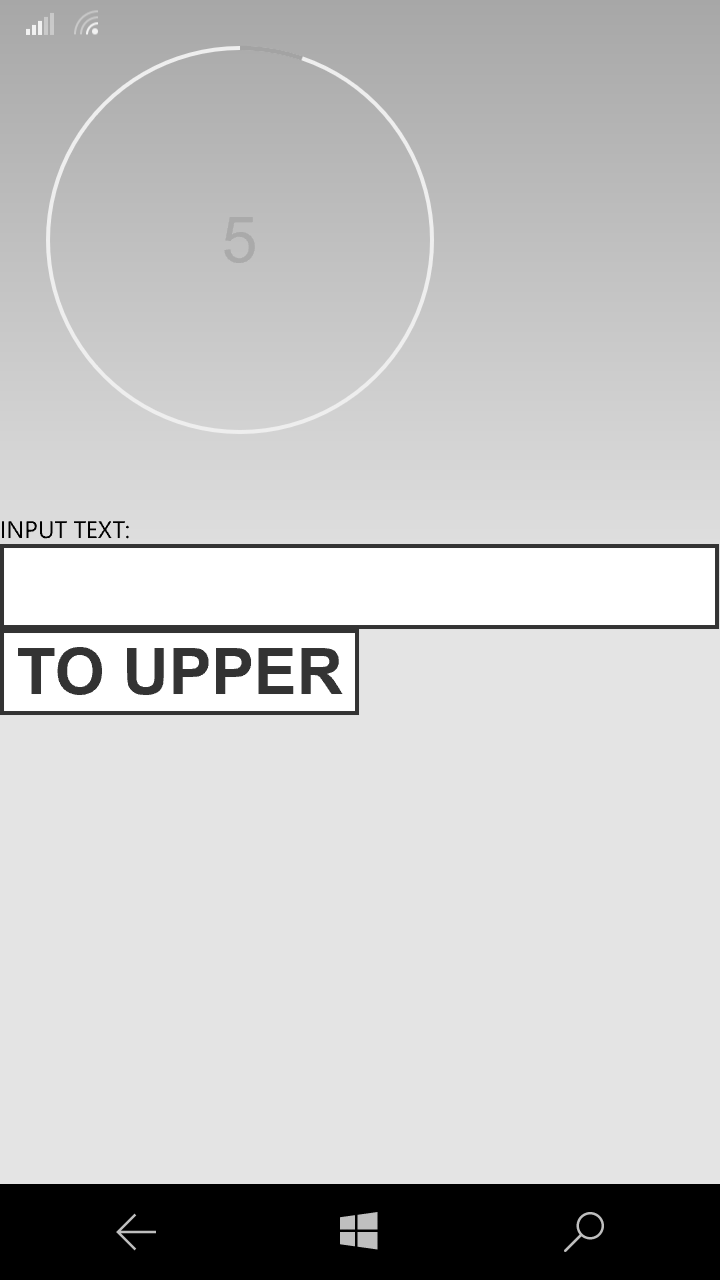
\includegraphics[width=0.22\textwidth]{Figures/cordova4windows.PNG}
		\\
		\midrule
		React Native	
		& 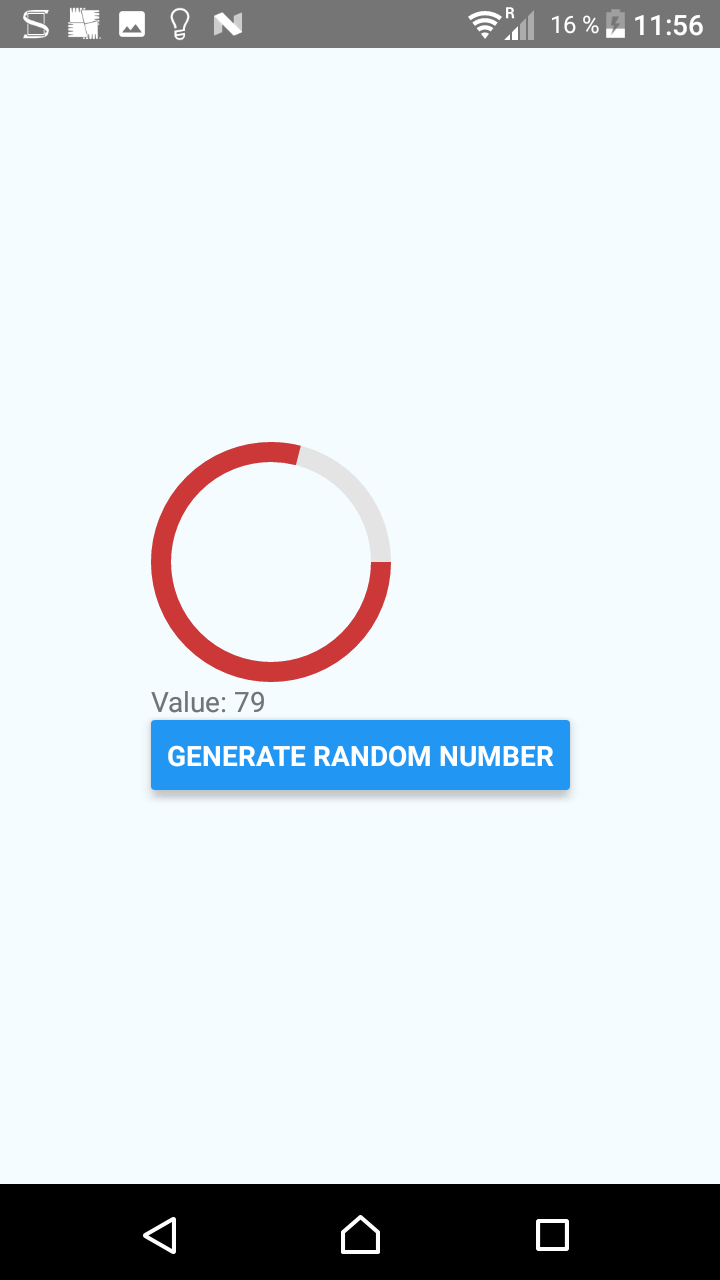
\includegraphics[width=0.22\textwidth]{Figures/react4android.PNG}
		& 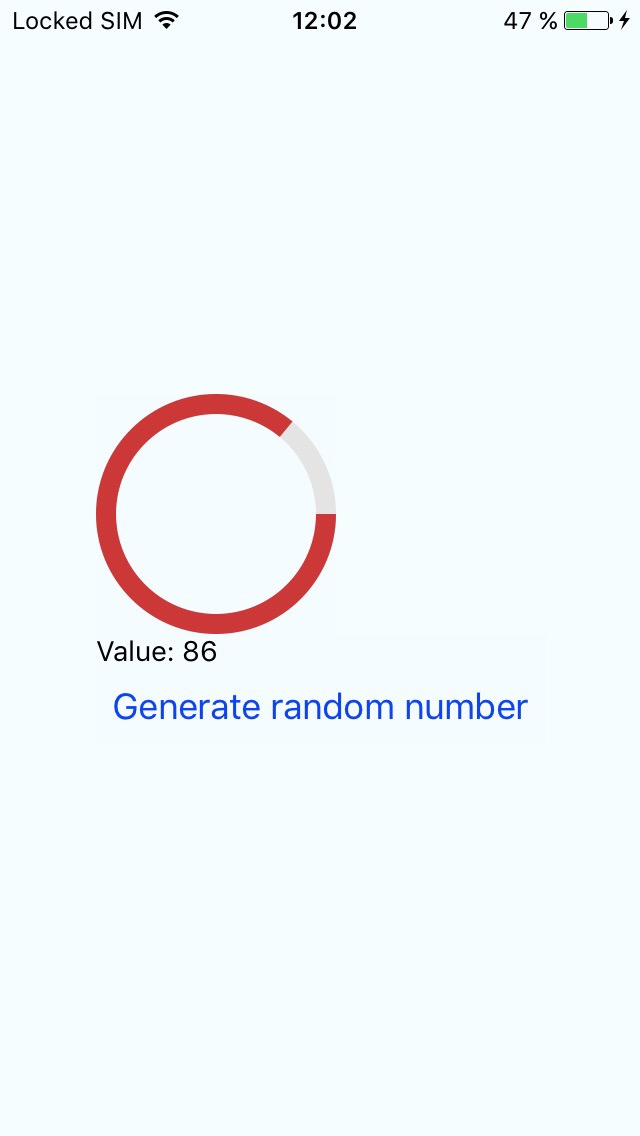
\includegraphics[width=0.22\textwidth]{Figures/react4ios.jpg}
		&
		\\
		\midrule
		Xamarin	
		& 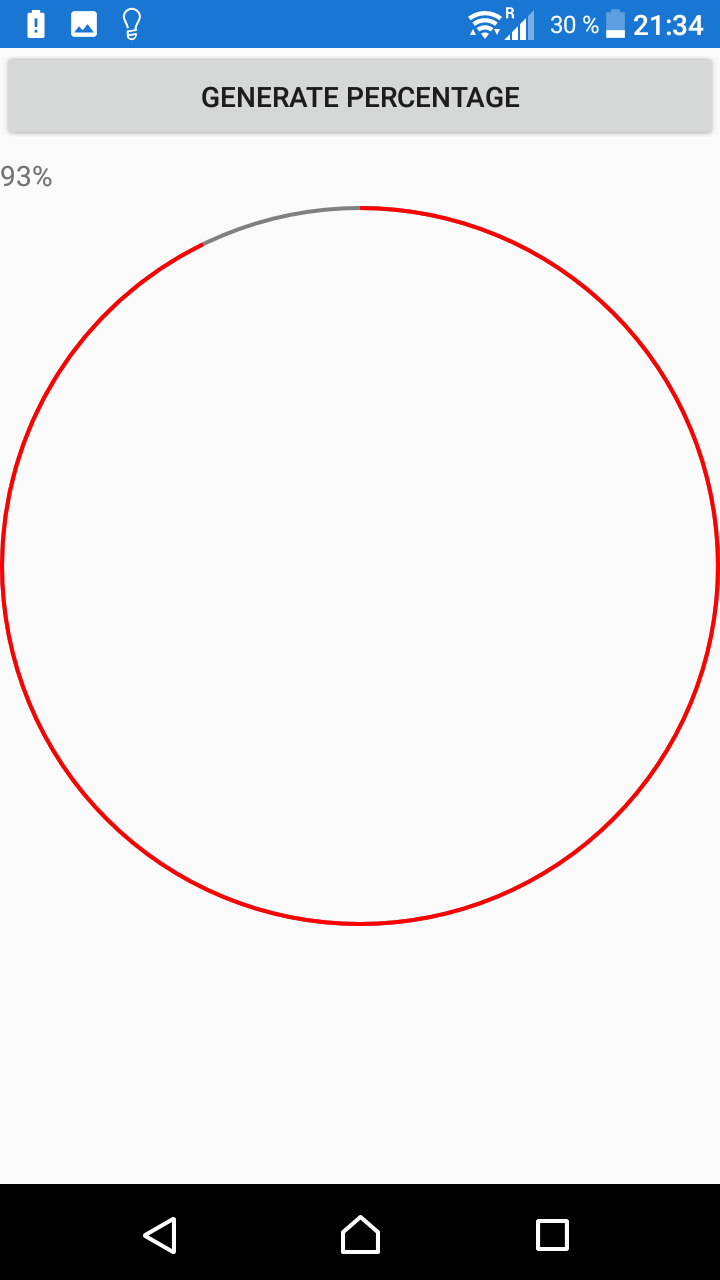
\includegraphics[width=0.22\textwidth]{Figures/xamarin4android.PNG}
		& 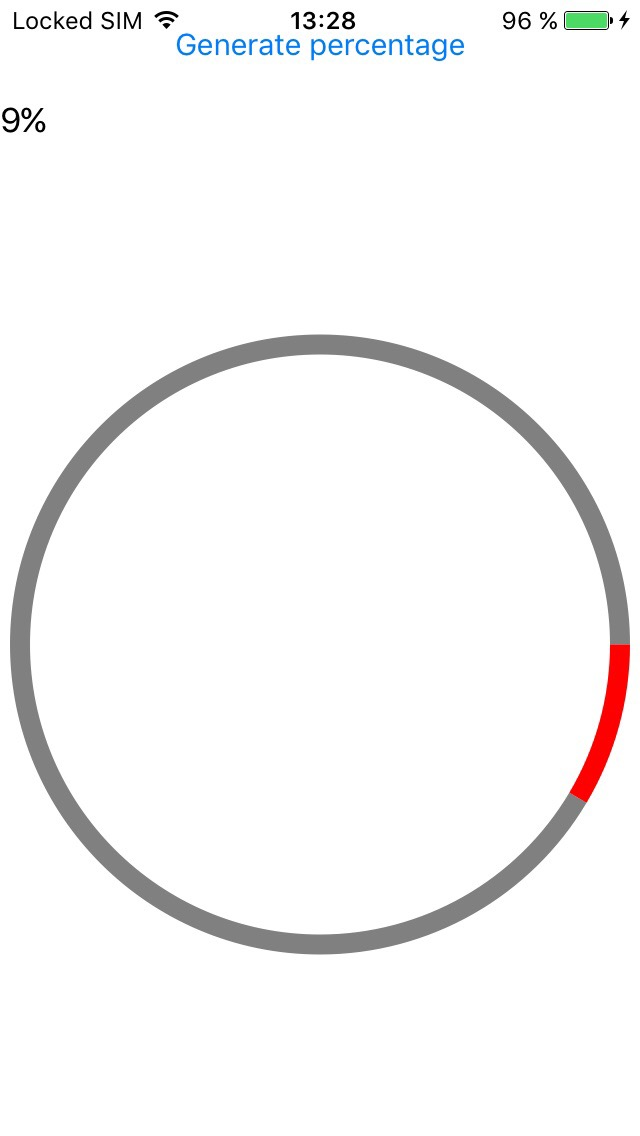
\includegraphics[width=0.22\textwidth]{Figures/xamarin4ios.jpg}
		& 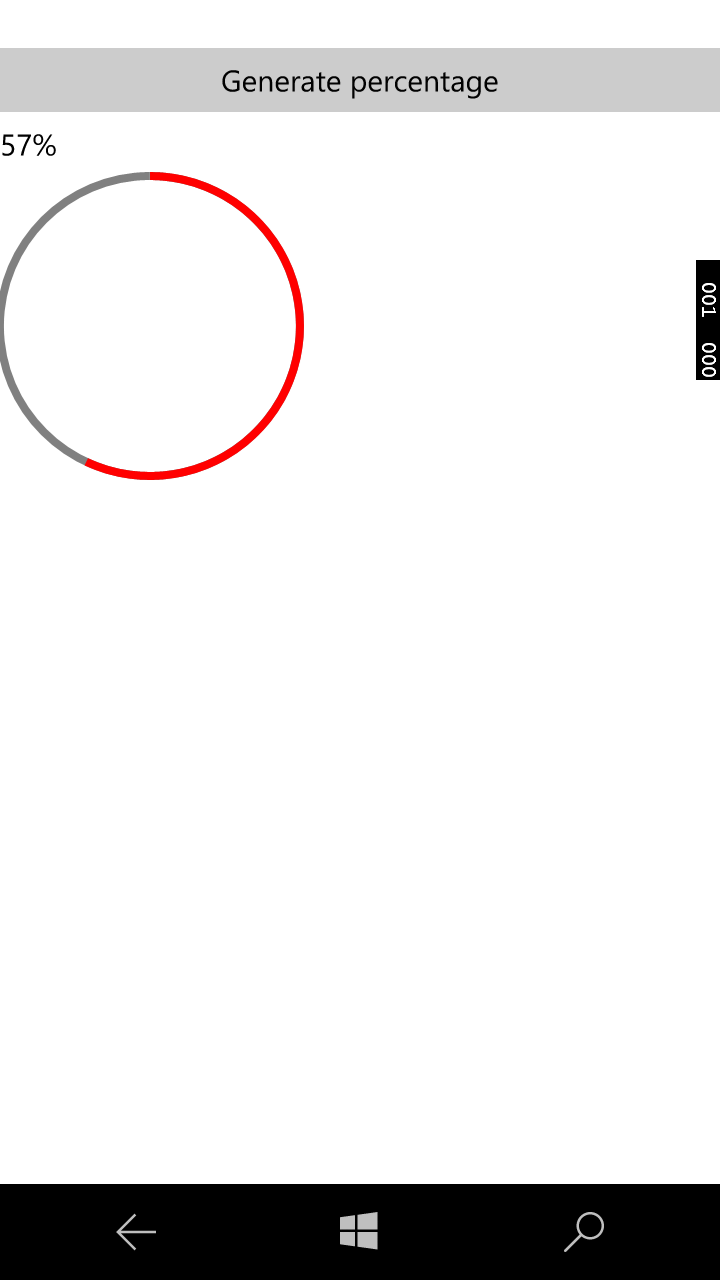
\includegraphics[width=0.22\textwidth]{Figures/xamarin4windows.PNG}
		\\
		\midrule
	\end{tabular}
\end{table}

\subsubsection{Setup}
Considering Apache Cordova, the initial setup for Android and Windows is rather easy since it is a plugin within Visual Studio. The built-in installation process automatically downloads and installs Node.js with Cordova CLI and Git CLI. It also prepares Apache Ant, Oracle Java JDK and Android SDK to enable Android development. Tools for Windows mobile development are not installed automatically. However, they can be added by ticking the checkboxes for Universal Windows Platform tools for Cordova and Windows 10 Mobile Emulator. 

Since iOS apps can be built only on a Mac, a separate setup is needed. Visual Studio provides the possibility to build the application remotely, so only few programs need to be installed - namely Node.js, Xcode and Xcode command-line tools. After enabling remote agent on Mac, Visual Studio can connect to it and build the iOS app remotely.

Regarding React Native, the attempt to run a Windows app with the React Native Windows plugin failed. With no reason to develop on a Windows machine, the development process was moved to a Mac. Similar to Apache Cordova, React Native required Node.js as well. In addition to the required React Native CLI, the installation of Watchman was recommended. For Android, Java Development Kit had to be installed. Next, a custom installation of Android Studio was performed, adding Android SDK, Android SDK Platform, Intel HAXM and Android Virtual Device. Since React Native does not support Android Nougat\footnote{As of early 2017}, Android Marshmallow SDK had to be downloaded as well (with several required sub-features). At last, the Android setup was finished by specifying the ANDROID\_HOME environment variable.

Compared to Android, iOS installation was incomparably easier. Besides the common tools for React Native development, only Xcode was required. In addition to that, WebStorm was installed as well, because of its superior IDE capabilities for JavaScript development.

Xamarin brings us back to Windows. Although Xamarin development is possible on Mac as well (with Xamarin Studio or Visual Studio for Mac), building a Windows app is possible only on Windows. Installing Xamarin is, again, easy via a Visual Studio plugin. By default, the plugin installs Xamarin, Android NDK, Android SDK, Java JDK, Google Android Emulator and Intel HAXM. In addition to that the user may choose to install Universal Windows Platform tools for Xamarin and Windows 10 Mobile Emulator. 

Again, installation on Mac has to be done separately. Visual Studio on Windows can reach out to a remote Mac, build there the iOS application and then display it back locally. Alternatively, Visual Studio can be installed on Mac, enabling development for Mac, iOS and Android. The code can be shared between Windows and Mac instances of Visual Studio via a remote repository.

\subsubsection{Hello World}
There were no issues with the first, very simplistic app. All tested frameworks passed the test almost flawlessly. The only problem was with jQuery for Windows in Apache Cordova project. For some reason, jQuery was added twice, thus the application did not work. Therefore, pure JavaScript was used for all Cordova apps.

\subsubsection{Persistent storage}
For persistent storage, SQLite database was chosen for Xamarin and Apache Cordova, while React Native app was integrated with Realm. 

Apache Cordova has multiple possibilities of storing data, such as file system storage or the web-browser-based Local storage and Indexed DB. However, only SQLite plugin provides true database features and is consistent across all tested platforms. The plugin worked properly when storing strings, floats and datetimes as well as automatically incrementing the primary key. However, since JavaScript cannot work with binary data, they had to be converted to base-64, even though the SQLite database was able to store it like a BLOB. Another issue on Windows was with toolset version 141, which had do be manually downgraded to 140. After that everything went smoothly.

Similarly to Cordova, also React Native had to work with base-64 binary objects. Moreover, the Realm implementation for React Native is not yet able to automatically generate IDs \footnote{as of early 2017}, thus random GUID was used the primary key. Although Realm provides greater abstraction over SQLite (which forces programmers to use pure SQL), it does have considerably less functionality. Yet, for small databases that is more than sufficient.

The last tested framework, Xamarin, implemented SQLite as well. The SQLite library for .NET provides the same amount of abstraction and Realm does for React Native, yet provides the full potential of SQL statements and functions just as pure SQLite for Apache Cordova. Its implementation is superior to both alternatives. Moreover, C\# has a larger variety of supported types, thus being able to manipulate with binary objects directly.

\begin{table}[!h]
	\centering
	\caption{React Native - Tablet layout optimization}
	\label{table:react6}
	\begin{tabular}{p{5cm} | p{5cm}  }
		\toprule		
		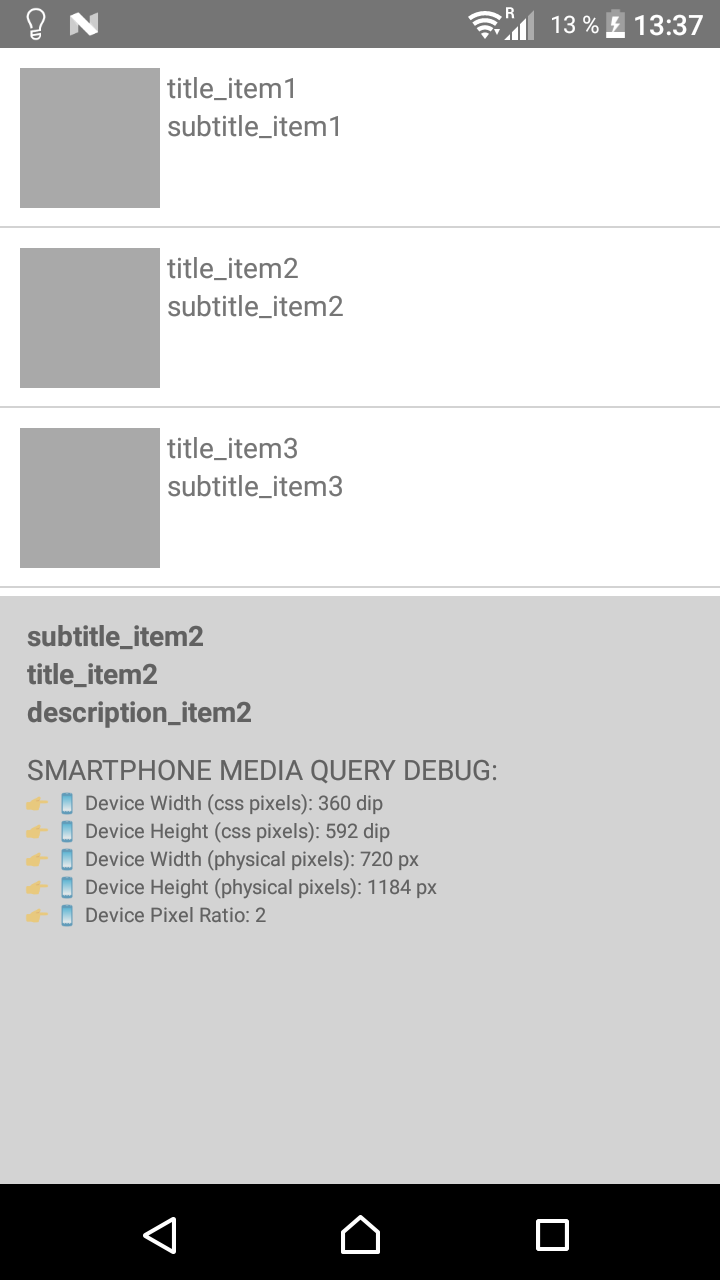
\includegraphics[width=0.3\textwidth]{Figures/react6android.PNG}
		& 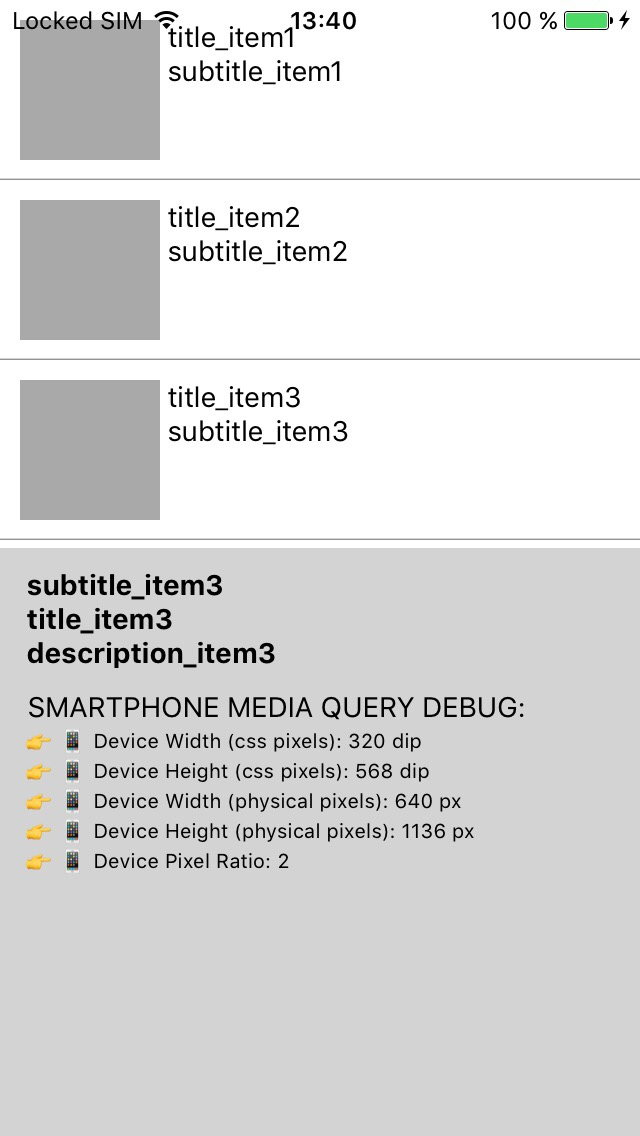
\includegraphics[width=0.3\textwidth]{Figures/react6ios.jpg}
		\\
		Android & iOS \\
		\midrule
	\end{tabular}
\end{table}

\subsubsection{Camera and location}
For a long time, Apache Cordova was the most popular multi-platform development tool, and it still belongs into top 3. It is therefore no surprise that it has a vast amount of 3rd party plugins and extensions, which help other developers achieve almost any desired functionality. For both camera and geolocation, Cordova offers official plugins, which worked flawlessly on all three platforms.

React Native offers geolocation functionality by default and it works perfectly both on Android and iOS. However, there is no official support for camera usage. Either a custom binding into native code (React bridge) has to be created, or a 3rd party library can be used. For our evaluation, custom library \cite{reactNativeCamera} was chosen, but unsuccessfully. The camera plugin did not work on neither of the tested platforms.

Xamarin for Android and Xamarin for iOS allow programmers to access the camera and geolocation just the way they would do it in a native Java or ObjectiveC application. However, Xamarin.Forms is an abstraction over platform-specific code and does not provide camera or geolocation functionality out of the box. Both of them can achieved either by custom implementation (injecting the platform-specific code into a common interface) or by using a 3rd party plugin. There are multiple GitHub repositories and NuGet packages offering extensibility to Xamarin.Forms, one of which was used also in this thesis \cite{xamarinPlugins}. On all three tested platforms both Media and Geolocator plugin worked without any issue. 

\subsubsection{Custom UI element and native code}
For all frameworks, a circular progress bar was chosen as a custom UI element. Since hybrid apps are just web apps wrapped in a native web view, creating a custom UI element is done via HTML, CSS and JavaScript, just like in any regular web page. Creating a custom circular progress bar in Apache Cordova took almost no time at all. 
The more challenging part was creating a bridge between the native code and JavaScript, since this required creating a whole new Apache Cordova plugin - a process requiring several steps for each platform. This was achieved only on Windows, by creating a simple functionality, which allowed converting lower case text into upper case. However, on Android and iOS only pre-built plugins worked. Therefore, Android and iOS apps call another plugin providing vibration capabilities.

Also in React Native the custom element was done almost immediately, since a 3rd party plugin exists. Unlike Apache Cordova, also the bridge between React code and native code was done rather easily. Since the build process of React Native includes a generated native infrastructure, it is possible to extend the infrastructure with custom code. A simple React annotation in ObjectiveC or Java than exposes the native classes and methods inside React Native.

The most complicated circular progress bar implementation was performed in Xamarin. Since the circular progress bar does not exist on any platform, it has to be implemented on each of them. Afterwards, a common element declaration is created in XAML in Xamarin.Forms. The last step is to tell Xamarin, how to render the common XAML declaration on individual frameworks - this is done via Custom Renderers. A Custom Renderer binds the common XAML element and its properties to the native element, its properties and rendering functionality.

Also, the bridge to native code can be done in two ways. The first one is very easy - dependency injection. Since C\# code in Xamarin is compiled to native code, platform specific classes inheriting from a common interface can contain native methods. In the common library, the interface is then used to instantiate the platform-specific code and invoke a particular method. The second approach can use real native JAR, AAR, DLL or Objective-C library. These are then inserted into the solution via a Binding Project, which enables direct method calls into the native library.

\subsubsection{PUSH notifications}
To avoid the tedious task of creating a new PUSH notification service for each platform-specific service provider (Apple Push Notifications Service, Google Firebase, Windows Notification Service), a multi-platform abstraction available via Microsoft Azure was leveraged. Its Notification Hub provides a single point of contact with the server code, so the web service does not have to contain individual calls to each notification service provider.

However, each service (APNS, Firebase, WNS) had to be configured via the Azure Portal. Google's Firebase is the only completely free provider. Both Windows as Apple require a paid developer certificate. While Windows developer certificate is relatively cheap and valid for a lifetime, the Apple developer certificate requires expensive annual payments. Due to this restriction, PUSH notifications on iOS were not tested \footnote{It is true that Google Firebase provides support also for iOS applications. However, this use-case is not covered in the Azure Notification Hub. Moreover, several authors claim that Firebase on iOS is highly unreliable, compared to APNS via Azure. Since tutorials for iOS PUSH notification services are available both for Apache Cordova and Xamarin, at least mock-up PUSH clients were implemented.}.

Considering the development in the mobile frameworks themselves, Microsoft Azure provides pre-build sample apps for Apache Cordova and Xamarin. Both of these apps were simple To-Do lists, which responded with a PUSH notification upon successfully adding a new To-Do item.

Since each mobile OS is connected to its own, platform-specific notifications service provider, parts of code had to be done platform-specifically. In case of Apache Cordova, this was handled by simply putting an if-else statement, checking the run-time platform. In case of Xamarin, the PUSH notification receivers had to be implemented for each platform specifically, thus resolving the client already during compilation. For Android, both a notification client and notification service receiver had to be implemented. The subscription to individual remote messages was based on a unique client ID, generated by Firebase. Windows had a much simpler implementation, with a single method opening an asynchronous channel to handle PUSH notifications. However, it required association with Microsoft Store via the developer certificate. The untested iOS implementation consisted of two methods - one for notifications subscription, the other for receiving remote notifications. The application would require an application-specific certificate, issued by APNS.

Following the usual convention, React Native comes with a plugin for Azure Notification Hub. Currently, it contains implementation only for Android and Windows. And since we were unable to run the Windows plugin, only Android implementation was tested. Just as for Apache Cordova and Xamarin, the React application had to be registered within Firebase to get a Sender ID. To be compatible with the existing server, parts of code from Apache Cordova had to be implemented. 

\subsubsection{Tablet optimization}
To demonstrate that the UI optimization for various screen sizes can be achieved by common techniques used in responsive web design, a simple demonstration web page from W3Schools was used \footnote{Can be found at: https://www.w3schools.com/w3css/tryit.asp?filename=tryw3css\_templates\_blog\&stacked=h} for Apache Cordova. The responsive app worked well on all three platforms, in both portrait and landscape modes. Plus, it displayed the expected behaviour on Windows 10 desktop.

The solution for responsiveness in React Native was, once again, a plugin. This plugin used the experimental EcmaScript 6 annotations. These annotations were then used as run-time conditions for React Native styles. Eventually, the whole process was not too dissimilar to media queries used in responsive CSS styles.

In platform-specific Xamarin implementations, responsiveness is handled on each platform individually. However, Xamarin.Forms provides an abstraction to this - device idiom. The value of Device.Idiom can be either Phone, Tablet or Desktop. This provides a run-time condition checking, similar to React Native. The app can then decide whether to render a XAML page optimized for phones, or for tablets.

\begin{table}[!h]
	\centering
	\caption{Xamarin - Tablet layout optimization on Windows devices}
	\label{table:xamarin6}
	\begin{tabular}{p{5cm} | p{11cm}  }
		\toprule		
		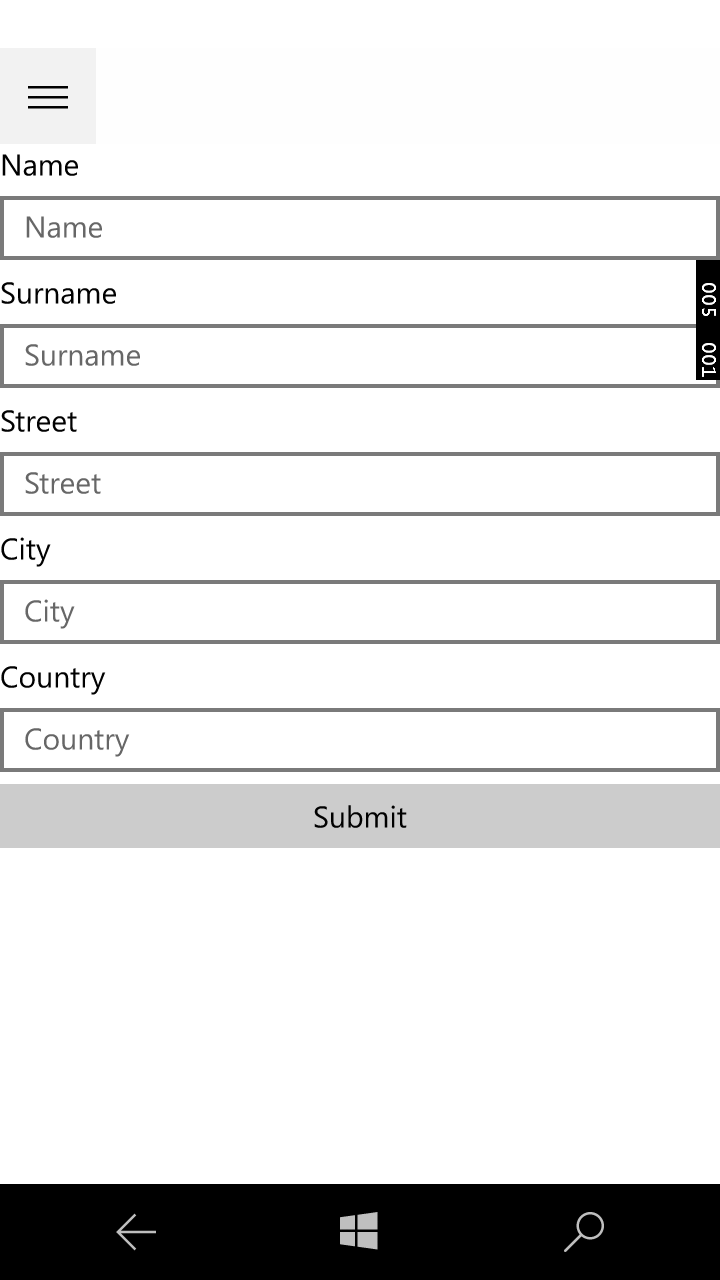
\includegraphics[width=0.3\textwidth]{Figures/xamarin6windows.PNG}
		& 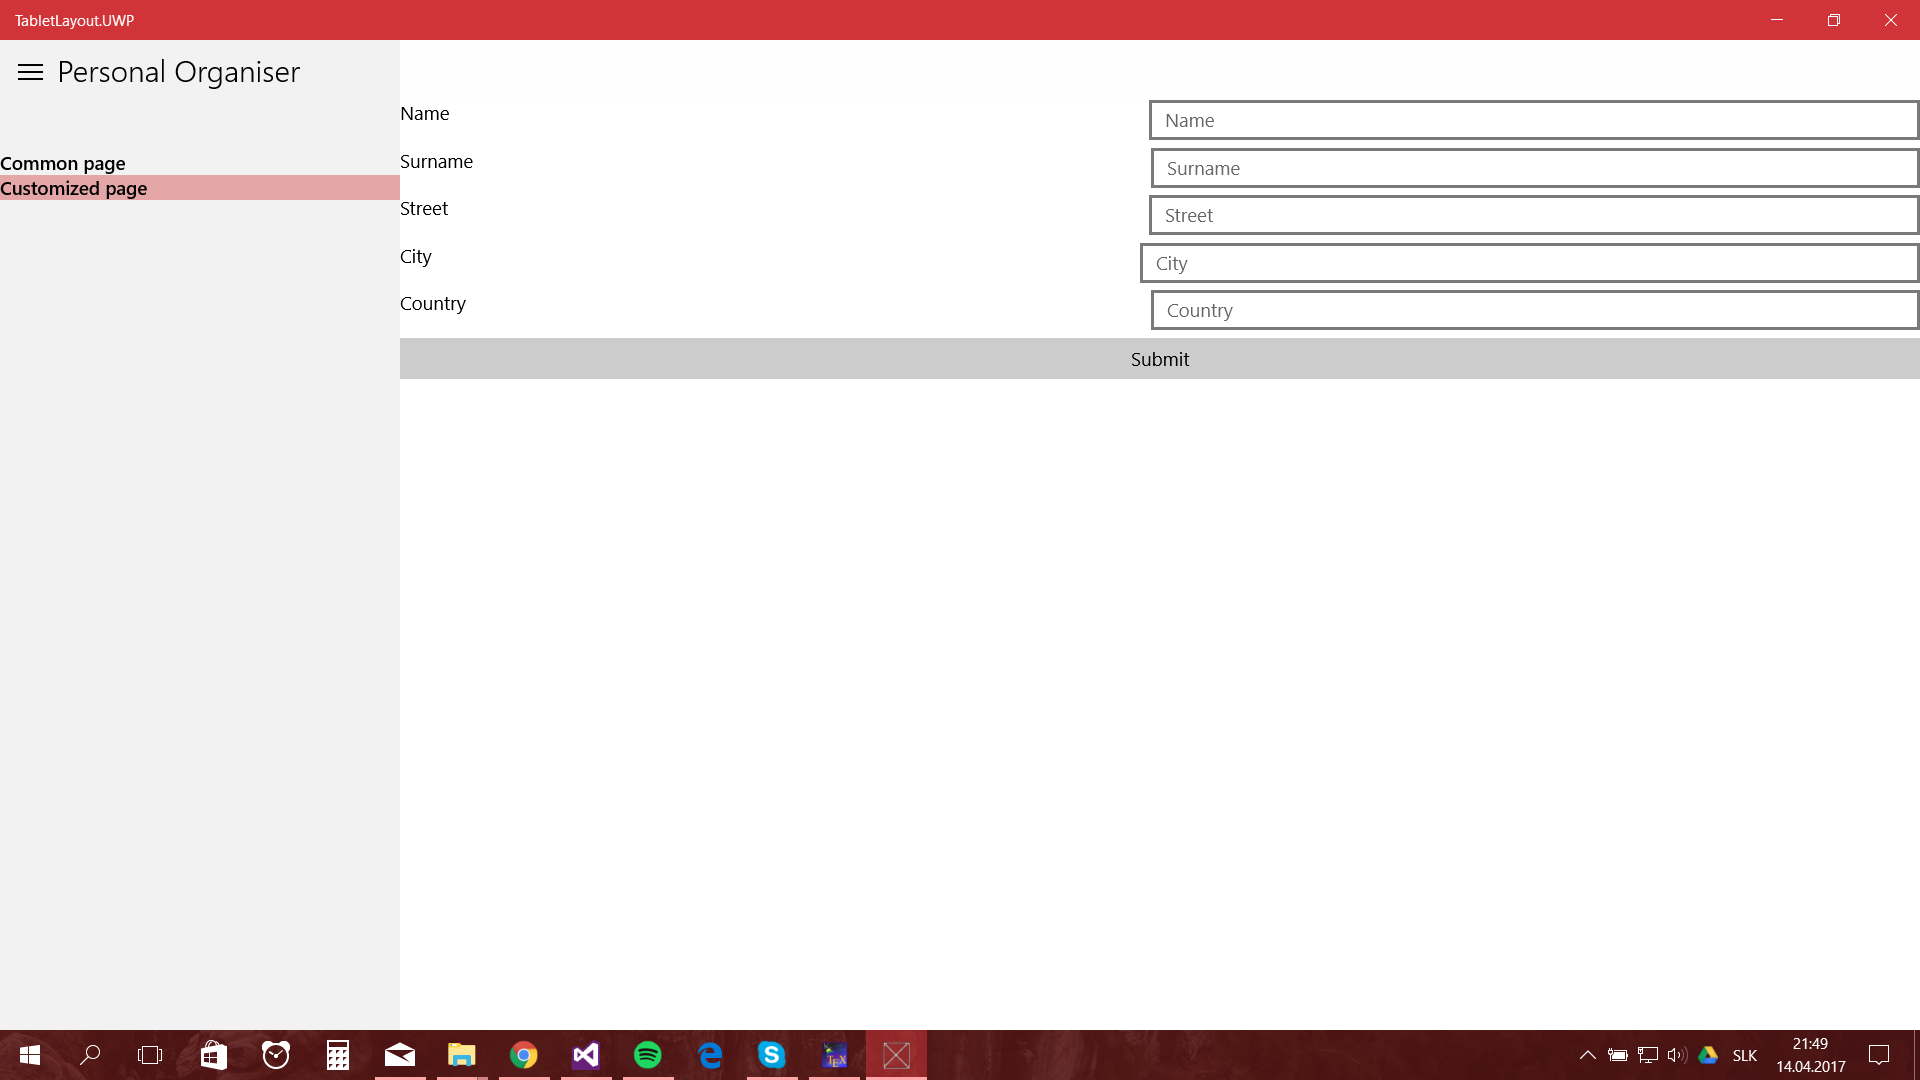
\includegraphics[width=0.7\textwidth]{Figures/xamarin6winx.PNG}
		\\
		Windows 10 Mobile & Windows 10 Desktop \\
		\midrule
	\end{tabular}
\end{table}

\subsubsection{Summary}
When summed together, it can be said that Apache Cordova is a very mature framework with great support and lots of 3rd party libraries, various guides and tutorials. It is very easy to learn and use it, especially for developers familiar with modern web technologies. Thanks to its rich set of plugins, almost any desired functionality is achievable. And the use of HTML, CSS and JavaScript the UI design and development is also straightforward. However, Apache Cordova is suitable only for small apps, which are not performance-demanding. Because the app runs in a browser, parts of native functionality is simply unavailable. The resulting applications are often bloated and rather slow. Last, but not least, the apps do not look native. This can be solved by using Ionic, which produces native-looking apps from Angular. However, it does not solve the other issues. 

Considering React Native, it takes a little time to learn the way, how it works and how to implement Redux, the most commonly used React architecture. Yet, the same principles apply also for web development in ReactJS, so developers can reuse this knowledge. After getting past this initial hurdles, the development in React Native is extremely fast. Npm is growing everyday with new React Native packages. However, React Native is still in development and many of its features are not yet production-ready, e.g.: Windows development, or camera usage. Its speed performance and the resulting app size are also not optimal. Yet, it can be expected that once React Native is finished, all this issues will be solved, or at least mitigated. For fast prototyping and small to medium-sized apps, React Native might be the right framework in the near future. Its closest competitor, NativeScript, uses Angular and provides slightly better performance, yet at the cost of smaller popularity (thus smaller community and less 3rd party libraries). It might be possible that React Native and other JavaScript interpreted frameworks will once render hybrid frameworks obsolete.

The last tested development tool, Xamarin, is the most difficult to learn, but is the most powerful at the same time. Unlike Apache Cordova or React Native, Xamarin provides only partial abstraction (in case of Xamarin.Forms) or almost no abstraction (in case of Xamarin.Android and Xamarin.iOS) over the native code. A lot of functionality that is quickly achievable in the other frameworks require more coding in Xamarin. Therefore, Xamarin is not suitable for prototyping and small projects. However, it provides the best control over native code, enables the usage of all native APIs and allows the usage of common design patterns and best practices. A vast amount of NuGet packages, 3rd party libraries and plugins can quickly enrich Xamarin with new functionality. Xamarin also produces apps with the smallest overhead and the best performance (there are benchmarks in which Xamarin surpassed even native Java on Android). Due to these factors, Xamarin is best suited for medium to large-scale applications, or applications with demanding and complicated functionality.



\section{Methodology}

There exist multiple texts comparing a couple of multi-platform development tools \cite{aarhus} \cite{uppsala} \cite{taxonomyCP}. Some of them even provide guide or explanation on how the tools were chosen and how to pick the most suitable one for particular projects \cite{rhoMobile} \cite{aComparativeStudy}. However, there is no comprehensive methodology, generic enough to cover a wide variety of multi-platform frameworks. From the theoretical and practical information we have gathered in previous chapters, it is possible to construct a series of methodological steps that will achieve exactly this goal.

\subsection{Necessary preconditions}
If the methodology is supposed to be effective in the process of selecting the right tool, several preconditions need to be satisfied. The most important factor is specification. Of course, it is impossible to determine every single part of the resulting application right from the start. However, the more precise the specification, the more accurate results can be expected. 

The architect, business analyst or product owner should be aware also of the long-term vision for the next iterations. It is very unlikely that a prototype will be done in one tool, which will have to be switched for another, because of changed requirements. Most customers have neither enough money nor time.

Another important factor is to collect as much data about the available resources as possible. Enough information about the size, expertise and maturity of the development team can reduce both time and costs dramatically. Also, mapping already available software and hardware can help to keep the budget.

\begin{figure}
	\centering\fbox{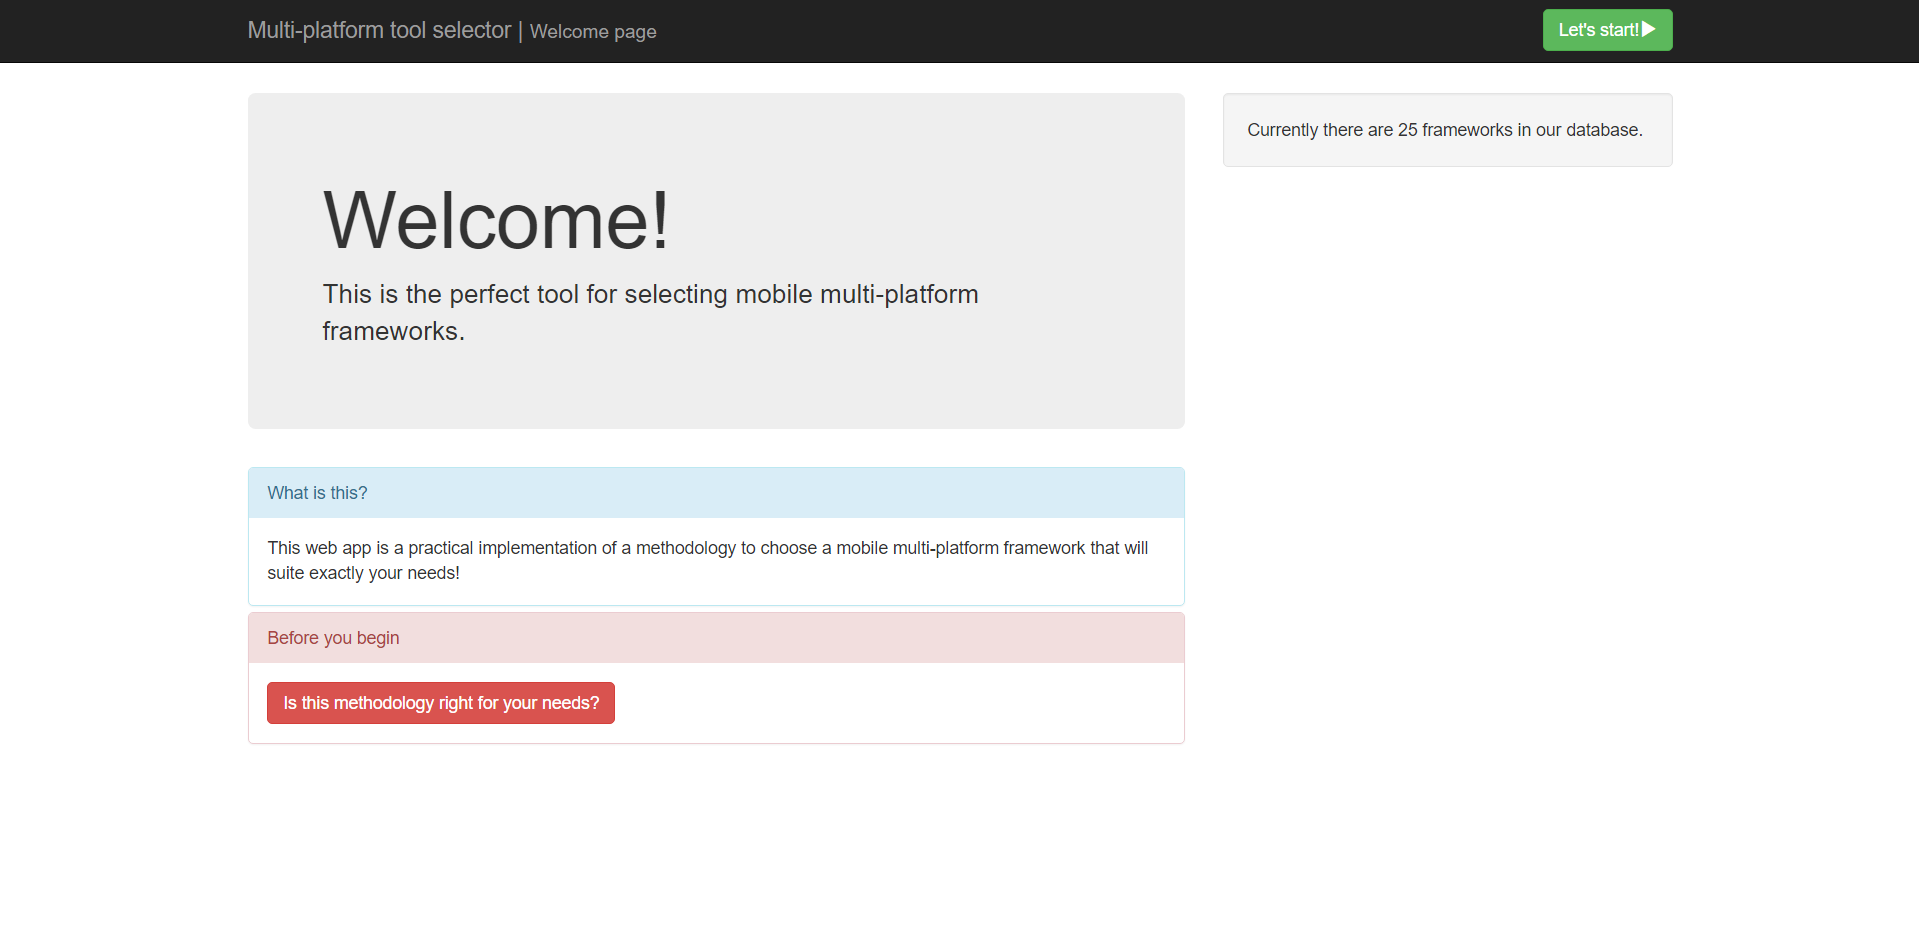
\includegraphics[width=0.8\textwidth]{Figures/welcome.png}}
	\caption{Welcome page of the methodology web app}
	\label{figure:webWelcome}
\end{figure}

\subsection{Methodologically unsuitable projects}

Before proceeding with the methodology itself, several eliminating questions should be answered. If the answer is “yes” to one or multiple questions, given project cannot be correctly assessed by this methodology.

\begin{itemize}
	\item \textbf{Is only one operating system (even with multiple screen sizes) targeted?} 
	If the answer is “yes”, then there is no reason to use multi-platform framework. There is nothing that beats native development. The world of multi-platform tools is a world of compromises. Native development allows to use the operating system to its fullest potential, while not limiting the performance. If Java or ObjectiveC are concerns, there exist alternatives also for single-platform development, such as Swift or Kotlin.
	
	\item \textbf{Do you want to target operating systems other than Android, BlackBerry, iOS and Windows?} 
	This methodology is aimed strictly on mobile OSs. Although some tools allow development for desktop computers as well, this possibility is not discussed in the methodology. From those featured in the methodology, Qt, Embarcadero, Kivy, RubyMotion or Xamarin target also one or multiple desktop platforms. 
	
	The key operating systems for this methodology are Android and iOS. Attention is paid also to Windows support (namely Windows 10 UWP and Windows 8.1 WinRT). Tools enabling development for BlackBerry are examined for their full support. However, should the reader want to focus on different mobile operating systems (like Symbian, Bada or others), this methodology and the suggested results may not be suitable for that use case.
	
	\item \textbf{Will the app use extensively multiple platform-specific APIs, sensors or widgets?} 
	Many platform-specific features (like Android widgets or Windows life tiles) are not present on other operating systems, thus several multi-platform development tools ignore them altogether. Since the focus of multi-platform tools is to run a single common code on multiple platforms, they often use the road of least common denominator and strip away features, which have no alternatives on other platforms. Some tools provide platform overrides, or allow to have platform-specific application and UI layers. Yet, if the design and functionality for each OS is significantly different\footnote{An example of this may be something as simple as a slider. While on iOS and Windows the native slider allows arbitrary steps, the Android SeekBar is bound to 1000 steps. As a result, values not divisible by 1000 broke the application, since the slider could not find the right position. It took several days to determine the cause of the issue and write a reliable platform-agnostic solution}, a multi-platform tool is useless. 
	
	Tools with active community may have various 3rd party resources, but these may complicate the licencing, increase the cost, decrease performance and violate the security. Adding a large quantity of libraries or plugins will increase the size of the application dramatically. 
	
	\item \textbf{Do you want to create a game?} 
	Although some multi-platform development tools studied by this methodology allow game development to certain extent, for a fully-fledged 2D or 3D game it may not be appropriate. Discussing the differences between individual game framework is beyond the scope of this work. Multi-platform frameworks allowing game development include (but are not limited to) Unity 3D, Unreal Development Kit, Marmelade, MoSync or Wave. However, should the reader plan creating multiple apps and wish to utilize the invested learning effort, he/she is advised to use the methodology and focus on tools supporting game development.
	
	\item \textbf{Do you want to create a new web app for both desktop and mobile, or port an existing desktop web page to mobile environment?} 
	If the project is a web page or web application that should be available both for mobile and desktop environment and there is no intention of using native APIs or sensors, mobile web app frameworks should be considered. They produce a common web page, adjusted for the mobile devices. For starters, Bootstrap Mobile, AppPress, Sencha Touch, Dojo or jQuery Mobile should be examined. 
	
	\item \textbf{Do you want to create a business-focused enterprise application with connection to an existing cloud backend?}
	This thesis focuses on frameworks, which allow general-purpose app creation. However, there is a plethora of tools and services which can create a single-purpose app (e.g. for monitoring of employees, to provide ERP and CRM services). Examples of such tools can be Appticles, i-exceed, Pega Systems or Retriever Communications. 
	
	Other group of single-purpose multi-platform tools focus on providing MBaaS services. They integrate into existing cloud systems (like AWS, Azure, Oracle, IBM, SAP or Salesforce) and enable data access and management from a mobile app. Providers of these services include nypresence, AppGyver, IBM Mobile First, Kinvey, MobileFrame, MooFWD. There is plenty of others, not covered in this thesis. However, MBaaS providers who allow creating offline apps and multi-purpose apps have been added to the main methodology.
\end{itemize}


\begin{figure}
	\centering\fbox{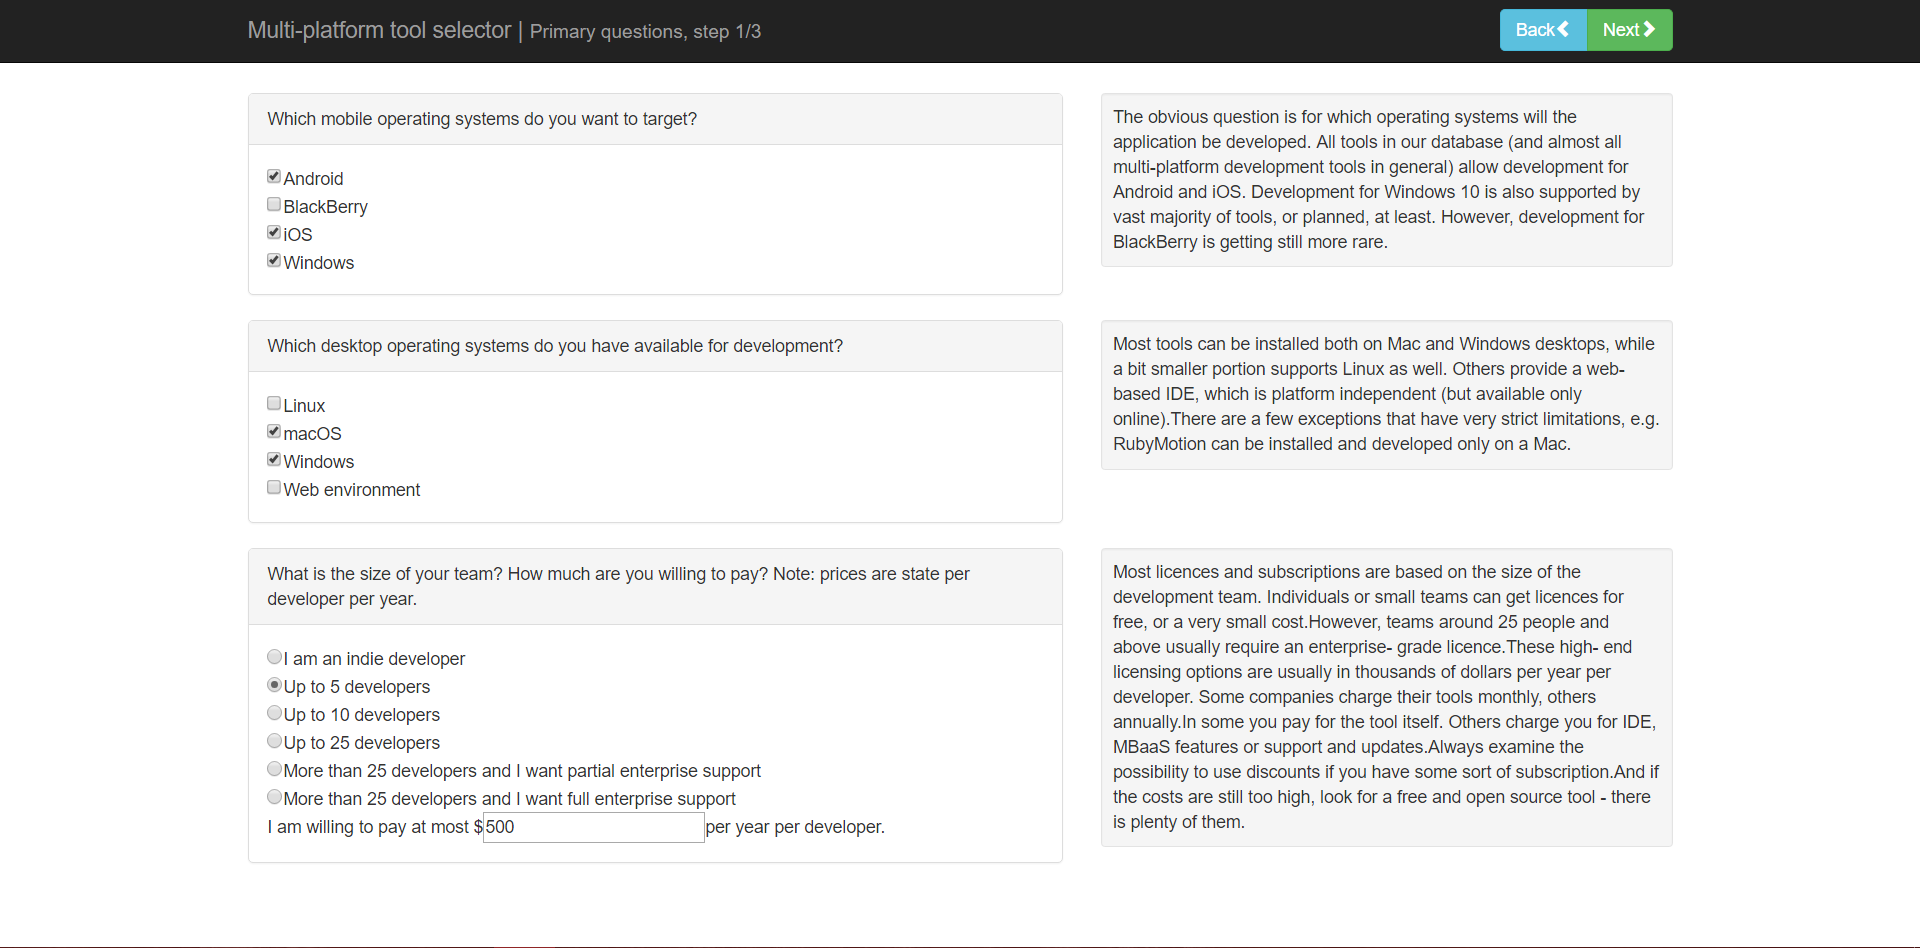
\includegraphics[width=0.8\textwidth]{Figures/questions.png}}
	\caption{Questions page of the methodology web app}
	\label{figure:webQuestions}
\end{figure}

\subsection{Recommended way of using the methodology}
If the project has passed all questions from chapter 5.2, it means it is suitable to be subjected to the methodology. The whole methodology consists of 4 sets of questions. Each set has decreasing importance. The first set of questions is the most important. Tools not fulfilling requirements posed in this set violate the project's specification radically. Such tools should be removed from further evaluation.

\begin{figure}
	\centering\includegraphics[width=0.45\textwidth]{Figures/Methodology.png}
	\caption{Recommended way of using the methodology}
	\label{figure:activityMethodology}
\end{figure}
	
It is possible that for certain projects the most suitable multi-platform development tool will be clear already after the first set of questions. However, usually the first set of question selects a small group of frameworks with similar capabilities. To distinguish which of them is the most appropriate for a certain project, the second set of questions should be taken. This set contains conditions which are fairly common in mobile app development. Failing one or two requirements in the second set is not as critical as in the first set. Usually, there exists a work-around, but it may increase the project cost, development time or negatively impact app's performance.
	
Projects having unusual or highly specific requirements should be subjected also to the third set of questions. This set contains conditions which are rare, or there exists an easy workaround. It also focuses on features that may help to decrease the development time or increase performance, user experience and stability of an application. Either way, after the second or third set of questions, the majority of project will get a clear recommendation on which framework to use.
	
If there is no clear winner even after the third set of questions, then there is the last set of questions. These supplementary questions have no clear answer. They rather point out further criteria which can be researched to discover the most suitable development tool.
	
If not explicitly said otherwise, each question in the first three sets can be answered in three different ways: yes, nice to have and no. Yes means the feature or condition mentioned in the question is necessary in the application and cannot be skipped. Nice to have describes a feature, which is not crucial for the application or has not been included in the requirements, but could improve the performance or UX of the project. No means the condition is irrelevant to the project.
	
Similarly, each feature or condition can be fulfilled by the framework in one of three ways: yes, partially and no. Yes means the feature is fully supported by the development tool. Partially means the feature can be implemented, but it comes with a hiccup. The option "partially" usually comes with a note further describing the limitation. No means the feature is completely absent in the framework. Combination of possible answers and requirement implementations results in an evaluation matrix, as seen in table \ref{table:evaluationMatrix}.
	
\begin{table}[!h]
	\centering
	\caption{Evaluation matrix}
	\label{table:evaluationMatrix}
	\begin{tabular}{p{3cm} | p{3cm} | p{3cm} | p{3cm}}
		\toprule
		\textbf{The user wants it: / The framework has it:} & \textbf{Yes} & \textbf{Partially} & \textbf{No} \\
		\midrule
		\textbf{Yes} & +7 / +5 / +3 points & 0 / 0 / 0 points & Excluded from evaluation / -5 / -3 points \\
		\midrule
		\textbf{Nice to have} & +7 / +5 / +3 points & 0 / 0 / 0 points & -7 / 0 / 0 points \\
		\midrule
		\textbf{No} & 0 / 0 / 0 points & 0 / 0 / 0 points &  0 / 0 / 0 points \\
		\midrule	
	\end{tabular}
\end{table}

Particular way of assigning points is described at the beginning of each set of questions. Questions, which have a different way of assigning points, describe the process in place. A short example of assigning points can be found in the following subchapter.

\subsubsection{Example score evaluation}
For the purpose of brevity, we will compare only four tools - Codename One, Ionic, NeoMAD and ViziApps. Also the specification will be very simple. The application should run on Android, iOS and Windows. There should be a separate layout for tablets and phones. The app will work via WiFi, but occasional Bluetooth capability is a nice-to-have feature.

First, we will prepare a table. The columns will be filled with the names of the development tools. The rows will be used for adding points.

\begin{table}[!h]
	\centering
	\caption{Sample evaluation - step 1}
	\label{table:sampleEvaluation1}
	\begin{tabular}{p{2.5cm} | p{2.5cm} | p{2.5cm} | p{2.5cm} | p{2.5cm}}
		\toprule
		& \textbf{Codename One} & \textbf{Ionic} & \textbf{NeoMAD} & \textbf{ViziApps} \\
		\midrule
		\textbf{Total} &&&& \\
		\midrule
	\end{tabular}
\end{table}
	
Then we continue through the methodology and examine all necessary questions. We will write the answers in the form of points each tool scored.

\begin{table}[!h]
	\centering
	\caption{Sample evaluation - step 2}
	\label{table:sampleEvaluation2}
	\begin{tabular}{p{2.5cm} | p{2.5cm} | p{2.5cm} | p{2.5cm} | p{2.5cm}}
		\toprule
		& \textbf{Codename One} & \textbf{Ionic} & \textbf{NeoMAD} & \textbf{ViziApps} \\
		\midrule
		\textbf{Can create Android app?} & +7 & +7 & +7 & +7 \\
		\textbf{Can create BlackBerry app?} & 0 & 0 & 0 & 0 \\
		\textbf{Can create iOS app?} & +7 & +7 & +7 & +7 \\
		\textbf{Can create Windows app?} & +7 & +7 & +7 & Excluded \\
		\midrule
		\textbf{Total} &&&& \\
		\midrule
	\end{tabular}
\end{table}

The first requirement for our sample project is to target Android, iOS and Windows. Since this question belongs to the first set, we operate with the step of 7 points. Let us apply the evaluation matrix from table 13. BlackBerry is not relevant to our project, so we choose the "No" row. As we can see, all frameworks gain 0 points for BlackBerry implementation - regardless of whether they support it or not. However, for Android, iOS and Windows we apply the "Yes" row. All frameworks, which support a platform gain +7 points per platform. There is no framework that would partially support a platform, so none gets 0 points for Android, iOS or Windows. However, ViziApps does not support development for Windows platform. Failing any "Yes" question in the first set results in immediate exclusion of a development tool from further evaluation. Thus we continue only with 3 frameworks in the next step.

\begin{table}[!h]
	\centering
	\caption{Sample evaluation - step 3}
	\label{table:sampleEvaluation3}
	\begin{tabular}{p{2.5cm} | p{2.5cm} | p{2.5cm} | p{2.5cm} | p{2.5cm}}
		\toprule
		& \textbf{Codename One} & \textbf{Ionic} & \textbf{NeoMAD} & \textbf{ViziApps} \\
		\midrule
		\textbf{Can create Android app?} & +7 & +7 & +7 & +7 \\
		\textbf{Can create BlackBerry app?} & 0 & 0 & 0 & 0 \\
		\textbf{Can create iOS app?} & +7 & +7 & +7 & +7 \\
		\textbf{Can create Windows app?} & +7 & +7 & +7 & Excluded \\
		\midrule
		\textbf{Is it possible to adjust the layout for phone and tablet?} & -5 & +5 & +5 & - \\
		\midrule
		\textbf{Total} &&&& \\
		\midrule
	\end{tabular}
\end{table}

UI responsiveness to various screen sizes is a question from the second set. Once again, we look at the "Yes" row of the evaluation matrix. Questions from the second set are evaluated by 5 points. Immediately, we can see that Codename One does not support various screen layouts. For the second set of questions, the punishment for failing a condition are not that harsh. We do not remove Codename One from further evaluation, but we subtract 5 points from its score. Ionic and NeoMAD, on the other hand, both provide functional layout adjustments, so they both gain 5 points. We proceed to the last, voluntary feature.

\begin{table}[!h]
	\centering
	\caption{Sample evaluation - step 4}
	\label{table:sampleEvaluation4}
	\begin{tabular}{p{2.5cm} | p{2.5cm} | p{2.5cm} | p{2.5cm} | p{2.5cm}}
		\toprule
		& \textbf{Codename One} & \textbf{Ionic} & \textbf{NeoMAD} & \textbf{ViziApps} \\
		\midrule
		\textbf{Can create Android app?} & +7 & +7 & +7 & +7 \\
		\textbf{Can create BlackBerry app?} & 0 & 0 & 0 & 0 \\
		\textbf{Can create iOS app?} & +7 & +7 & +7 & +7 \\
		\textbf{Can create Windows app?} & +7 & +7 & +7 & Excluded \\
		\midrule
		\textbf{Is it possible to adjust the layout for phone and tablet?} & -5 & +5 & +5 & - \\
		\midrule
		\textbf{Is Bluetooth supported?} & 0 & +3 & 0 & - \\
		\midrule
		\textbf{Total} &&&& \\
		\midrule
	\end{tabular}
\end{table}

Implementing Bluetooth is not a necessary condition, thus we use the "Nice to have" row from the evaluation matrix. Bluetooth capability belongs to the third set of questions, rated with 3 points. Neither Codename One, nor NeoMAD provide an out-of-the box support for Bluetooth. A 3rd party library, or custom implementation has to be used instead. Thus, they gain 0 points. Ionic, which comes with Bluetooth support directly, gains 3 points. When all questions have been answered, we can continue to the final evaluation

\begin{table}[!h]
	\centering
	\caption{Sample evaluation - step 5}
	\label{table:sampleEvaluation5}
	\begin{tabular}{p{2.5cm} | p{2.5cm} | p{2.5cm} | p{2.5cm} | p{2.5cm}}
		\toprule
		& \textbf{Codename One} & \textbf{Ionic} & \textbf{NeoMAD} & \textbf{ViziApps} \\
		\midrule
		\textbf{Can create Android app?} & +7 & +7 & +7 & +7 \\
		\textbf{Can create BlackBerry app?} & 0 & 0 & 0 & 0 \\
		\textbf{Can create iOS app?} & +7 & +7 & +7 & +7 \\
		\textbf{Can create Windows app?} & +7 & +7 & +7 & Excluded \\
		\midrule
		\textbf{Is it possible to adjust the layout for phone and tablet?} & -5 & +5 & +5 & - \\
		\midrule
		\textbf{Is Bluetooth supported?} & 0 & +3 & 0 & - \\
		\midrule
		\textbf{Total} & 19 & 29 & 26 & - \\
		\midrule
	\end{tabular}
\end{table}

After counting all the points, we can see that Ionic is the most suitable framework for our particular project, with NeoMAD being close in second place. Codename One is far behind and ViziApps did not even make it through the first round. However, for other projects the results can be totally different. If the reader was not still decided whether to use Ionic or NeoMAD, he/she can research further facts, such as how good is the documentation, how buggy is the tool or what other apps have been created using the particular framework.

\subsection{Primary questions}

\begin{figure}
	\centering\includegraphics[width=0.8\textwidth]{Figures/ActivityDiagram7.png}
	\caption{Evaluation process for primary questions}
	\label{figure:activityPrimary}
\end{figure}

This is the first and most important set of questions. Majority of the questions are crucial to all applications. Questions that are irrelevant to your project should be skipped. All tools that do not satisfy at least one condition in this first category should be removed. There might be some tools that have partial or planned support for some of the conditions. It depends on your particular use case whether this limitation can be accepted or not. 

\begin{enumerate}
	\item \textbf{Does the tool support all required mobile operating systems? (Evaluation matrix, 7 points for each required and supported platform)}
	The obvious question is for which operating systems will the application be developed. All tools mentioned in this thesis (and almost all multi-platform development tools in general) allow development for Android and iOS. Development for Windows 10 is also supported by vast majority of tools, or planned, at least. However, development for BlackBerry is more difficult, since only 4 tools out of the 23 featured in this thesis fully support development for this OS.
	
	\item \textbf{Does the tool support development on desktop operating systems you own? (Evaluation matrix, 7 points for each required and supported platform)}
	Most tools can be installed both on Mac and Windows desktops, while a bit smaller portion supports Linux as well. Others provide a web-based IDE, which is platform independent (but available only online). There are a few exceptions that have very strict limitations, e.g. RubyMotion can be installed and developed only on a Mac. 
	
	\begin{enumerate}
		\item \textbf{Does the tool allow iOS builds on Windows/Linux? (Evaluation matrix, 7 points) }
		If you own at least one Mac or do not wish to target iOS, you can skip this question. While Android applications can be built on any desktop OS, projects for iPhones and iPads require compilation on a Mac device. Some tools (like Aquro, Codename One, Smartface and ViziApps) remove this obstacle by providing cloud-based builds. You do not need to buy a Mac, but you must accept that your project is being compiled somewhere in the cloud.
		
		\item \textbf{Does the tool allow Windows builds on Mac/Linux? (Evaluation matrix, 7 points) }
		If you own at least one Windows PC or do not wish to target Windows mobile platform, you can skip this question. Similar to iOS, also Windows mobile requires builds on a Windows desktop machine. Unlike macOS, however, you can install Windows on a virtual machine, side by side with your Linux or Mac, so this problem is solved easier. Yet, you still need at least one Windows license. If you want to avoid buying a Windows PC, or software license, Appery.io, Codename One, Tabris and Telerik Platform offer cloud builds for Windows mobile.
	\end{enumerate}
	
	\item \textbf{How much are you willing to pay? What licensing do you need? What is the size of your team? (compare with the offered prices, do not assign any points, but remove tools which fail your requirements) }
	Most licences and subscriptions are based on the size of the development team. Individuals or small teams can get licences for free, or a very small cost. However, teams around 25 people and above usually require an enterprise-grade licence. These high-end licensing options are usually in thousands of dollars per year per developer. 
	
	Some companies charge their tools monthly, others annually. In some you pay for the tool itself. Others charge you for IDE, MBaaS features or support and updates. Always examine the possibility to use discounts if you have some sort of subscription. And if the costs are still too high, look for a free and open source tool - there is plenty of them.
	
	\item \textbf{Do you want the UI to look the same on all operating systems, or use the native look and feel? Does the tool support it? (do not assign any points, but remove tools which fail your requirements) }
	Even with a single shared UI code, the application may still look native on individual platforms. Many tools offer the possibility of transforming the platform-agnostic UI code into platform-specific UI elements. Others take a different approach and give the possibility for the app to look exactly the same on Android, iOS and Windows. Both approaches have their pros and cons and it depends on each project what is most suitable for them. Kivy, Kony, Qt and most of the hybrid frameworks give the opportunity to have the same look and feel across all operating systems. Appcelerator, Embarcadero, Ionic and Xamarin are examples of tools that take the native UX approach.
	
	\begin{enumerate}
		\item \textbf{If you chose native look, do you want to code a single UI layer for all operating systems, or a custom layer for each mobile OS? Does the tool support it? (do not assign any points, but remove tools which fail your requirements) }
		While some projects need to do rapid prototyping, others may want to facilitate the opportunities brought by each platform. If your project needs to implement different UI for each OS (e.g. to use the Android fragments, which are not available on iOS), you might want to look at tools like Appcelerator, NativeScript, React Native, RubyMotion or Xamarin. However, all of the platforms studied by this thesis provide also the possibility to write a single UI layer for all target platforms. This allows almost 100\% code sharing, but reduces the available UI elements to the lowest common denominator.
	\end{enumerate}
	
	\item \textbf{Does your project require multithreading and does the development tool support it? (Evaluation matrix, 7 points) }
	Downloading, uploading, calling remote web services, image and sound processing or other computation-heavy calculations are all examples of tasks, which take some time. During this time the app should still be responsive and, perhaps, be able to schedule also further tasks. This requires using multiple threads - one serving the UI responsiveness and the others doing the tasks in background. If the project contains a large portion of functionality involving multitasking, you should avoid all JavaScript-based tools (both hybrid and interpreted). JavaScript does not support threading on a language level, and while there are workarounds using web workers, their implementation is inferior, compared to traditional threads. Using C++, C\#, Java, Python or Ruby should handle the situation just fine.
	
	\item \textbf{Do you want to access the media, use the camera and microphone, play audio and video? Does the tool provide the API? (Evaluation matrix, 7 points for each required and supported feature) }
	Capturing photos and videos is one of the most common hardware interfaces used in mobile applications. While all studied development tools allow taking photos, not all of them are able to capture video or record sounds (Kivy, Kony, NativeScript, React Native). For example, there exists a 3rd party library for Kivy, but it allows recording sounds only for Android. Even the consecutive replay of recorded sound or video is not warranted in all tools - it is completely absent in Instant Developer, and a 3rd party library is needed for NativeScript and React Native.
	
	\item \textbf{Do you want to use geolocation, accelerometer or gyroscope? Does the tool provide the API? (Evaluation matrix, 7 points for each required and supported feature) }
	The global and relative positioning of the mobile device is another functionality often used in an application. Accessing GPS and navigation is offered out-of-the-box in all tools, except of Kivy and Smartface. However, using accelerometer or gyroscope needs a 3rd party library or custom implementation in Kivy, NativeScript, React Native and Smartface.
	
	\item \textbf{Do you want to access the device state (battery status, network availability, OS version, etc.)? Does the tool provide necessary APIs? (Evaluation matrix, 7 points) }
	Although this functionality is not usually required, particular applications may change their behaviour due to low battery power or unstable Internet connection. Yet, some tools do not provide this information (Corona, Kony, ViziApps) or rely on 3rd party libraries or custom implementation (Codename One, Kivy, Qt, React Native).
	
	\item \textbf{Do you want to use a background process? Does the tool support them? (Evaluation matrix, 7 points) }
	Some applications might find it useful to have a permanent background service with no interface. This could be applied for several use cases, like tracking the position, updating stock markets data, notifying user of an emergency situation. You should take into consideration, that iOS has very limited support for background processes, allowing only geolocation updates. All other background functionality is restricted (with the exception for VoIP applications). The only possible workaround is using remote push notifications. Android, BlackBerry and Windows allow creating background processes, but their implementation and requirements may differ. In all cases, you should keep in mind that background processes on any platform are considered low priority. Therefore they are the first victims when the underlying OS needs to kill running apps and get more resources.
	
	Because of these obstacles, only a handful of tools provide a way to create background services (Codename One, Embarcadero, NeoMAD, Qt, Xamarin). Although there exist 3rd party libraries for all tools based on Apache Cordova, their functionality is limited and inconsistent across individual operating systems.
	
	\item \textbf{Do you want to use PUSH notifications? Does the tool support them? (Evaluation matrix, 7 points) }
	Unlike local notifications, which are both sent and received by the application itself, push notifications are one of the few ways how a remote server can alert your application without prior request. They are important on Android and Windows, since there are still limited ways for push-model communication. However, they are absolutely essential on iOS, because it is the only way to replace background processes. It should be noted, that notifications differ a lot on individual platform. On Android, they are the most customizable, allowing various sorts of interaction, customization and binding functionality. It is possible to create interactive notifications on Windows as well. However, iOS are very limited, offer almost no interactivity and - in case the application is in background - push notifications are handled by the operating system itself, rather than the hosting application. 
	
	Push notifications are well established in tools providing MBaaS services, as it is one of their core functionalities. Yet, they are such an essential feature nowadays, almost all multi-platform development tools implement them (with Kivy and Qt supporting only Android and Windows notifications).
	
	\item \textbf{Do you need to create custom plugins or invoke native libraries? Does the tool support it? (Evaluation matrix, 7 points) }
	Even with the richest environment of 3rd party plugins, there can still be a custom library or UI element that is only available as a native C\#/Java/ObjectiveC/Swift package. You may also want to target a specific device, which has non-standard API, such as ambient lights. To do so, you need to interact with the native package either through a wrapper, or directly. Most tools provide one way or another to achieve this capability. But code-free tools, like Instant Developer, SmartFace or ViziApps have limited to no support for such behaviour.
	
	\item \textbf{Is app monitoring and crash analytics required by the project? Are they supported by the tool? (Evaluation matrix, 7 points) }
	Even when the app is out, the work is not done. Monitoring usage, performance and application crashes is vital for providing continual support and improvement. While there are some free libraries and tools like ACRA, Crashlytics or Xcode Crash Reports, they may not be compatible with your chosen development tool. You should closely examine, whether integration of the multi-platform development tool and analytics framework is possible. If not, try to find out, whether an alternative is provided by the tool (e.g. Telerik Analytics for NativeScript or HockeyApp for Xamarin).
\end{enumerate}

\subsection{Secondary questions}

\begin{figure}
	\centering\includegraphics[width=0.8\textwidth]{Figures/ActivityDiagram5.png}
	\caption{Evaluation process for secondary questions}
	\label{figure:activitySecondary}
\end{figure}

This set of questions contains conditions that are important for some applications, while irrelevant to others. Failing a condition in this category may seriously affect the development process, but a sort of workaround is usually possible.

\begin{enumerate}
	\item \textbf{How would you characterize the complexity of your app? (Add +5 if the framework has desired performance. Add 0, if the performance is higher. Subtract -5 if the performance is lower.)}
	Complexity of the application can help to determine which tool and programming language to choose. Simple, straight-forward applications can take advantage of the rapid prototyping provided by hybrid mobile applications and tools using scripting languages. Larger and more complex projects should be programmed in a strongly-typed programming language featuring object-oriented programming and separation of code into modules.
	
	\item \textbf{Is designer or previewer tool available? (Evaluation matrix, 5 points) }
	A design or preview tool allows to see the changes in UI code immediately on a simulated mobile device screen. Some allow also WYSIWYG editing. This can highly improve the communication between a designer, product owner and the developer. It can be also very helpful in rapid prototyping and agile development.
	
	\item \textbf{Do you want to have different UI for phone and tablet? Does the tool support multiple or responsive layouts? (Evaluation matrix, 5 points) }
	There are apps that look good on all screen sizes. And then there are apps that need radical layout changes to ensure good user experience both on smartphones and tablets. Most tools offer the possibility to create different layout for smaller and larger screens, or use the CSS responsive design in case of web technologies. Corona, for example, uses conditional compilation to render the right layout on a device. However, there is a number of tools (Aquro, Codename One, Instant Developer, Kivy, Qt, Tabris, ViziApps) that have no support for different UI layouts. The only way, to create a tablet-specific design is to create a separate application.
	
	\item \textbf{Does the design include any platform-specific overrides? Does the tool support them? (Evaluation matrix, 5 points) }
	Even if most parts of the application will be the same on all operating systems, there might be one or two things that will differ in order to maintain the native UX. While almost all tools achieve this either by replacing code files, conditional compilation or dependency injection, there are a few exceptions which do not support platform-specific overrides, namely Instant Developer, Smartface and ViziApps.
	
	\item \textbf{Will the application work with the file system? Is the tool able to access and manage it? (Evaluation matrix, 5 points) }
	All studied development tools provide access to the file system, although there might be some restrictions for Qt and hybrid apps. It is worth mentioning, that the file system structure differs a lot on Android, iOS and Windows. 
	
	\item \textbf{Will the application require persistent storage? Can the tool work with app properties or mobile database? (Evaluation matrix, 5 points for each required and supported database) }
	Excluding file system, Android, iOS and Windows offer 2 different approaches to data persistence. Simple key-value data pairs, such as the current application state or settings are usually saved in the app properties (SharedPreferences/NSUserDefaults/ApplicationDataContainer). More complex data structures are usually stored in a database. The most common database used in mobile world is SQLite, which has almost universal support across the studied tools. Couchbase and Realm are examples of other popular mobile database engines, also supported by several tools. Aquro and ViziApps are the only two multi-platform development tools not allowing any client-side data storage, since they rely on all data being stored in the cloud.
	
	\item \textbf{Do you want to use Bluetooth, NFC, fingerprint or barcode scanner? Is their API available in given tool? (Evaluation matrix, 5 points for each required and supported feature) }
	Unlike the other sensors, Bluetooth, NFC and fingerprint scanners are not software-related, but depend on the hardware outfit. This makes their availability fragmented even within an operating system. Only a small portion of studied tools provide the functionality out-of-the box. The majority relies on 3rd party libraries, or custom wrappers invoking native functionality. This is true also for the barcode or QR scanner - although it is captured by camera, it is processed usually by the native API.
	
	\item \textbf{Is integration with assistant service (Alexa, Cortana, Google Assistant, Siri) possible? (Evaluation matrix, 5 points for each required and supported assistant)} 
	Although the usage of AI-powered virtual assistance is still limited to several use cases and language, their possibilities are growing with each new update. Already now, virtual assistants are able to pick the best suited application for a particular request. If you want your application to be popular, it should communicate with the virtual assistant. Not all tools provide necessary support for this behaviour.
	
	\item \textbf{Does the tool support debugging? (Evaluation matrix, 5 points) }
	Debugging is one of the earliest tools that can help developers find and fix possible errors. It allows to closely examine every line of code. For any application that has medium to high complexity, debugging capability is a must.
	
	\item \textbf{Does the tool support unit testing? (Evaluation matrix, 5 points) }
	Unit tests are the first tests done after (or sometimes before) a piece of code is written. While not examining the system as a whole, they test each method or class individually. This helps to increase the clarity and readability of code. Unit tests are then the first indicator whether new or refactored code is functional and satisfies all required standards.
	
	\item \textbf{Does the tool support automated UI testing? (Evaluation matrix, 5 points) }
	While new functionality is generally thoroughly tested manually, repeated tasks, such as smoke tests or regression tests, can be automated. Automated UI tests substantially increase the volume of tests performed for complex business- and enterprise-ready applications. They can be also incorporated into the continuous integration process.
	
	\item \textbf{Does the tool support app profiling? (Evaluation matrix, 5 points) }
	Neither unit tests, nor manual tests are able to discover low-level or long-running issues, like memory leaks or taking up too much resources. If high quality and high performance are important for your project, you should definitely use a tool or IDE that provides app profiling.
\end{enumerate}



\subsection{Tertiary questions}

\begin{figure}
	\centering\includegraphics[width=0.8\textwidth]{Figures/ActivityDiagram3.png}
	\caption{Evaluation process for tertiary questions}
	\label{figure:activityTertiary}
\end{figure}

Following questions have either low impact on the application development or relate to a very small niche of projects and a workaround is possible. Yet, they still may balance the scales in one way or another. They serve as a finishing touch after the coarse separation in first two categories.

\begin{enumerate}
	\item \textbf{Does the tool allow development in a programming language you already have experience with? (Evaluation matrix, 3 points for each required and supported language) }
	Even if the developers have no previous experience with a multi-platform development tool, high skills in a particular programming language might help them to learn using it more quickly. 
	
	Currently, the most wide-spread programming language for multi-platform development is JavaScript, or some of its derivatives (Angular, TypeScript). However, there exists at least one or two tools for each major programming language (BASIC, C++, C\#, Delphi, Java, Lua, Python, Ruby). There are even a few tools which allow code-free visual app building.
	
	\item \textbf{Are MBaaS features or cloud connection necessary? Are they available? (Evaluation matrix, 3 points) }
	Many project rely on at least some basic cloud connectivity. Interaction with backend server or social networks is exactly what MBaaS providers offer. If the development tool does not feature an out-of-the-box MBaaS support, check the possibility of custom implementation. Especially code-free and JavaScript-based tools are prone to inability to add custom functionality.
	
	\item \textbf{Do you need an embedded web browser? Does the tool allow its use? (Evaluation matrix, 3 points) }
	Using an embedded web browser is one of the less common functionalities. Its use is very peculiar in case of the hybrid apps, since they themselves are ran from within a web browser - therefore, it is a browser inside a browser. Yet, with the exception of Instant Developer and Smartface, all tools support this functionality. Ionic, Kivy and NeoMAD require custom implementation and PhoneGap does not feature web browser for BlackBerry.
	
	\item \textbf{Do you want to access the address book and be able to make a call, or send SMS? Does the tool provide all necessary APIs? (Evaluation matrix, 3 points) }
	While contemporary smartphones are often more smart than phones, accessing the contacts list, making calls or texting is still used, from time to time. It is therefore a bit of relief that all examined development tools support this functionality, although some may require a 3rd party library.
	
	\item \textbf{Is a testing environment for multiple devices required? Does the tool feature any? (Evaluation matrix, 3 points) }
	Even automated tests on an emulator or real device have one major shortfall - they test only a single screen size. Screen fragmentation is a long lasting and well known issue on Android devices, but with the support for older hardware it is relevant also in the iOS and Windows world. Amazon Web Services provide a service known as Device Farm \cite{awsDeviceFarm}, which allows simultaneous UI testing on hundreds of physical Android and iOS devices in the cloud. Similar services are offered also by BitBar \cite{bitbar}, Firebase \cite{firebase} and TestObject \cite{testObject}. Some of the multi-platform development tools featured in this thesis provide also a cloud testing service, arguably with better integration with their product line (e.g. Telerik and Xamarin). If your app has the potential of being installed by millions of users, testing it on a Device Farm, or similar service, may be highly beneficial.
	
	\item \textbf{Does the tool allow continuous integration, if necessary? (Evaluation matrix, 3 points) }
	Continuous integration is a crucial part of DevOps, enabling small but valuable and rapid updates of an product or service. The whole process consists of various steps, like from coding, collaboration, versioning, unit and automatic testing to packaging, releasing and configuration management. A tool that can be easily incorporated into the process can result in shorter development cycles and higher customer satisfaction.
	
	\item \textbf{Are closed test groups required and supported? (Evaluation matrix, 3 points) }
	While all major application stores feature the possibility to share a WIP app to a tester group (Apple TestFlight, Google Play Testing, Windows Package Flights), some multi-platform development tools offer incorporated features of app distribution, giving you even more control. ViziApps, for example, offers the possibility of OTA (Over the Air) updates of installed apps.
	
	\item \textbf{Is OpenGL or WebGL required? Is it supported? (Evaluation matrix, 3 points) }
	There are some applications that may find use in hardware-accelerated 3D graphics. A model catalogue, design studio or a game are some examples of this kind of apps. Rendering and managing a 3D object requires the use of OpenGL library specialized for mobile or web environment. Most tools support the integration of either OpenGL ES or WebGL. However, Aquro, Instant Developer, Smartface and ViziApps are exceptions to this rule.
	
	\item \textbf{Does the tool support creating 2D games, if necessary? (Evaluation matrix, 3 points) }
	Although for a full-featured game development a mobile game framework would be more suitable, some multi-platform development tools are mature enough to host a simple 2D game. Examples of them can be Corona Labs, Kivy, Qt or Xamarin.
	
	\item \textbf{Does the tool support augmented or virtual reality, if necessary? (Evaluation matrix, 3 points) }
	Although augmented and virtual reality applications are dominated by games, various utility and even business apps are getting still more popular as well. Implementing one of these technologies might be exactly the thing that will set your app apart from the competition.
\end{enumerate}

\begin{figure}
	\centering\fbox{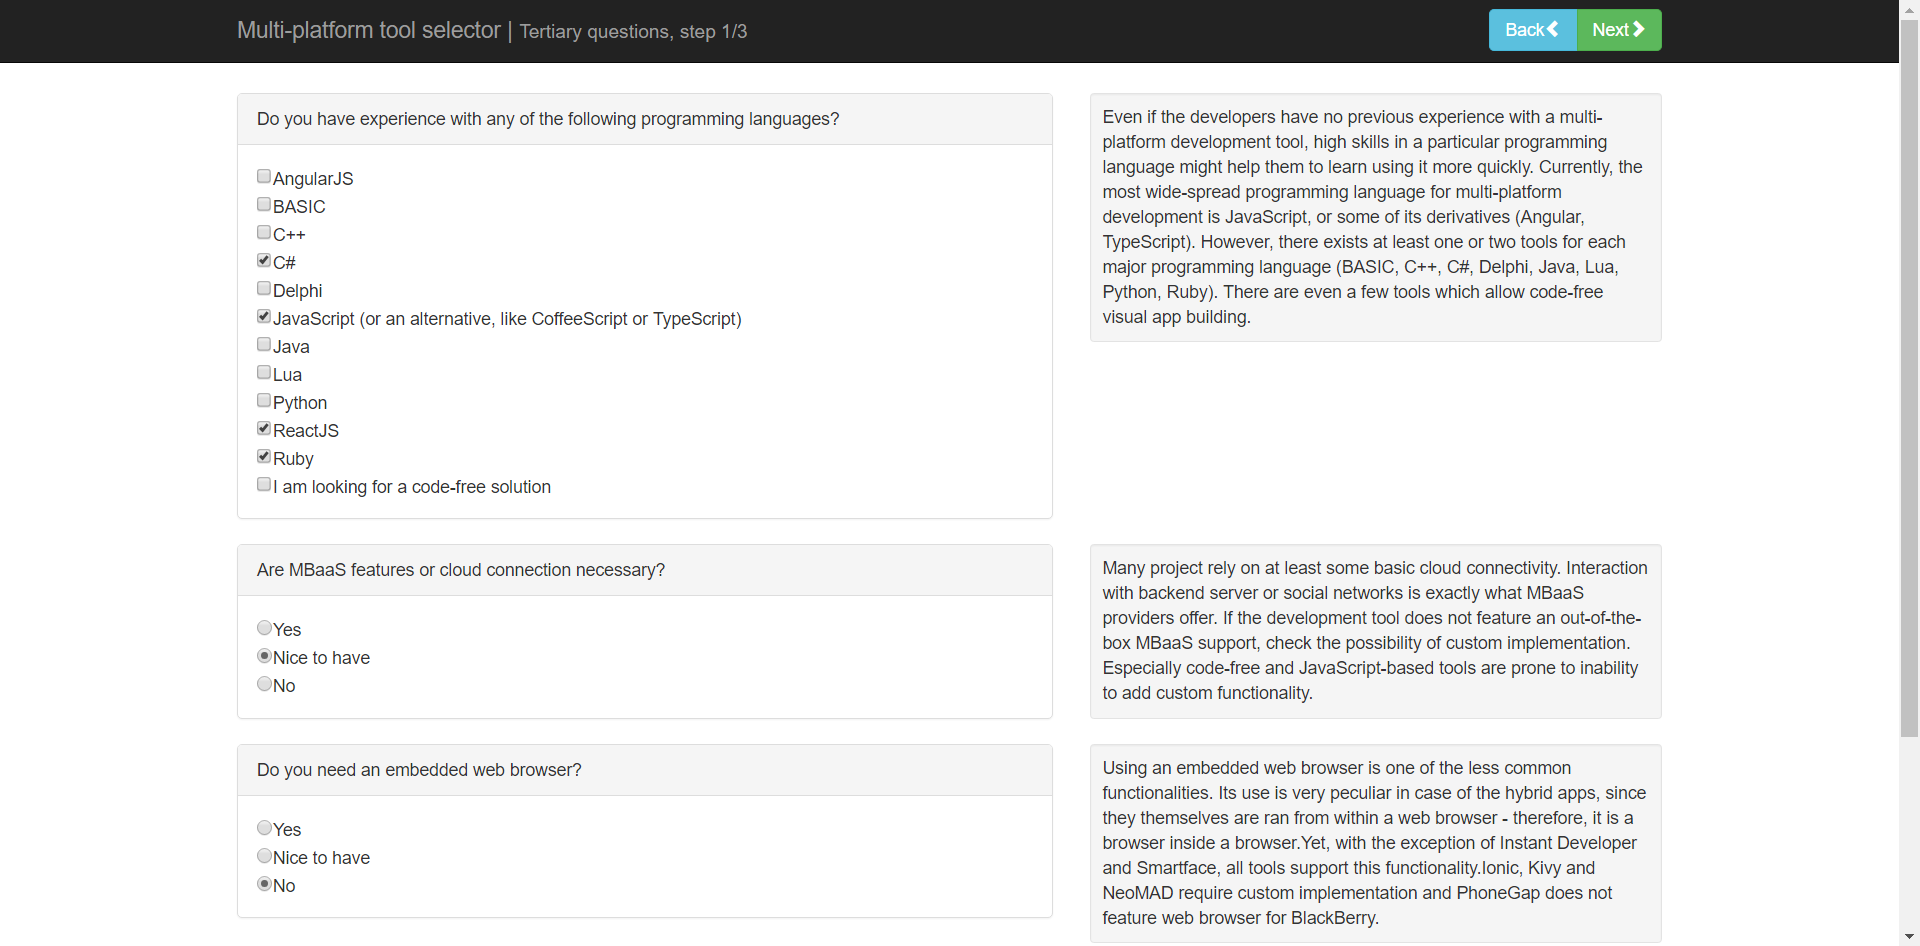
\includegraphics[width=0.8\textwidth]{Figures/morequestions.png}}
	\caption{Tertiary questions page of the methodology web app}
	\label{figure:webMoreQuestions}
\end{figure}

\subsection{Supplementary questions}

This last set of questions does not provide simple answers. However, they may help in investigating the differences between two frameworks that still have similar amount of points, even after passing the first three sets of questions.

\begin{figure}
	\centering\fbox{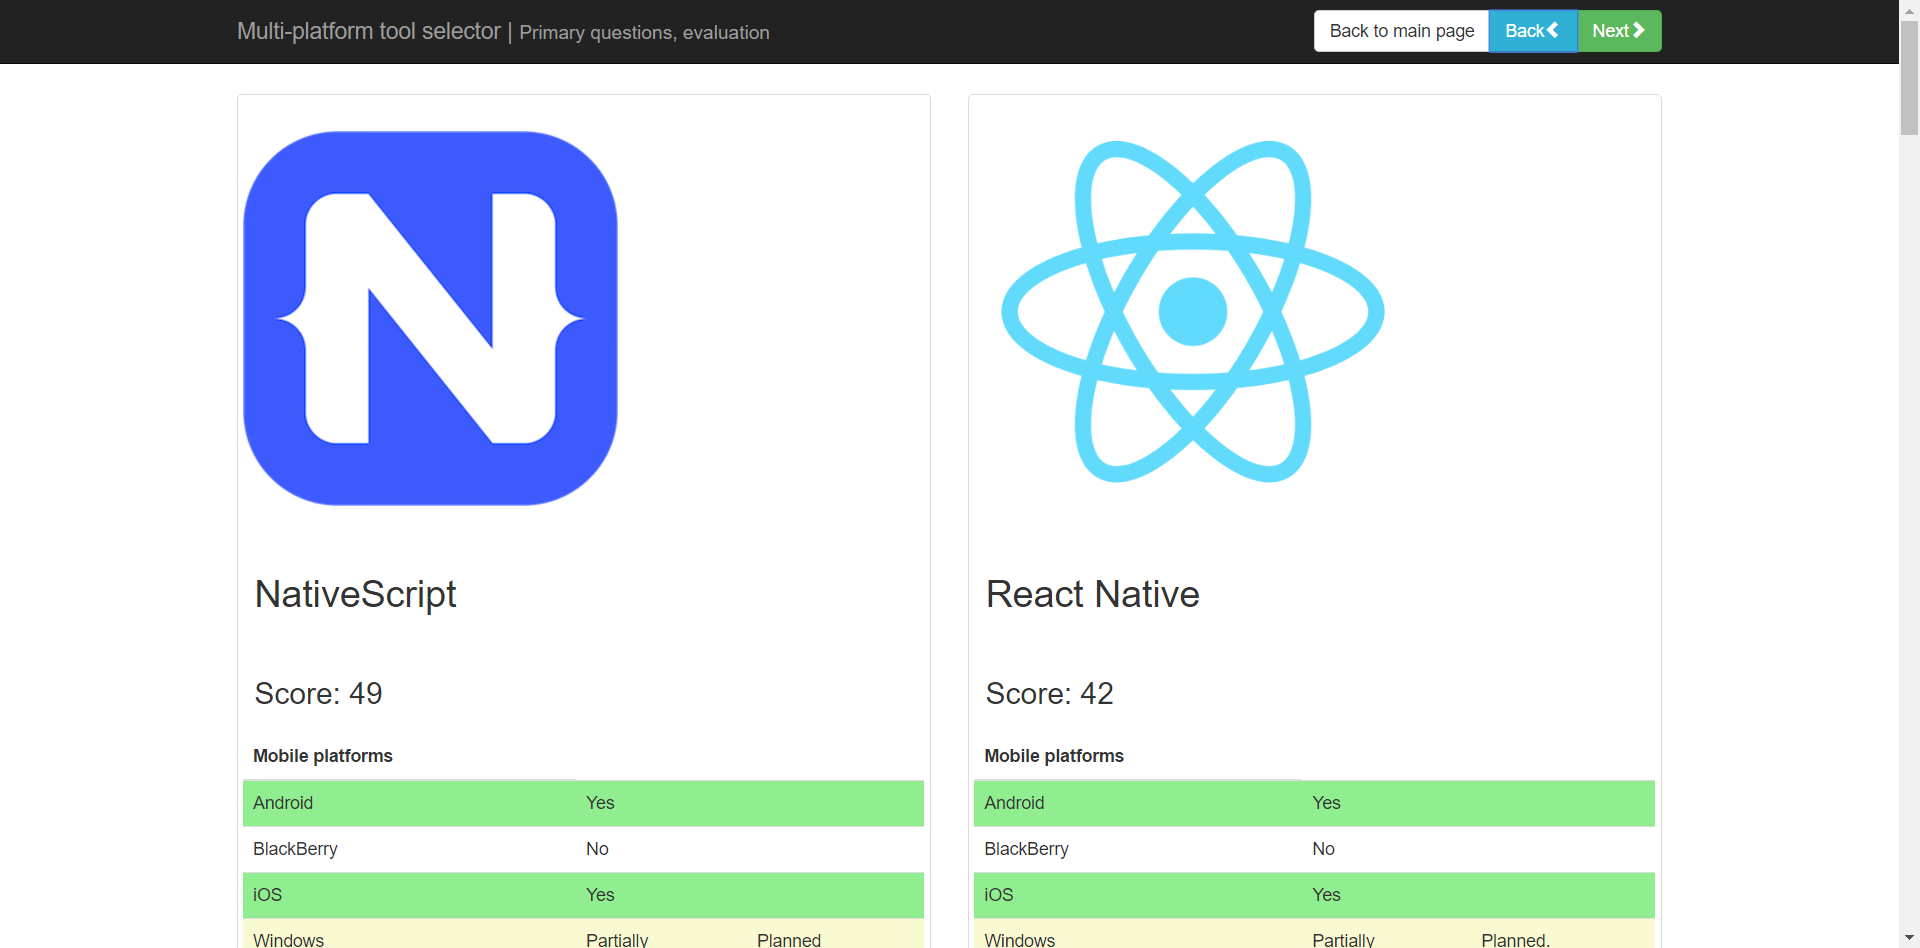
\includegraphics[width=0.8\textwidth]{Figures/evaluation.png}}
	\caption{Evaluation page of the methodology web app}
	\label{figure:webEvaluation}
\end{figure}

\begin{enumerate}
	\item \textbf{Do the developers have experience with a multi-platform development tool? }
	If the answer to this question is yes, then you should consider consulting your development team. Their past experience might be very helpful in resolving the questions with no simple answers, like: What is the learning curve? How long does the development take? What is the performance of the app? Is the development tool buggy? How busy is the developer community?
	
	If the tool used by the developers both satisfies all the customer’s requirements and is advised to be used by the development team itself, it can greatly boost the development speed. They will be familiar with all the pitfalls. Components and design patterns from past projects may be reused. You might find out, that the software licences are still valid and you have enough hardware to test on. All these factors may help to decrease the development time and costs and still satisfying your customer.
	
	\item \textbf{Is there a source of 3rd party libraries? How rich is it? }
	Even if a tool does not implement certain features, it can often be substituted by a 3rd party library. Tools with rich environment of 3rd party libraries often come also with tools enabling easy plugin management. Examples of these can be: Hyperloop by Appcelerator, npm for Apache Cordova and NativeScript plugins, Nuget for Xamarin packages or motion-toolbox for RubyMotion gems.
	
	\item \textbf{Do you have specialists for individual mobile operating systems? }
	As mentioned already multiple times in this thesis, each mobile OS has a different way of handling the app lifecycle. There are differences in communication with the kernel, interactions between apps and handling navigation. There is inconsistency in available APIs, sensors, widgets and varying guidelines to UX and UI design. Some development tools shield you off these differences, focusing on the least common denominator. Others let you leverage the platform-specific features to the full extent.
	
	Having developers specialized for individual operating systems allows you to use the platform-specific approach. While most development tools allow platform-specific overrides, it is default only for RubyMotion and Xamarin (partially also for Appcelerator, React Native and NativeScript). The former approach, where platform-specifics are shielded off (known also as the WORA approach) is used by all other tools, as well as Xamarin.Forms.
	
	\item \textbf{What is the size of the resulting apps? }
	In the early days of Swift, there were many reports that the apps are much larger than apps written in Objective-C\cite{swiftIsBig}. This was due to the fact that Swift was not included in iOS, thus Swift runtine, libraries and API had to be bundled within the app. This is true also of many multi-platform development tools. They often bundle their own runtine, custom libraries, UI styles and APIs together with the application itself, making its installation size bigger. It could be worthwhile to investigate, how large the resulting apps are for individual frameworks.
	
	\item \textbf{What is the learning curve? How long does it take to create a simple app? How long does it take to master the tool?}
	Some programming languages are inherently easier to learn, while others require much greater effort. There are tools which require a lot of initial configuration and settings and then there are frameworks which are fully functional out-of-the-box. Part of the frameworks mentioned in this thesis lie great emphasis on architecture of the code base, yet other allow the developer to patch the code as he/she pleases. Depending on what type of application you wish to achieve, there are tools which are more or less suitable for your project.
	
	\item \textbf{How often is the tool updated? How long does it take to react to a new OS release?}
	As mentioned in the beginning of this thesis, each mobile operating system has already multiple versions. Each version brings new API, increases performance, while may cut off part of redundant functionality from the past. If you app should stay competitive and fresh, it should be prepared for those changes. Try to search how long does it approximately take for a framework to support new OS versions. Some provide 0-day compatibility, while others may require several months to be fully prepared for the new version.
	
	\item \textbf{How comprehensive is the documentation? Are tutorials, courses or books available?}
	To learn something new, each of us needs a source of knowledge. It is almost impossible to learn a new framework without the knowledge how to use it. Thorough documentation is crucial, yet there are tools which provide specification only for basic use cases. However, good courses or books can be even better, quick-starting your project.

	\item \textbf{How buggy is the tool? How are bugs handled?}
	There is no perfect piece of software - bugs are simply everywhere. However, some tools are more stable than others. Very important is also the attitude towards bug solving. Open-source rely on the community support. Some commercial tools are also very open about their bug-solving policy, allowing to track all reported, confirmed and solved bugs. However, there still can be found a few shady examples, which believe that pretending no bug exists will solve the problem.
	
	\item \textbf{What are some prominent apps developed using the tool?}
	If you still are not sure which tool is most suitable for your case, try to look at some apps that were written in that tool. If you find multiple similar apps, it probably means the tool is best suited for your use case.
\end{enumerate}


\section{Methodology verification}
In order to test the methodology out, it has been subjected to several verifications on real projects. 

\subsection{FloLogic}
The first project is called FloLogic. It consists of a mobile application and cloud backend, monitoring and controlling a water valve. The project was started more than a year ago. The original specification required to use Xamarin, because the product owner had an MSDN subscription. Other requirements included:
\begin{enumerate}
	\item Focus on iOS and Android, with later implementation for Windows Phones
	\item Implementation of a Microsoft Azure cloud service, communicating with the mobile app and the water valve
	\item Integration of a highly reliable PUSH notification system
\end{enumerate}

However, during the year several requirements were changed, added or removed. Together with other complications, this resulted in extending a project, originally estimated for 3 months, to more than a year. Changes included 3 different UI designs, starting with platform-agnostic UI to native-like platform-specific and then back to a unified UI. 

The project manager of FloLogic wanted to know, whether Xamarin is still a suitable choice, since the development team was struggling with implementation of individual requirements. He provided the current requirements and compared them against individual sets of questions in this methodology. The same questions were then answered by one of FloLogic developers, to provide a slightly different point of view. The results can be found in table \ref{table:flologicPrimary}.

\begin{table}[!h]
	\centering
	\caption{FloLogic - Primary questions}
	\label{table:flologicPrimary}
	\begin{tabular}{p{5.5cm} | p{3.5cm} | p{3.5cm}}
		\toprule		
		\textbf{Question} &	\textbf{Project manager’s answer} & \textbf{Developer’s answer} \\
		\midrule
		Which mobile operating systems do you want to target? &	Android, iOS & Android, iOS \\
		Which desktop operating systems do you have available for development? & macOS, Windows & Linux, macOS, Windows, web environment \\
		What is the size of your team? & Up to 5 developers & Up to 5 developers \\
		How much are you willing to pay for software licences per developer per year? & \$0 & \$0 \\
		Do you want the app to have native look and feel, or same across individual platforms? & Same & Same \\
		Do you require multithreading? & Yes & Nice to have \\
		Will you use multimedia sensors and APIs (camera, microphone, video and audio player) & No & No \\
		Will you use location sensors (GPS, gyroscope, accelerometer)? & No & No \\
		Do you want to get information about device status? & No & Yes \\
		Will you use a background process? & No & Yes \\
		Will you use PUSH notifications? & Yes & Yes \\
		Do you need to invoke native libraries or create custom plugins? & No & No \\
		Would you like to use app monitoring and get crash analytics? & Nice to have & Nice to have \\		
		\midrule
	\end{tabular}
\end{table}

As the reader can see, the answers of the project manager and developer have differed in a few points, namely:
\begin{itemize}
	\item Desktop operating systems - the developer has stated that even though the company does not currently possess any Linux machines, Ubuntu can be installed on any Windows PC. He mentioned also the possibility to develop in a web environment, which was refused by the project manager due to security considerations.
	\item Multithreading - according to the developer, multithreading is not really necessary, since the only possible point of its use are calls to the cloud server, which can be handled by asynchronous callbacks. The UI is rather static, so slight lags should not impact the user experience. Moreover, the absence of true multithreading can be compensated with web workers in most JavaScript-based tools, or by Lua’s co-routines.
	\item Device status information - the developer expressed the need to check network availability, connection stability, as well as the version of operating system.
	\item Background process - according to the developer, background processes, although unavailable on iOS, are much more reliable on Android, then PUSH notifications. He would therefore prefer a tool allowing the creation of background services.
\end{itemize}

Only 5 tools have managed to pass the primary set of questions according to the project manager’s answers. The developer was more demanding, leaving space only to 4 tools. Table \ref{table:flologicResults1} shows the preliminary results.

\begin{table}[!h]
	\centering
	\caption{FloLogic - Primary questions results}
	\label{table:flologicResults1}
	\begin{tabular}{p{4cm} | p{3cm} | p{3cm} | p{3cm}}
		\toprule		
		\textbf{Tool:} & \textbf{Kivy} & \textbf{Kony} & \textbf{NativeScript} \\
		\midrule
		Manager’s score: & 28 & 42 & 42 \\
		Developer’s score: & 28 & - & 49 \\ 
		\midrule
		\textbf{Tool:} & \textbf{PhoneGap} & \textbf{React Native} & \\
		\midrule
		Manager’s score: & 35 & 35 & \\
		Developer’s score: & 42 & 35 & \\			
		\midrule
	\end{tabular}
\end{table}

As the reader can see, Xamarin was eliminated from further consideration already in the first set of questions. Both Xamarin and Xamarin.Forms target native look and feel of applications. Although it is possible to bypass this with various workarounds (as the FloLogic development team has proven), it takes more than a month, compared to a couple of days done in other tools. 
Let us continue with the second set of questions, which were answered by both the project manager and the developer in table \ref{table:flologicSecondary}.

\begin{table}[!h]
	\centering
	\caption{FloLogic - Secondary questions}
	\label{table:flologicSecondary}
	\begin{tabular}{p{5.5cm} | p{3.5cm} | p{3.5cm}}
		\toprule		
		\textbf{Question} &	\textbf{Project manager’s answer} & \textbf{Developer’s answer} \\
		\midrule
		How complex is your application? & Business-grade & Business-grade \\
		Would you like to use a designer or preview tool? & Nice to have & No \\
		Do you need different layout for tablet and phone? & No & No \\
		Will you use some platform-specific overrides? & No & No \\
		Will you access the file system? & No & No \\
		Do you need any client-side database? & No & No \\
		Will you use Bluetooth, NFC, finger- or barcode scanner? & No & No \\
		Do you require integration with virtual assistants? & No & No \\
		Do you need debugging tools? & Yes & Yes \\
		Will you use unit tests? & Yes & Nice to have \\
		Would you like to use automated UI tests? & Nice to have & No \\
		Would you like to use app profiling? & Nice to have & Yes \\		
		\midrule
	\end{tabular}
\end{table}

Even in the second set some answers differ. The developer was confident enough to create user interfaces purely in code, without the need of a designer tool. Also, the preferences for individual testing techniques differed from the project manager to the developer. After answering the secondary questions, the score look like table \ref{table:flologicResults2}.

\begin{table}[!h]
	\centering
	\caption{FloLogic - Secondary questions results}	
	\label{table:flologicResults2}
	\begin{tabular}{p{4cm} | p{3cm} | p{3cm} | p{3cm}}
		\toprule		
		\textbf{Tool:} & \textbf{Kivy} & \textbf{Kony} & \textbf{NativeScript} \\
		\midrule
		Manager’s score: & 38 & 72 & 62 \\
		Developer’s score: & 38 & - & 64 \\ 
		\midrule
		\textbf{Tool:} & \textbf{PhoneGap} & \textbf{React Native} & \\
		\midrule
		Manager’s score: & 40 & 50 & \\
		Developer’s score: & 42 & 45 & \\			
		\midrule
	\end{tabular}
\end{table}

Already now, the winner is very distinguishable. Kony leads with 72 points, with NativeScript being not that far on the second place. The project manager of FloLogic was familiar with React Native, but both Native Script and Kony were new to him. He wanted to take also tertiary questions in order to see, whether Ract Native comes closer to Kony, or whether the gap widens. Table \ref{table:flologicTertiary} displays the answers for the last set of questions.

\begin{table}[!h]
	\centering
	\caption{FloLogic - Tertiary questions}
	\label{table:flologicTertiary}
	\begin{tabular}{p{9.5cm} | p{3cm}}
		\toprule		
		\textbf{Question} &	\textbf{Project manager’s answer} \\
		\midrule		
		Which programming languages do you have experience with? & AngularJS, C\#, JS, Java, Ruby \\
		Do you require MBaaS features or cloud connection? & Yes \\
		Do you need embedded web browser? & No \\
		Would you like to access the contact list, call or send SMS? & No \\
		Is a testing environment for multiple devices required? & Nice to have \\
		Do you need continuous integration features? & Nice to have \\
		Would you like to test in closed groups? & No \\
		Do you need OpenGL support? & No \\
		Would you like to develop games? & No \\
		Is the app targeted for augmented or virtual reality? & No \\			
		\midrule
	\end{tabular}
\end{table}

\begin{table}[!h]
\centering
\caption{FloLogic - Tertiary questions results}
\label{table:flologicResults3}
	\begin{tabular}{p{4cm} | p{3cm} | p{3cm} | p{3cm}}
		\toprule		
		\textbf{Tool:} & \textbf{Kivy} & \textbf{Kony} & \textbf{NativeScript} \\
		\midrule
		Manager’s score: & 20 & 69 & 59 \\
		\midrule
		\textbf{Tool:} & \textbf{PhoneGap} & \textbf{React Native} & \\
		\midrule
		Manager’s score: & 28 & 38 & \\		
		\midrule
	\end{tabular}
\end{table}

The manager was surprised with the results and displayed deep interest in the Kony framework. He expressed himself that he would discuss the results with the product owner. However, he added he is rather sceptical about changing the framework after more than a year of development and starting from scratch.

\subsection{Project W}

The next project belongs to an indie startup which tries to fill the "App gap" in Windows market. They realize that Windows is not particularly strong in the mobile field, but thanks to the concepts of Universal Windows Platform they would like to create an app that runs on smartphones, tablets and desktops as well. Although this methodology does not focus on multi-platform desktop development tools, some frameworks mentioned in this thesis allow it as well.

The goal of Project W is to create an app that helps the user to track his/her daily water intake. Unlike similar apps, this app calculates the required water intake dynamically based on local weather, user statistics and data from other health-tracking apps the user might have installed. The answers to the first set of questions can be found in table \ref{table:wPrimary}.

\begin{table}[!h]
	\centering
	\caption{Project W - Primary questions}
	\label{table:wPrimary}
	\begin{tabular}{p{9cm} | p{4.5cm}}
		\toprule		
		\textbf{Question} &	\textbf{Answer}\\
		\midrule
		Which mobile operating systems do you want to target? &	Android, iOS, Windows \\
		Which desktop operating systems do you have available for development? & Windows (maybe macOS) \\
		Do you require iOS builds without the need of a Mac? & Nice to have \\
		What is the size of your team? & Indie \\
		How much are you willing to pay for software licences per developer per year? & \$0 \\
		Do you want the app to have native look and feel, or same across individual platforms? & Native look and feel \\
		Do you want to code a single UI layer for all operating systems, or a custom layer for each mobile OS? & Single \\
		Do you require multithreading? & Nice to have \\
		Will you use multimedia sensors and APIs (camera, microphone, video and audio player) & No  \\
		Will you use location sensors (GPS, gyroscope, accelerometer)? & GPS \\
		Do you want to get information about device status? & Yes \\
		Will you use a background process? & No \\
		Will you use PUSH notifications? & Yes \\
		Do you need to invoke native libraries or create custom plugins? & No \\
		Would you like to use app monitoring and get crash analytics? & Nice to have \\		
		\midrule
	\end{tabular}
\end{table}

The startup has quite limited resources. Although they would like to create apps for iOS, they currently do not own a Mac. They had planned to buy one, but as soon as they heard some tools allow iOS builds without a Mac, they showed deep interest for this possibility. Even with this limitation, 7 frameworks have passed the primary questions.

\begin{table}[!h]
	\centering
	\caption{Project W - Primary questions results}
	\label{table:wResults1}
	\begin{tabular}{p{4cm} | p{3cm} | p{3cm} | p{3cm}}
		\toprule		
		\textbf{Tool:} & \textbf{Embarcadero} & \textbf{Ionic} & \textbf{Monaca} \\ 
		\midrule
		Score: & 56 & 42 & 42 \\ 
		\midrule
		\textbf{Tool:} & \textbf{NativeScript} & \textbf{React Native} & \textbf{Tabris.js} \\
		\midrule
		Score: & 42 & 28 & 56 \\
		\midrule
		\textbf{Tool:}& \textbf{Xamarin} & & \\	
		\midrule
		Score: & 49 & & \\	
		\midrule
	\end{tabular}
\end{table}

We can see that all selected frameworks have fairly equal score (except of React Native), with Embarcadero and Tabris.js slightly standing out. It is interesting though that the filtered tools contain all types of approaches - hybrid, interpreted and even cross-platform. In this case, passing another set of questions is absolutely necessary.

\begin{table}[!h]
	\centering
	\caption{Project W - Secondary questions}
	\label{table:wSecondary}
	\begin{tabular}{p{7.5cm} | p{5cm}}
		\toprule		
		\textbf{Question} &	\textbf{Answer} \\
		\midrule
		How complex is your application? & Native-like \\
		Would you like to use a designer or preview tool? & Nice to have \\
		Do you need different layout for tablet and phone? & Yes \\
		Will you use some platform-specific overrides? & No \\
		Will you access the file system? & No \\
		Do you need any client-side database? & SQLite or Realm \\
		Will you use Bluetooth, NFC, finger- or barcode scanner? & Barcode scanner \\
		Do you require integration with virtual assistants? & No \\
		Do you need debugging tools? & Yes \\
		Will you use unit tests? & Nice to have \\
		Would you like to use automated UI tests? & Nice to have \\
		Would you like to use app profiling? & No \\		
		\midrule
	\end{tabular}
\end{table}

Although the Project W application will be rather simple considering the UI, it will have a lot of backend functionality, synchronization with other apps and API calls - thus it was categorized as a native-like app. The developers also wanted to use a built-in barcode scanner, so the app could scan bottled waters, juices, etc. With these additional requirements, the score table has changed considerably.

\begin{table}[!h]
	\centering
	\caption{Project W - Secondary questions results}
	\label{table:wResults2}
	\begin{tabular}{p{4cm} | p{3cm} | p{3cm} | p{3cm}}
		\toprule		
		\textbf{Tool:} & \textbf{Embarcadero} & \textbf{Ionic} & \textbf{Monaca} \\ 
		\midrule
		Score: & 86 & 72 & 57 \\ 
		\midrule
		\textbf{Tool:} & \textbf{NativeScript} & \textbf{React Native} & \textbf{Tabris.js} \\
		\midrule
		Score: & 52 & 48 & 66 \\
		\midrule
		\textbf{Tool:}& \textbf{Xamarin} & & \\	
		\midrule
		Score: & 94 & & \\	
		\midrule
	\end{tabular}
\end{table}

Embarcadero is still at the forefront, but Xamarin surpassed it together with Tabris.js, which is now in the 4th place. React Native, Monaca and NativeScript seem to be insufficient for this app. The developers were curious, whether the last set of questions will have similarly dramatic effect on the score of individual frameworks.

\begin{table}[!h]
	\centering
	\caption{Project W - Tertiary questions}
	\label{table:wTertiary}
	\begin{tabular}{p{7.5cm} | p{5cm}}
		\toprule		
		\textbf{Question} &	\textbf{Answer} \\
		\midrule		
		Which programming languages do you have experience with? & C\#, JavaScript \\
		Do you require MBaaS features or cloud connection? & Yes \\
		Do you need embedded web browser? & No \\
		Would you like to access the contact list, call or send SMS? & No \\
		Is a testing environment for multiple devices required? & No \\
		Do you need continuous integration features? & Nice to have \\
		Would you like to test in closed groups? & Yes \\
		Do you need OpenGL support? & No \\
		Would you like to develop games? & No \\
		Is the app targeted for augmented or virtual reality? & No \\			
		\midrule
	\end{tabular}
\end{table}

\begin{table}[!h]
	\centering
	\caption{Project W - Tertiary questions results}
	\label{table:wResults3}
	\begin{tabular}{p{4cm} | p{3cm} | p{3cm} | p{3cm}}
		\toprule		
		\textbf{Tool:} & \textbf{Embarcadero} & \textbf{Ionic} & \textbf{Monaca} \\ 
		\midrule
		Score: & 80 & 72 & 60 \\ 
		\midrule
		\textbf{Tool:} & \textbf{NativeScript} & \textbf{React Native} & \textbf{Tabris.js} \\
		\midrule
		Score: & 52 & 48 & 63 \\
		\midrule
		\textbf{Tool:}& \textbf{Xamarin} & & \\	
		\midrule
		Score: & 100 & & \\	
		\midrule
	\end{tabular}
\end{table}

As we can see, Embarcadero has lost 6 points, while Xamarin has only strengthened its position at exactly 100 points. It is clear now that Xamarin is the most suitable framework for Project W. The developers have admitted they heard of Xamarin a lot and considered it even before passing through this methodology. With Xamarin, they can develop not only for mobile, but also Windows desktop (with Universal Windows Platform) and Mac (with Xamarin.Mac). The only platform Xamarin does not target is Linux.

\subsection{Sensus}

The last tested project is called Sensus. This is again a Xamarin project targeted for Android and Windows. The project is extension to an existing family of .NET projects for web and desktop environments. Xamarin was chosen in the hope to re-use some common libraries. In Sensus, high importanse is put on bluetooth and QR code scanner functionality. Tables \ref{table:sensusPrimary} - \ref{table:sensusTertiary} show the scrum master's answers to all three sets of questions.

\begin{table}[!h]
	\centering
	\caption{Sensus - Primary questions}
	\label{table:sensusPrimary}
	\begin{tabular}{p{7.5cm} | p{5cm}}
		\toprule		
		\textbf{Question} &	\textbf{Answer}\\
		\midrule
		Which mobile operating systems do you want to target? &	Android, Windows \\
		Which desktop operating systems do you have available for development? & Linux, Windows \\
		What is the size of your team? & Up to 10 developers \\
		How much are you willing to pay for software licences per developer per year? & \$500 \\
		Do you want the app to have native look and feel, or same across individual platforms? & Same \\
		Do you require multithreading? & Yes \\
		Will you use multimedia sensors and APIs (camera, microphone, video and audio player) & Camera  \\
		Will you use location sensors (GPS, gyroscope, accelerometer)? & GPS \\
		Do you want to get information about device status? & Nice to have \\
		Will you use a background process? & No \\
		Will you use PUSH notifications? & No \\
		Do you need to invoke native libraries or create custom plugins? & No \\
		Would you like to use app monitoring and get crash analytics? & No \\		
		\midrule
	\end{tabular}
\end{table}

\begin{table}[!h]
	\centering
	\caption{Sensus - Secondary questions}
	\label{table:sensusSecondary}
	\begin{tabular}{p{7.5cm} | p{5cm}}
		\toprule		
		\textbf{Question} &	\textbf{Answer} \\
		\midrule
		How complex is your application? & Business-grade \\
		Would you like to use a designer or preview tool? & No \\
		Do you need different layout for tablet and phone? & Nice to have \\
		Will you use some platform-specific overrides? & Yes \\
		Will you access the file system? & No \\
		Do you need any client-side database? & SQLite \\
		Will you use Bluetooth, NFC, finger- or barcode scanner? & Bluetooth, QR scanner \\
		Do you require integration with virtual assistants? & No \\
		Do you need debugging tools? & Yes \\
		Will you use unit tests? & Yes \\
		Would you like to use automated UI tests? & Yes \\
		Would you like to use app profiling? & Nice to have \\		
		\midrule
	\end{tabular}
\end{table}

\begin{table}[!h]
	\centering
	\caption{Sensus - Tertiary questions}
	\label{table:sensusTertiary}
	\begin{tabular}{p{9.5cm} | p{3cm}}
		\toprule		
		\textbf{Question} &	\textbf{Answer} \\
		\midrule		
		Which programming languages do you have experience with? & AngularJS, C\#, JS, Java \\
		Do you require MBaaS features or cloud connection? & No \\
		Do you need embedded web browser? & No \\
		Would you like to access the contact list, call or send SMS? & No \\
		Is a testing environment for multiple devices required? & Nice to have \\
		Do you need continuous integration features? & Nice to have \\
		Would you like to test in closed groups? & No \\
		Do you need OpenGL support? & No \\
		Would you like to develop games? & No \\
		Is the app targeted for augmented or virtual reality? & No \\			
		\midrule
	\end{tabular}
\end{table}

As the reader will notice, the same set of frameworks which satisfied the requirements of FloLogic were selected also for Sensus. This is remarkable, since the answers were substantially different. However, while Kony was the most suitable framework for FloLogic, NativeScript leads in case of Sensus, with PhoneGap being second.

\begin{table}[!h]
	\centering
	\caption{Sensus - Questions results}
	\label{table:sensusResults}
	\begin{tabular}{p{4cm} | p{3cm} | p{3cm} | p{3cm}}
		\toprule		
		\textbf{Tool:} & \textbf{Kivy} & \textbf{Kony} & \textbf{NativeScript} \\ 
		\midrule
		Score: & 45 & 55 & 80 \\ 
		\midrule
		\textbf{Tool:} & \textbf{PhoneGap} & \textbf{React Native} & \\
		\midrule
		Score: & 68 & 59 & \\
		\midrule
	\end{tabular}
\end{table}

The scrum master was very surprised why Xamarin was not even listed among the selected frameworks. Under closer inspection, we can see it was removed by the requirement of having the same look and feel on all targeted platforms.

The scrum master confirmed the development team struggled with this issue for a long time. However, he noted that they eventually managed to achieve this goal. Moreover, the ability to re-use existing C\# libraries outweighted the negatives of implementing custom UI layer. The scrum master suggested the condition of having the same UI across platforms to be less strict. He also pointed out the methodology does not take into account existing code libraries, which might be a decisive factor for some projects. Other than that, he rated the methodology as comprehensive enough and stated that the resulting frameworks might be more suitable for the Sensus project, if there were no custom C\# libraries.

\subsection{Methodology feedback}

After passing the methodology questions, each person was asked to give feedback to the methodology itself.

The project manager of FloLogic assessed the metholody as very comprehensive, clear and easy to use. He admitted that Xamarin may not be the optimal framework for FloLogic's use case. Both Kony and NativeScript, which scored the highest in his answers, were new to hime. He suggested adding several more questions, like:

\begin{itemize}
	\item Do the developers have previous experience with a tool?
	\item How long does it take to learn and master the framework?
	\item How reliable is the tool? How many bugs does it have?
	\item How often is it updated?
\end{itemize}

After being informed that all of these questions are part of the supplementary questions set, he expressed himself as being very satisfied with the methodology.

The FloLogic developer was also quick to agree with Xamarin not being suitable for the project. He has heard of NativeScript never before, but he knew React Native's Facebook Messanger application. React Native was the second most suitable framework in his answers. He expressed his concerns about this framework, being very performance-demanding and thus slow on older phones. After a short benchmark research, which revealed that NativeScript should perform better than React Native, but not as good as Xamarin, he suggested increasing the importance of performance factors in the methodology. He also wanted to add a question about the comprehensivness of documentation. However, this question is already part of the supplementary set.

The developer of Project W has also complimented the methodology as being very thorough and well-structured. She has confirmed planning to use Xamarin for their project, which also came out of the methodology with the highest score. Although she was disappointed a little, that Xamarin required a Mac to build iOS applications, she expressed that it makes the most sense to use a C\#-based framework, since they want to target Windows Phone primarily, anyway.

In case of the Sensus project, it's scrum master confirmed as well that the team was struggling a lot with providing platform-agnostic UI, while using Xamarin. He assessed the questions as being very good and the result - NativeScript or PhoneGap - as being fair enough. However, he stressed the importance of existing libraries re-use, which is not taken into consideration in the methodology. He suggested that some questions should be less decisive (the possibility of creating a platform-specific or platform-agnostic UI), while others should be put more into the forefront (code re-use and integration with existing libraries). He wanted to know, whether there are no other frameworks using C\#. When informed of InstantDeveloper, he pointed out that this might have been a better choice.


\section{Conclusion}

In this thesis we have successfully designed and created a complex methodology for selecting the most suitable development tool for mobile multi-platform projects. The methodology was tested on a series of real-world projects. Gathered feedback has evaluated the methodology as comprehensive, well-structured, producing solid and reliable results. 

The methodology was created by fulfilling several partial goals. At first, we have analyzed the current market, selecting relevant mobile platforms. Those platforms were then further used to limit the number of frameworks described in this thesis. Studied development tools had to also pass the criteria of being general-purpose, not being a game engine or a web framework. This has resulted in a total of 25 multi-platform frameworks.

Three most popular representatives of these frameworks, Apache Cordova, React Native and Xamarin, were then closely tested by implementing 6 common use-case scenarios in each of them. The findings from said practical implementations were eventually combined with researched theoretical knowledge, to produce the methodology itself. The web application representing the methodology will be used not only by SDE Software Solutions, but will be made public for anyone to use.

The main contribution of this thesis and, particularly, the methodology is its generality. Because of the large number of studied development tools, the methodology can be applied to any general-purpose mobile development. Unlike similar academic works, which compare only a handful of frameworks, the methodological steps from this thesis will be valid also in the near future, with minimal fine tuning.

This fine tuning may include re-assessing the importance of individual questions or adding new criteria and new frameworks, which may be developed in the future. Frameworks and requirements that will cease to exist may be removed from the methodology, or made less important. Additionaly, similar methodologies may be developed, focusing on game engines, web application frameworks or single-purpose enterprise tools.


\begin{thebibliography}{99}	
	%A
	\bibitem{apacheCordova} WARGO, John M. \textit{Apache Cordova 3 Programming}. First release. New Jersey 07458: Pearson Education, 2013. ISBN 978-0-321-95736-8.
	\bibitem{rajTolety} RAJ, R a SB TOLETY. A study on approaches to build cross-platform mobile applications and criteria to select appropriate approach. \textit{2012 Annual IEEE India Conference (INDICON)}. 2012, 625–9.
	\bibitem{awsDeviceFarm} \textit{AWS Device Farm} [online]. [cit. 2017-03-11]. Available at: https://aws.amazon.com/device-farm/	
	%B
	\bibitem{bitbar} \textit{Bitbar}. [online]. [cit. 2017-03-11]. Available at: http://bitbar.com/testing/	
	\bibitem{wikiBBWorld} BlackBerry World. In: \textit{Wikipedia: the free encyclopedia} [online]. San Francisco (CA): Wikimedia Foundation, 2001- [cit. 2017-03-10]. Available at: https://en.wikipedia.org/wiki/BlackBerry\_World\#Milestones
	\bibitem{blogsWindows8to10} Bring your Windows Phone Silverlight apps to Windows Runtime XAML; prepare for universal app development in Windows 10. \textit{Windows blogs} [online]. [cit. 2017-03-10]. Available at: https://blogs.windows.com/buildingapps/2014/12/17/bring-your-windows-phone-silverlight-apps-to-windows-runtime-xaml-prepare-for-universal-app-development-in-windows-10/
	%C
	\bibitem{cordovaVsCodename} COMPARING PHONEGAP/CORDOVA AND CODENAME ONE. \textit{Codename One} [online]. [cit. 2017-02-26]. Available at: https://www.codenameone.com/blog/comparing-phonegap-cordova-and-codename-one.html
	\bibitem{rhoMobile} PALMIERI, Manuel, Inderjeet SINGH a Antonio CINCCHETTI. \textit{Comparison of Cross-Platform Mobile Development Tools} [online]. [cit. 2017-03-18]. Available at: https://pdfs.semanticscholar.org/be08/83eab3d3d6eb10c4ff1189163f6453254da1.pdf
	\bibitem{wikiCrossPlatform} Cross-platform. In: \textit{Wikipedia: the free encyclopedia} [online]. San Francisco (CA): Wikimedia Foundation, 2001- [cit. 2017-03-10]. Available at: https://en.wikipedia.org/wiki/Cross-platform
	\bibitem{aComparativeStudy}DE ANDRADE, Paulo R. M. a Adriano B. ALBUQUERQUE. \textit{Cross Platform App: A comparative study} [online]. Postgraduate program in applied information University of Fortaleza - UNIFOR Fortaleza - CE, Brazil, 2015 [cit. 2017-02-19].
	\bibitem{uppsala} FURUSKOG, Martin a Stuart WEMYSS. \textit{Cross-platform development of smartphone applications: An evaluation of React Native} [online]. Uppsala Universitet, 2016 [cit. 2017-02-19]. In: https://uu.diva-portal.org/smash/get/diva2:948617/FULLTEXT01.pdf
	\bibitem{aarhus}NIELSEN, Bobby. \textit{Cross Platform Mobile Development} [online]. Department of Computer Science, University of Aarhus, 2015 [cit. 2017-02-19]. In: https://pdfs.semanticscholar.org/de11/7b518d31ebcad7a864f9b16d1bcd53365d6a.pdf
	\bibitem{codenameOneNaive} CROSS PLATFORM MOBILE STILL BETTER THAN NAIVE IN AGE OF FLAT DESIGN. \textit{Codename One} [online]. [cit. 2017-03-10]. Available at: https://www.codenameone.com/blog/cross-platform-mobile-still-better-than-native-in-age-of-flat-design.html
	\bibitem{cptBenchmarking2014} \textit{Cross-Platform Tool Benchmarking 2014} [online]. [cit. 2017-02-19]. In: http://www.research2guidance.com/r2g/Cross-Platform-Tool-Benchmarking-Report-2014.pdf
	%D
	\bibitem{definingTelerik} Defining a New Breed of Cross-Platform Mobile Apps. \textit{Telerik} [online]. 2015 [cit. 2017-02-19]. In: http://developer.telerik.com/featured/defining-a-new-breed-of-cross-platform-mobile-apps/
	\bibitem{idcDetachableTablets} Detachable Tablets Set To Grow From 8\% of the Tablet Market in 2015 to 30\% in 2020, According to IDC. \textit{IDC} [online]. [cit. 2017-03-10]. Available at: http://www.idc.com/getdoc.jsp?containerId=prUS41072516
	\bibitem{betanewsWinRevenue} Developers earn more on Windows Phone than Android or iOS. \textit{Betanews} [online]. [cit. 2017-03-10]. Available at: http://betanews.com/2016/02/29/windows-phone-developer-revenue/
	%E
	\bibitem{evaluationOfCP} FRIBERG, Joy. \textit{Evaluation of cross-platform development for mobile devices} [online]. Department of Computer and Information Science , Linköpings universitet, 2014 [cit. 2017-02-19]. In: https://www.diva-portal.org/smash/get/diva2:691708/FULLTEXT01.pdf	
	%F
	\bibitem{firebase} \textit{Firebase Test Lab for Android} [online]. [cit. 2017-03-11]. Available at: https://firebase.google.com/docs/test-lab/	
	%G
	\bibitem{gartner} \textit{Gartner} [online]. [cit. 2017-03-11]. Available at: http://www.gartner.com/technology/home.jsp
	\bibitem{ionicGetStarted} Get started with Ionic Framework. \textit{Ionic} [online]. [cit. 2017-02-26]. Available at: http://ionicframework.com/getting-started/
	%H
	\bibitem{lifehackerRevenues} How Much Do Mobile Developers Make Per App? \textit{Lifehacker} [online]. [cit. 2017-03-10]. Available at: http://www.lifehacker.com.au/2016/03/how-much-do-mobile-developers-make-per-app/
	%I
	\bibitem{appcodaiPad} IOS Programming Tutorial: Creating a Universal App. \textit{Appcoda} [online]. [cit. 2017-03-10]. Available at: http://www.appcoda.com/ios-univeral-app-tutorial/
	\bibitem{iosAndroidStore} IOS vs Android Market Share \& Revenue: One Win for Each App Store in 2015. \textit{Latin Post} [online]. [cit. 2017-03-10]. Available at: http://www.latinpost.com/articles/110519/20160121/ios-vs-android-market-share-revenue-one-win-for-each-app-store-in-2015.htm
	%J
	%K
	%L
	%M
	\bibitem{worldBank} Mobile cellular subscriptions (per 100 people). \textit{The World Bank} [online]. [cit. 2017-03-10]. Available at: http://data.worldbank.org/indicator/IT.CEL.SETS.P2?view=map\&year=2000
	\bibitem{smutny}SMUTNÝ, P. \textit{Mobile development tools and cross-platform solutions.} 13th International Carpathian Control Conference (ICCC). 2012, 653–6.
	\bibitem{xamarin} SHACKLES, Greg. \textit{Mobile development with C\#}. Sebastopol, CA: O'Reilly, c2012. ISBN 978-1-449-32023-2.
	\bibitem{wikiSmartphoneSales} Mobile operating system. In: \textit{Wikipedia: the free encyclopedia} [online]. San Francisco (CA): Wikimedia Foundation, 2001- [cit. 2017-03-11]. Available at: https://en.wikipedia.org/wiki/Mobile\_operating\_system\#By\_operating\_system
	\bibitem{mosMarketShare} Mobile/Tablet Operating System Market Share. \textit{NetMarketShare} [online]. [cit. 2017-03-10]. Available at: https://www.netmarketshare.com/operating-system-market-share.aspx?qprid=8\&qpcustomd=1
	%N
	\bibitem{nativeScriptWinSupport} NativeScript Runtime Preview for Windows 10. \textit{NativeScript} [online]. [cit. 2017-03-10]. Available at: https://www.nativescript.org/blog/nativescript-runtime-preview-for-windows-10
	\bibitem{iosUsersPay} New Report Shows iOS Users Spend Money, Like to Check Weather. \textit{The Mac Observer} [online]. [cit. 2017-03-10]. Available at: https://www.macobserver.com/tmo/article/new\_report\_shows\_ios\_users\_spend\_money \_like\_to\_check\_weather
	\bibitem{appsInStores} Number of apps available in leading app stores as of June 2016. \textit{Statista} [online]. [cit. 2017-03-10]. Available at: https://www.statista.com/statistics/276623/number-of-apps-available-in-leading-app-stores/
	\bibitem{noOfSmartphones} Number of smartphone users worldwide from 2014 to 2020 (in billions). \textit{Statista} [online]. [cit. 2017-03-10]. Available at: http://www.statista.com/statistics/330695/number-of-smartphone-users-worldwide/
	%O
	\bibitem{bgrBBRevenues} One chart shows why BlackBerry 10 has struggled to attract developers. \textit{BGR} [online]. [cit. 2017-03-10]. Available at: http://bgr.com/2013/11/26/blackberry-10-developer-revenues/
	%P
	\bibitem{xamarinPlugins} Plugins for Xamarin and Windows Projects. \textit{GitHub} [online]. [cit. 2017-03-11]. Available at: https://github.com/jamesmontemagno/Xamarin.Plugins
	%Q
	%R
	\bibitem{reactNativeCamera} React-native-camera. \textit{GitHub} [online]. [cit. 2017-03-11]. Available at: https://github.com/lwansbrough/react-native-camera
	\bibitem{npmReactNativeWindows} React-native-windows. \textit{Npm} [online]. [cit. 2017-02-26]. Available at: https://www.npmjs.com/package/react-native-windows
	\bibitem{reactNativeWinSupport} React Native on the Universal Windows Platform. \textit{Windows blogs} [online]. [cit. 2017-03-10]. Available at: https://blogs.windows.com/buildingapps/2016/04/13/react-native-on-the-universal-windows-platform/\#cFzRYQ06Y3lx1Yo8.97
	\bibitem{devEconomics} Reports. \textit{Developer Economics} [online]. [cit. 2017-03-10]. Available at: https://www.developereconomics.com/reports/
	%S
	\bibitem{kantarOSSales} Smartphone OS sales market share. \textit{Kantar Worldpanel} [online]. [cit. 2017-03-11]. Available at: https://www.kantarworldpanel.com/global/smartphone-os-market-share/
	\bibitem{androidTablet} Supporting Tablets and Handsets. \textit{Android Developer} [online]. [cit. 2017-03-10]. Available at: https://developer.android.com/guide/practices/tablets-and-handsets.html
	\bibitem{ribeiroDaSilva} DA SILVA, Ribeiro A. \textit{Survey on cross-platforms and languages for mobile apps}. 2012 eighth international conference on the Quality of Information and Communications Technology (QUATIC). \textbf{2012}, 255-60.
	\bibitem{swiftIsBig} Swift Embedded Runtime Library Increases App Size. \textit{Doing things the hard way…: But only once} [online]. [cit. 2017-03-11]. Available at: http://blog.diogot.com/blog/2014/09/29/swift-embedded-runtime-library-increases-app-size/
	%T
	\bibitem{tabletMarketShare} Tablet operating systems' market share worldwide from 2013 to 2020. \textit{Statista} [online]. [cit. 2017-03-10]. Available at: https://www.statista.com/statistics/272446/global-market-share-held-by-tablet-operating-systems/
	\bibitem{taxonomyCP}EL-KASSAS, Wafaa S., Bassem A. ABDULLAH, Ahmed H. YOUSEF a Ayman M. WAHBA. \textit{Taxonomy of Cross-Platform Mobile Applications Development Approaches} [online]. Department of Computer and Systems Engineering, Faculty of Engineering, Ain Shams University, Egypt, 2015 [cit. 2017-02-19]. In: http://www.sciencedirect.com/science/article/pii/S2090447915001276
	\bibitem{testObject} \textit{TestObject} [online]. [cit. 2017-03-11]. Available at: https://testobject.com/
		
	%U
	%V
	%W
	\bibitem{microsoftContinuum} Welcome to Continuum for phone. \textit{Microsoft Support} [online]. [cit. 2017-03-10]. Available at: https://support.microsoft.com/en-us/help/17280/windows-10-mobile-continuum	
	\bibitem{windowsDevCenter} Windows. \textit{Windows Dev Center} [online]. [cit. 2017-03-10]. Available at: https://developer.microsoft.com/en-us/windows
	\bibitem{wikiWindowsMobile} Windows 10 Mobile. In: \textit{Wikipedia: the free encyclopedia} [online]. San Francisco (CA): Wikimedia Foundation, 2001- [cit. 2017-03-10]. Available at: https://en.wikipedia.org/wiki/Windows\_10\_Mobile					
	\bibitem{codenameOneWinSupport} WINDOWS PHONE 8.1 \& UWP SUPPORT. \textit{Codename One} [online]. [cit. 2017-03-10]. Available at: https://www.codenameone.com/blog/windows-phone-8-1-uwp-support.html
	\bibitem{idcTabletShare} Worldwide Tablet Market Expected to Rebound in 2018 as Windows Opens Doors for Growth and iPads Come Out of a Slump, According to IDC. \textit{IDC} [online]. [cit. 2017-03-10]. Available at: https://www.idc.com/getdoc.jsp?containerId=prUS41699516
	%X
	%Y
	%Z
\end{thebibliography}



\appendix
\section{Overview of studied frameworks}

\subsection{Alpha Anywhere}

\begin{table}[!h]
	\centering
	\caption{Alpha Anywhere}
	\begin{tabular}{p{.33\textwidth} | p{.33\textwidth} | p{.34\textwidth}}
		\toprule		
		\textbf{Framework} & \textbf{Alpha Anywhere} & https://www.alphasoftware.com/mobile-app-development/ \\
		\midrule
		\textbf{Approach} & Hybrid & \\			
		\midrule	
		\textbf{Most suitable for} & Small simple apps, prototyping & \\
		\midrule
		\textbf{Popularity} & Average & \\			
		\midrule
		\textbf{Available APIs} & Audio, video, device status, push notifications, file system, app properties & \\			
		\midrule
		\textbf{Supported assistants} & None & \\			
		\midrule
		\textbf{Augmented or virtual reality} & No & \\			
		\midrule
		\textbf{Background services or processes} & No & \\			
		\midrule
		\textbf{Databases} & SQLite & \\			
		\midrule
		\textbf{Can be developed in} & Web environmnet & Does not require Mac for iOS builds. \\			
		\midrule
		\textbf{Game development} & No & \\			
		\midrule
		\textbf{Invoke native libraries} & No & \\			
		\midrule
		\textbf{Programming languages} & Code-free, JavaScript & \\			
		\midrule
		\textbf{Can build apps for} & Android, iOS & \\			
		\midrule
		\textbf{MBaaS} & Yes & \\			
		\midrule
		\textbf{Multithreading} & Partially & Available with script thread processes. \\			
		\midrule
		\textbf{OpenGL} & No & \\			
		\midrule
		\textbf{Platform-specific overrides} & No & \\			
		\midrule
		\textbf{Approximate prices (per developer per year)} & Indie or up to 5 developers - \$ 1499. Up to 25 developers - \$2499. & Enterprise prices on demand. \\			
		\midrule
		\textbf{Supported sensors} & Camera, microphone, geolocation, accelerometer, gyroscope, fingerprint and barcode scanners & \\			
		\midrule
	\end{tabular}
\end{table}
	
\begin{table}[!h]
	\centering
	\caption{Alpha Anywhere ctd}
	\begin{tabular}{p{.33\textwidth} | p{.33\textwidth} | p{.34\textwidth}}
		\toprule		
		\textbf{Framework} & \textbf{Alpha Anywhere} & https://www.alphasoftware.com/mobile-app-development/ \\
		\midrule
		\textbf{Crash analysis} & Yes & Custom Alpha Anywhere crash analytics. \\			
		\midrule
		\textbf{App profiling} & No & \\			
		\midrule
		\textbf{Continuous integration} & No & \\			
		\midrule
		\textbf{Debugging} & Yes & \\			
		\midrule
		\textbf{Closed group shipping} & Default & Available via native app stores. \\			
		\midrule
		\textbf{Device farm testing} & No & \\			
		\midrule
		\textbf{Automated UI testing} & No & \\			
		\midrule
		\textbf{Unit testing} & No & \\			
		\midrule
		\textbf{Designer or preview tool} & Yes & \\			
		\midrule
		\textbf{Native look and feel} & No & \\			
		\midrule
		\textbf{Adaptive layout for mobile and tablet} & Yes & \\			
		\midrule		
		\textbf{UI layers} & Single platform-agnostic UI code-base. &  \\			
		\midrule
	\end{tabular}
\end{table}

\clearpage
\subsection{Appcelerator}

\begin{table}[!h]
\centering
\caption{Appcelerator}
\begin{tabular}{p{.33\textwidth} | p{.33\textwidth} | p{.34\textwidth}}
	\toprule		
	\textbf{Framework} & \textbf{Appcelerator} & https://www.appcelerator.com/ \\
	\midrule
	\textbf{Approach} & Interpreted & \\			
	\midrule	
	\textbf{Most suitable for} & Small to medium apps, business-grade & \\
	\midrule
	\textbf{Popularity} & Very high & \\			
	\midrule
	\textbf{Available APIs} & Audio, video, device status, push notifications, file system, app properties, embedded browser, address book, calls and messages & \\			
	\midrule
	\textbf{Supported assistants} & Alexa, Cortana, Google Assistant, Siri & \\			
	\midrule
	\textbf{Augmented or virtual reality} & Yes & \\			
	\midrule
	\textbf{Background services or processes} & Yes & \\			
	\midrule
	\textbf{Databases} & SQLite, Couchbase & \\			
	\midrule
	\textbf{Can be developed in} & Linux, macOS, Windows &  \\			
	\midrule
	\textbf{Game development} & No & \\			
	\midrule
	\textbf{Invoke native libraries} & Yes & \\			
	\midrule
	\textbf{Programming languages} & JavaScript & \\			
	\midrule
	\textbf{Can build apps for} & Android, iOS, Windows & \\			
	\midrule
	\textbf{MBaaS} & Yes & \\			
	\midrule
	\textbf{Multithreading} & Partially & Available via web-workers. \\			
	\midrule
	\textbf{OpenGL} & Yes & \\			
	\midrule
	\textbf{Platform-specific overrides} & Yes & \\			
	\midrule
	\textbf{Approximate prices (per developer per year)} & Indie - \$432, company up to 25 developers - \$1188. & Enterprise prices on demand. \\			
	\midrule
	\textbf{Supported sensors} & Camera, microphone, geolocation, accelerometer, gyroscope, NFC, fingerprint scanner & Barcode scanner available as 3rd-party library. Bluetooth available for limited use-cases.\\			
	\midrule
\end{tabular}
\end{table}

\begin{table}[!h]
\centering
\caption{Appcelerator ctd}
\begin{tabular}{p{.33\textwidth} | p{.33\textwidth} | p{.34\textwidth}}
	\toprule		
	\textbf{Framework} & \textbf{Appcelerator} & https://www.appcelerator.com/ \\
	\midrule
	\textbf{Crash analysis} & Yes & Custom Appcelerator Live Stats analytics. \\			
	\midrule
	\textbf{App profiling} & Yes & \\			
	\midrule
	\textbf{Continuous integration} & Yes & \\			
	\midrule
	\textbf{Debugging} & Yes & \\			
	\midrule
	\textbf{Closed group shipping} & Default & Available via native app stores. \\			
	\midrule
	\textbf{Device farm testing} & Default & Available via common device farms. \\			
	\midrule
	\textbf{Automated UI testing} & Yes & \\			
	\midrule
	\textbf{Unit testing} & Yes & \\			
	\midrule
	\textbf{Designer or preview tool} & Yes & \\			
	\midrule
	\textbf{Native look and feel} & Yes & \\			
	\midrule
	\textbf{Adaptive layout for mobile and tablet} & Yes & \\			
	\midrule		
	\textbf{UI layers} & Multiple platform-specific UI code-bases. & \\			
	\midrule
\end{tabular}
\end{table}

\clearpage
\subsection{Appery.io}

\begin{table}[!h]
	\centering
	\caption{Appery.io}
	\begin{tabular}{p{.33\textwidth} | p{.33\textwidth} | p{.34\textwidth}}
		\toprule		
		\textbf{Framework} & \textbf{Appery.io} & https://appery.io/ \\
		\midrule
		\textbf{Approach} & Hybrid, Web apps & \\			
		\midrule	
		\textbf{Most suitable for} &  Small simple apps, prototyping & \\
		\midrule
		\textbf{Popularity} & Average & \\			
		\midrule
		\textbf{Available APIs} & Audio, video, device status, push notifications, file system, app properties, embedded browser, address book, calls and messages & \\			
		\midrule
		\textbf{Supported assistants} & None & \\			
		\midrule
		\textbf{Augmented or virtual reality} & No & \\			
		\midrule
		\textbf{Background services or processes} & Partial & Available via 3rd-party libraries or custom implementation. \\			
		\midrule
		\textbf{Databases} & SQLite & \\			
		\midrule
		\textbf{Can be developed in} & Web environment & Does not require Mac for iOS builds or Windows PC for Windows apps builds. \\			
		\midrule
		\textbf{Game development} & No & \\			
		\midrule
		\textbf{Invoke native libraries} & Yes & \\			
		\midrule
		\textbf{Programming languages} & Code-free, JavaScript & \\			
		\midrule
		\textbf{Can build apps for} & Android, iOS, Windows & \\			
		\midrule
		\textbf{MBaaS} & Yes & \\			
		\midrule
		\textbf{Multithreading} & No & \\			
		\midrule
		\textbf{OpenGL} & Partially &  WebGL \\			
		\midrule
		\textbf{Platform-specific overrides} & Yes & \\			
		\midrule
		\textbf{Approximate prices (per developer per year)} & Indie - \$720, company up to 5 developers - \$270. & Prices for companies with more developers on demand. \\			
		\midrule
		\textbf{Supported sensors} & Camera, microphone, geolocation, accelerometer, gyroscope, bluetooth, NFC, barcode scanner & Fingerprint scanner available only for Android and iOS.\\			
		\midrule
	\end{tabular}
\end{table}

\begin{table}[!h]
	\centering
	\caption{Appery.io ctd}
	\begin{tabular}{p{.33\textwidth} | p{.33\textwidth} | p{.34\textwidth}}
		\toprule		
		\textbf{Framework} & \textbf{Appery.io} & https://appery.io/ \\
		\midrule
		\textbf{Crash analysis} & No &  \\			
		\midrule
		\textbf{App profiling} & No & \\			
		\midrule
		\textbf{Continuous integration} & Yes & \\			
		\midrule
		\textbf{Debugging} & Yes & \\			
		\midrule
		\textbf{Closed group shipping} & Default & Available via native app stores. \\			
		\midrule
		\textbf{Device farm testing} & No & \\	
		\midrule
		\textbf{Automated UI testing} & No & \\			
		\midrule
		\textbf{Unit testing} & Yes & \\			
		\midrule
		\textbf{Designer or preview tool} & Yes & \\			
		\midrule
		\textbf{Native look and feel} & No & \\			
		\midrule
		\textbf{Adaptive layout for mobile and tablet} & Yes & \\			
		\midrule		
		\textbf{UI layers} & Single platform-agnostic UI code-base. &  \\			
		\midrule
	\end{tabular}
\end{table}

\clearpage
\subsection{Aquro}

\begin{table}[!h]
	\centering
	\caption{Aquro}
	\begin{tabular}{p{.33\textwidth} | p{.33\textwidth} | p{.34\textwidth}}
		\toprule		
		\textbf{Framework} & \textbf{Aquro} & http://www.aquro.com/ \\
		\midrule
		\textbf{Approach} & Hybrid & \\			
		\midrule	
		\textbf{Most suitable for} & Small simple apps, prototyping & \\
		\midrule
		\textbf{Popularity} & Very low & \\			
		\midrule
		\textbf{Available APIs} & Audio, video, device status, push notifications, file system, app properties, embedded browser, address book, calls and messages & \\			
		\midrule
		\textbf{Supported assistants} & None & \\			
		\midrule
		\textbf{Augmented or virtual reality} & No & \\			
		\midrule
		\textbf{Background services or processes} & Partially & Available via 3rd-party library or custom implementation. \\			
		\midrule
		\textbf{Databases} & None & \\			
		\midrule
		\textbf{Can be developed in} & Windows, Web environment & Does not require Mac for iOS builds. \\			
		\midrule
		\textbf{Game development} & No & \\			
		\midrule
		\textbf{Invoke native libraries} & Unknown & \\			
		\midrule
		\textbf{Programming languages} & JavaScript & \\			
		\midrule
		\textbf{Can build apps for} & Android, iOS & \\			
		\midrule
		\textbf{MBaaS} & Yes & \\			
		\midrule
		\textbf{Multithreading} & No & \\			
		\midrule
		\textbf{OpenGL} & Partially & WebGL \\			
		\midrule
		\textbf{Platform-specific overrides} & Yes & \\			
		\midrule
		\textbf{Approximate prices (per developer per year)} & Indie - free, company up to 25 developers - \$108, company up to 25 developers - \$588. & Enterprise prices on demand. \\			
		\midrule
		\textbf{Supported sensors} & Camera, microphone, geolocation, accelerometer, bluetooth, NFC, barcode scanner & Gyroscope available via 3rd-party libraries or custom implementation. Fingerprint scanner supported only on iOS.\\			
		\midrule
	\end{tabular}
\end{table}

\begin{table}[!h]
	\centering
	\caption{Aquro ctd}
	\begin{tabular}{p{.33\textwidth} | p{.33\textwidth} | p{.34\textwidth}}
		\toprule		
		\textbf{Framework} & \textbf{Aquro} & http://www.aquro.com/ \\
		\midrule
		\textbf{Crash analysis} & No &  \\			
		\midrule
		\textbf{App profiling} & No & \\			
		\midrule
		\textbf{Continuous integration} & No & \\			
		\midrule
		\textbf{Debugging} & Yes & \\			
		\midrule
		\textbf{Closed group shipping} & Default & Available via native app stores. \\			
		\midrule
		\textbf{Device farm testing} & No & \\
		\midrule
		\textbf{Automated UI testing} & No & \\			
		\midrule
		\textbf{Unit testing} & No & \\			
		\midrule
		\textbf{Designer or preview tool} & Yes & \\			
		\midrule
		\textbf{Native look and feel} & No & \\			
		\midrule
		\textbf{Adaptive layout for mobile and tablet} & No & \\			
		\midrule		
		\textbf{UI layers} & Single platform-agnostic UI code-base. &  \\			
		\midrule
	\end{tabular}
\end{table}

\clearpage
\subsection{Codename One}

\begin{table}[!h]
	\centering
	\caption{Codename One}
	\begin{tabular}{p{.33\textwidth} | p{.33\textwidth} | p{.34\textwidth}}
		\toprule		
		\textbf{Framework} & \textbf{Codename One} & https://www.codenameone.com/ \\
		\midrule
		\textbf{Approach} & Interpreted & \\			
		\midrule	
		\textbf{Most suitable for} & Small to medium apps, business-grade & \\
		\midrule
		\textbf{Popularity} & Average & \\			
		\midrule
		\textbf{Available APIs} & Audio, video, push notifications, file system, app properties, embedded browser, address book, calls and messages & Device status available via 3rd-party library or custom implementation. \\			
		\midrule
		\textbf{Supported assistants} & None & \\			
		\midrule
		\textbf{Augmented or virtual reality} & No & \\			
		\midrule
		\textbf{Background services or processes} & Yes & \\			
		\midrule
		\textbf{Databases} & SQLite & \\			
		\midrule
		\textbf{Can be developed in} & Linux, macOS, Windows & Does not require Mac for iOS builds or Windows PC for Windows builds.  \\			
		\midrule
		\textbf{Game development} & Yes & \\			
		\midrule
		\textbf{Invoke native libraries} & Yes & \\			
		\midrule
		\textbf{Programming languages} & Java & \\			
		\midrule
		\textbf{Can build apps for} & Android, BlackBerry, iOS, Windows & \\			
		\midrule
		\textbf{MBaaS} & No & \\			
		\midrule
		\textbf{Multithreading} & Yes & \\			
		\midrule
		\textbf{OpenGL} & Yes & \\			
		\midrule
		\textbf{Platform-specific overrides} & Yes & \\			
		\midrule
		\textbf{Approximate prices (per developer per year)} & Indie - Free, company up to 5 developers - \$228, up to 25 developers - \$849. Enterprise prices range from \$3792 to \$4788. & \\			
		\midrule
	\end{tabular}
\end{table}

\begin{table}[!h]
	\centering
	\caption{Codename One ctd}
	\begin{tabular}{p{.33\textwidth} | p{.33\textwidth} | p{.34\textwidth}}
		\toprule		
		\textbf{Framework} & \textbf{Codename One} & https://www.codenameone.com/ \\
		\midrule
		\textbf{Supported sensors} & Camera, microphone, geolocation, accelerometer. & Gyroscope, bluetooth, NFC, fingerprint and barcode scanners are available either as 3rd-party libraries or by custom implementation. \\			
		\midrule
		\textbf{Crash analysis} & Yes & Crash reports are sent as an email. \\			
		\midrule
		\textbf{App profiling} & Yes & \\			
		\midrule
		\textbf{Continuous integration} & Yes & \\			
		\midrule
		\textbf{Debugging} & Yes & \\			
		\midrule
		\textbf{Closed group shipping} & Default & Available via native app stores. \\			
		\midrule
		\textbf{Device farm testing} & Default & Available via common device farms. \\			
		\midrule
		\textbf{Automated UI testing} & Yes & \\			
		\midrule
		\textbf{Unit testing} & Yes & \\			
		\midrule
		\textbf{Designer or preview tool} & Yes & \\			
		\midrule
		\textbf{Native look and feel} & No & \\			
		\midrule
		\textbf{Adaptive layout for mobile and tablet} & No & \\			
		\midrule		
		\textbf{UI layers} & Single platform-agnostic UI code-base. &  \\			
		\midrule
	\end{tabular}
\end{table}

\clearpage
\subsection{Corona Labs}

\begin{table}[!h]
	\centering
	\caption{Corona Labs}
	\begin{tabular}{p{.33\textwidth} | p{.33\textwidth} | p{.34\textwidth}}
		\toprule		
		\textbf{Framework} & \textbf{Corona Labs} & https://coronalabs.com/ \\
		\midrule
		\textbf{Approach} & Interpreted & \\			
		\midrule	
		\textbf{Most suitable for} & Small to medium apps, business-grade & \\
		\midrule
		\textbf{Popularity} & High & \\			
		\midrule
		\textbf{Available APIs} & Audio, video, push notifications, app properties, embedded browser, address book, calls and messages & File system access and device status have limited capabilities. \\			
		\midrule
		\textbf{Supported assistants} & Alexa, Cortana, Siri & \\			
		\midrule
		\textbf{Augmented or virtual reality} & Yes & \\			
		\midrule
		\textbf{Background services or processes} & No & \\			
		\midrule
		\textbf{Databases} & SQLite, Couchbase & \\			
		\midrule
		\textbf{Can be developed in} & macOS, Windows &  \\			
		\midrule
		\textbf{Game development} & Yes & \\			
		\midrule
		\textbf{Invoke native libraries} & Yes & \\			
		\midrule
		\textbf{Programming languages} & Lua & \\			
		\midrule
		\textbf{Can build apps for} & Android, iOS, Windows & \\			
		\midrule
		\textbf{MBaaS} & No & \\			
		\midrule
		\textbf{Multithreading} & Partially & Can be partially substituted by Lua co-routines. \\			
		\midrule
		\textbf{OpenGL} & Yes & \\			
		\midrule
		\textbf{Platform-specific overrides} & Yes & \\			
		\midrule
		\textbf{Approximate prices (per developer per year)} & Indie - Free, company up to 10 developers - \$948, companies with more developers and enterprise - \$2388. &  \\			
		\midrule
		\textbf{Supported sensors} & Camera, microphone, geolocation, accelerometer, gyroscope, fingerprint scanner & NFC, bluetooth and barcode scanner available as 3rd-party libraries or by custom implementation. \\			
		\midrule
	\end{tabular}
\end{table}

\begin{table}[!h]
	\centering
	\caption{Corona Labs ctd}
	\begin{tabular}{p{.33\textwidth} | p{.33\textwidth} | p{.34\textwidth}}
		\toprule		
		\textbf{Framework} & \textbf{Corona Labs} & https://coronalabs.com/ \\
		\midrule
		\textbf{Crash analysis} & Default & Provided by native app stores or specialized 3rd-party tools. \\			
		\midrule
		\textbf{App profiling} & Yes & \\			
		\midrule
		\textbf{Continuous integration} & Yes & \\			
		\midrule
		\textbf{Debugging} & Yes & \\			
		\midrule
		\textbf{Closed group shipping} & Yes & Available via native app stores or HockeyApp. \\			
		\midrule
		\textbf{Device farm testing} & No &  \\			
		\midrule
		\textbf{Automated UI testing} & No & \\			
		\midrule
		\textbf{Unit testing} & Yes & \\			
		\midrule
		\textbf{Designer or preview tool} & No & \\			
		\midrule
		\textbf{Native look and feel} & No & \\			
		\midrule
		\textbf{Adaptive layout for mobile and tablet} & Partially & Partially available with runtime platform detection. \\			
		\midrule		
		\textbf{UI layers} & Single platform-agnostic UI code-base. &  \\			
		\midrule
	\end{tabular}
\end{table}

\clearpage
\subsection{Embarcadero}

\begin{table}[!h]
	\centering
	\caption{Embarcadero}
	\begin{tabular}{p{.33\textwidth} | p{.33\textwidth} | p{.34\textwidth}}
		\toprule		
		\textbf{Framework} & \textbf{Embarcadero} & https://www.embarcadero.com/ \\
		\midrule
		\textbf{Approach} & Cross-compilation, Web apps & \\			
		\midrule	
		\textbf{Most suitable for} & Medium to large apps, complex and native-like & \\
		\midrule
		\textbf{Popularity} & Low & \\			
		\midrule
		\textbf{Available APIs} & Audio, video, device status, push notifications, file system, embedded browser, address book, calls and messages & App properties access available via a 3rd-party library or custom implementation. \\			
		\midrule
		\textbf{Supported assistants} & None & \\			
		\midrule
		\textbf{Augmented or virtual reality} & Partially & Work-around possible by invoking native libraries. \\			
		\midrule
		\textbf{Background services or processes} & Yes &  \\			
		\midrule
		\textbf{Databases} & SQLite, Couchbase & \\			
		\midrule
		\textbf{Can be developed in} & macOS, Windows & Linux support is planned. \\			
		\midrule
		\textbf{Game development} & Yes & \\			
		\midrule
		\textbf{Invoke native libraries} & Yes & \\			
		\midrule
		\textbf{Programming languages} & C++, Delphi & \\			
		\midrule
		\textbf{Can build apps for} & Android, iOS, Windows & BlackBerry development available via mobile web apps. \\			
		\midrule
		\textbf{MBaaS} & No & \\			
		\midrule
		\textbf{Multithreading} & Yes & \\			
		\midrule
		\textbf{OpenGL} & Yes & \\			
		\midrule
		\textbf{Platform-specific overrides} & Partially & Possible with conditional compilation. \\			
		\midrule
		\textbf{Approximate prices (per developer per year)} & Indie - Free, company up to 25 developers - \$3155. Enterprise prices range from \$4947 to \$6984. & \\			
		\midrule
		\textbf{Supported sensors} & Camera, microphone, geolocation, accelerometer, gyroscope, bluetooth, NFC, barcode scanner & Fingerprint scanner available via 3rd-party libraries or custom implementation. \\			
		\midrule
	\end{tabular}
\end{table}

\begin{table}[!h]
	\centering
	\caption{Embarcadero ctd}
	\begin{tabular}{p{.33\textwidth} | p{.33\textwidth} | p{.34\textwidth}}
		\toprule		
		\textbf{Framework} & \textbf{Embarcadero} & https://www.embarcadero.com/ \\
		\midrule
		\textbf{Crash analysis} & Yes & Custom Embarcadero AppAnalytics service. \\			
		\midrule
		\textbf{App profiling} & Yes & \\			
		\midrule
		\textbf{Continuous integration} & Yes & \\			
		\midrule
		\textbf{Debugging} & Yes & \\			
		\midrule
		\textbf{Closed group shipping} & Default & Available via native app stores. \\			
		\midrule
		\textbf{Device farm testing} & No & \\			
		\midrule
		\textbf{Automated UI testing} & No & \\			
		\midrule
		\textbf{Unit testing} & Yes & \\			
		\midrule
		\textbf{Designer or preview tool} & Yes & \\			
		\midrule
		\textbf{Native look and feel} & Yes & \\			
		\midrule
		\textbf{Adaptive layout for mobile and tablet} & Yes & \\			
		\midrule		
		\textbf{UI layers} & Single platform-agnostic UI code-base. &  \\			
		\midrule
	\end{tabular}
\end{table}

\clearpage
\subsection{Fuse}

\begin{table}[!h]
	\centering
	\caption{Fuse}
	\begin{tabular}{p{.33\textwidth} | p{.33\textwidth} | p{.34\textwidth}}
		\toprule		
		\textbf{Framework} & \textbf{Fuse} & https://www.fusetools.com/ \\
		\midrule
		\textbf{Approach} & Interpreted & \\			
		\midrule	
		\textbf{Most suitable for} & Small to medium apps, business-grade & \\
		\midrule
		\textbf{Popularity} & Average & \\			
		\midrule
		\textbf{Available APIs} & Video, push notifications, file system, address book & \\			
		\midrule
		\textbf{Supported assistants} & None & \\			
		\midrule
		\textbf{Augmented or virtual reality} & No & \\			
		\midrule
		\textbf{Background services or processes} & No & \\			
		\midrule
		\textbf{Databases} & SQLite & \\			
		\midrule
		\textbf{Can be developed in} & macOS, Windows &  \\			
		\midrule
		\textbf{Game development} & No & \\			
		\midrule
		\textbf{Invoke native libraries} & Yes & \\			
		\midrule
		\textbf{Programming languages} & JavaScript & \\			
		\midrule
		\textbf{Can build apps for} & Android, iOS & \\			
		\midrule
		\textbf{MBaaS} & No & \\			
		\midrule
		\textbf{Multithreading} & Partially & Available via web-workers. \\			
		\midrule
		\textbf{OpenGL} & Partially & WebGL \\			
		\midrule
		\textbf{Platform-specific overrides} & Yes & \\			
		\midrule
		\textbf{Approximate prices (per developer per year)} & Indie and companies up to 5 developers - Free. & Prices for larger companies and enterprise are not publicly disclosed. \\			
		\midrule
		\textbf{Supported sensors} & Camera, microphone, geolocation & Accelerometer, gyroscope, bluetooth and NFC available as 3rd-party libraries or by custom implementation.\\			
		\midrule
	\end{tabular}
\end{table}

\begin{table}[!h]
	\centering
	\caption{Fuse ctd}
	\begin{tabular}{p{.33\textwidth} | p{.33\textwidth} | p{.34\textwidth}}
		\toprule		
		\textbf{Framework} & \textbf{Fuse} & https://www.fusetools.com/ \\
		\midrule
		\textbf{Crash analysis} & Default & Provided by native app stores or specialized 3rd-party tools. \\			
		\midrule
		\textbf{App profiling} & No & \\			
		\midrule
		\textbf{Continuous integration} & Partially & Possible, depending on selected IDE. \\			
		\midrule
		\textbf{Debugging} & Partially & Possible, depending on selected IDE. \\			
		\midrule
		\textbf{Closed group shipping} & Default & Available via native app stores. \\			
		\midrule
		\textbf{Device farm testing} & Default & Available via common device farms. \\			
		\midrule
		\textbf{Automated UI testing} & Partially & Possible, depending on selected IDE. \\			
		\midrule
		\textbf{Unit testing} & Yes & \\			
		\midrule
		\textbf{Designer or preview tool} & No & \\			
		\midrule
		\textbf{Native look and feel} & Yes & \\			
		\midrule
		\textbf{Adaptive layout for mobile and tablet} & Yes & \\			
		\midrule		
		\textbf{UI layers} & Single platform-agnostic UI code-base. &  \\			
		\midrule
	\end{tabular}
\end{table}

\clearpage
\subsection{Instant Developer}

\begin{table}[!h]
	\centering
	\caption{Instant Developer}
	\begin{tabular}{p{.33\textwidth} | p{.33\textwidth} | p{.34\textwidth}}
		\toprule		
		\textbf{Framework} & \textbf{Instant Developer} & http://www.instantdeveloper.com/ \\
		\midrule
		\textbf{Approach} & Hybrid & \\			
		\midrule	
		\textbf{Most suitable for} & Small simple apps, prototyping & \\
		\midrule
		\textbf{Popularity} & Low & \\			
		\midrule
		\textbf{Available APIs} & Audio, device status, push notifications, file system, address book, calls and messages & \\			
		\midrule
		\textbf{Supported assistants} & None & \\			
		\midrule
		\textbf{Augmented or virtual reality} & No & \\			
		\midrule
		\textbf{Background services or processes} & No & \\			
		\midrule
		\textbf{Databases} & SQLite & \\			
		\midrule
		\textbf{Can be developed in} & Windows &  \\			
		\midrule
		\textbf{Game development} & No & \\			
		\midrule
		\textbf{Invoke native libraries} & No & \\			
		\midrule
		\textbf{Programming languages} & Code-free, C\#, Java & \\			
		\midrule
		\textbf{Can build apps for} & Android, iOS, Windows & \\			
		\midrule
		\textbf{MBaaS} & Yes & \\			
		\midrule
		\textbf{Multithreading} & No & \\			
		\midrule
		\textbf{OpenGL} & No & \\			
		\midrule
		\textbf{Platform-specific overrides} & No & \\			
		\midrule
		\textbf{Approximate prices (per developer per year)} & Indie - Free, companies up to 5 developers - \$3588, companies up to 25 developers - \$4788. Enterprise prices range from \$5988 to \$11880. & \\			
		\midrule
		\textbf{Supported sensors} & Camera, microphone, geolocation, accelerometer, gyroscope, barcode scanner & \\			
		\midrule
	\end{tabular}
\end{table}

\begin{table}[!h]
	\centering
	\caption{Appcelerator ctd}
	\begin{tabular}{p{.33\textwidth} | p{.33\textwidth} | p{.34\textwidth}}
		\toprule		
		\textbf{Framework} & \textbf{Instant Developer} & http://www.instantdeveloper.com/ \\
		\midrule
		\textbf{Crash analysis} & No & \\			
		\midrule
		\textbf{App profiling} & No & \\			
		\midrule
		\textbf{Continuous integration} & No & \\			
		\midrule
		\textbf{Debugging} & Yes & \\			
		\midrule
		\textbf{Closed group shipping} & Default & Available via native app stores. \\			
		\midrule
		\textbf{Device farm testing} & Default & Available via common device farms. \\			
		\midrule
		\textbf{Automated UI testing} & Yes & \\			
		\midrule
		\textbf{Unit testing} & No & \\			
		\midrule
		\textbf{Designer or preview tool} & Yes & \\			
		\midrule
		\textbf{Native look and feel} & No & \\			
		\midrule
		\textbf{Adaptive layout for mobile and tablet} & No & \\			
		\midrule		
		\textbf{UI layers} & Single platform-agnostic UI code-base. &  \\			
		\midrule
	\end{tabular}
\end{table}

\clearpage
\subsection{Ionic}

\begin{table}[!h]
	\centering
	\caption{Ionic}
	\begin{tabular}{p{.33\textwidth} | p{.33\textwidth} | p{.34\textwidth}}
		\toprule		
		\textbf{Framework} & \textbf{Ionic} & http://ionicframework.com/ \\
		\midrule
		\textbf{Approach} & Hybrid & \\			
		\midrule	
		\textbf{Most suitable for} & Small simple apps, prototyping & \\
		\midrule
		\textbf{Popularity} & Very high & \\			
		\midrule
		\textbf{Available APIs} & Audio, video, device status, push notifications, file system, app properties, address book, calls and messages & Embedded browser available as 3rd-party libraries or by custom implementation. \\			
		\midrule
		\textbf{Supported assistants} & Cortana, Google Assistant, Siri & \\			
		\midrule
		\textbf{Augmented or virtual reality} & Partially & Possible with 3rd-party libraries or custom implementation. \\			
		\midrule
		\textbf{Background services or processes} & Partially & Only custom implementation, not achievable on all mobile operating systems. \\			
		\midrule
		\textbf{Databases} & SQLite, Realm, Couchbase & \\			
		\midrule
		\textbf{Can be developed in} & Linux, macOS, Windows &  \\			
		\midrule
		\textbf{Game development} & No & \\			
		\midrule
		\textbf{Invoke native libraries} & Yes & \\			
		\midrule
		\textbf{Programming languages} & AngularJS, JavaScript & \\			
		\midrule
		\textbf{Can build apps for} & Android, iOS, Windows & Limited unofficial support for BlackBerry. \\			
		\midrule
		\textbf{MBaaS} & No & \\			
		\midrule
		\textbf{Multithreading} & Partially & Available via web-workers. \\			
		\midrule
		\textbf{OpenGL} & Partially & WebGL \\			
		\midrule
		\textbf{Platform-specific overrides} & Yes & \\			
		\midrule
		\textbf{Approximate prices (per developer per year)} & Free & \\			
		\midrule
		\textbf{Supported sensors} & Camera, microphone, geolocation, accelerometer, gyroscope, bluetooth, NFC, fingerprint and barcode scanner & \\			
		\midrule
	\end{tabular}
\end{table}

\begin{table}[!h]
	\centering
	\caption{Ionic ctd}
	\begin{tabular}{p{.33\textwidth} | p{.33\textwidth} | p{.34\textwidth}}
		\toprule		
		\textbf{Framework} & \textbf{Ionic} & http://ionicframework.com/ \\
		\midrule
		\textbf{Crash analysis} & Default & Provided by native app stores or specialized 3rd-party tools. \\			
		\midrule
		\textbf{App profiling} & Partially & Possible, depending on selected IDE. \\			
		\midrule
		\textbf{Continuous integration} & Partially & Possible, depending on selected IDE. \\			
		\midrule
		\textbf{Debugging} & Partially & Possible, depending on selected IDE. \\			
		\midrule
		\textbf{Closed group shipping} & Yes & Available via native app stores and HockeyApp. \\			
		\midrule
		\textbf{Device farm testing} & Default & Available via common device farms. \\			
		\midrule
		\textbf{Automated UI testing} & Yes & \\			
		\midrule
		\textbf{Unit testing} & Yes & \\			
		\midrule
		\textbf{Designer or preview tool} & Yes & \\			
		\midrule
		\textbf{Native look and feel} & Yes & \\			
		\midrule
		\textbf{Adaptive layout for mobile and tablet} & Yes & \\			
		\midrule		
		\textbf{UI layers} & Single platform-agnostic UI code-base. &  \\			
		\midrule
	\end{tabular}
\end{table}

\clearpage
\subsection{Kivy}

\begin{table}[!h]
	\centering
	\caption{Kivy}
	\begin{tabular}{p{.33\textwidth} | p{.33\textwidth} | p{.34\textwidth}}
		\toprule		
		\textbf{Framework} & \textbf{Kivy} & https://kivy.org/\#home \\
		\midrule
		\textbf{Approach} & Cross-compiled, Hybrid & \\			
		\midrule	
		\textbf{Most suitable for} & Small to medium apps, business-grade & \\
		\midrule
		\textbf{Popularity} & Average & \\			
		\midrule
		\textbf{Available APIs} & Video, file system, app properties & Audio, device status and embedded browser are available as 3rd-party libraries or by custom implementation. Push notifications are supported only on Android and Windows, custom implementation is required. Address book, calls and messaging are available only on Android and iOS, custom implementation is required. \\			
		\midrule
		\textbf{Supported assistants} & Alexa & \\			
		\midrule
		\textbf{Augmented or virtual reality} & No & \\			
		\midrule
		\textbf{Background services or processes} & Partially & Possible with 3rd-party library or custom implementation. \\			
		\midrule
		\textbf{Databases} & SQLite & \\			
		\midrule
		\textbf{Can be developed in} & Linux, macOS, Windows &  \\			
		\midrule
		\textbf{Game development} & Yes & \\			
		\midrule
		\textbf{Invoke native libraries} & Yes & \\			
		\midrule
		\textbf{Programming languages} & Python & \\			
		\midrule
		\textbf{Can build apps for} & Android, iOS, Windows & \\			
		\midrule
		\textbf{MBaaS} & No & \\			
		\midrule
		\textbf{Multithreading} & Yes & \\			
		\midrule
		\textbf{OpenGL} & Yes & \\			
		\midrule
		\textbf{Platform-specific overrides} & Yes & \\			
		\midrule
		\textbf{Approximate prices (per developer per year)} & Free & \\			
		\midrule
	\end{tabular}
\end{table}

\begin{table}[!h]
	\centering
	\caption{Appcelerator ctd}
	\begin{tabular}{p{.33\textwidth} | p{.33\textwidth} | p{.34\textwidth}}
		\toprule		
		\textbf{Framework} & \textbf{Kivy} & https://kivy.org/\#home \\
		\midrule
		\textbf{Supported sensors} & Camera & Bluetooth, NFC and barcode scanner are available as 3rd-party libraries or by custom implementation. Geolocation, accelerometer and gyroscope are available only on Android and iOS, custom implementation is required. Microphone is available only on Android, custom implementation is required. \\			
		\midrule
		\textbf{Crash analysis} & No & . \\			
		\midrule
		\textbf{App profiling} & Partially & Possible only in code via custom libraries. \\			
		\midrule
		\textbf{Continuous integration} & Partially & Possible, depending on selected IDE. \\			
		\midrule
		\textbf{Debugging} & Partially & Possible, depending on selected IDE. \\			
		\midrule
		\textbf{Closed group shipping} & Default & Available via native app stores. \\			
		\midrule
		\textbf{Device farm testing} & No & \\			
		\midrule
		\textbf{Automated UI testing} & No & \\			
		\midrule
		\textbf{Unit testing} & Yes & \\			
		\midrule
		\textbf{Designer or preview tool} & Partially & 3rd-party solutions available. \\			
		\midrule
		\textbf{Native look and feel} & No & \\			
		\midrule
		\textbf{Adaptive layout for mobile and tablet} & No & \\			
		\midrule		
		\textbf{UI layers} & Single platform-agnostic UI code-base. &  \\			
		\midrule
	\end{tabular}
\end{table}

\clearpage
\subsection{Kony}

\begin{table}[!h]
	\centering
	\caption{Kony}
	\begin{tabular}{p{.33\textwidth} | p{.33\textwidth} | p{.34\textwidth}}
		\toprule		
		\textbf{Framework} & \textbf{Kony} & http://www.kony.com/ \\
		\midrule
		\textbf{Approach} & Interpreted, Web apps & \\			
		\midrule	
		\textbf{Most suitable for} & Small to medium apps, business-grade & \\
		\midrule
		\textbf{Popularity} & Average & \\			
		\midrule
		\textbf{Available APIs} & Audio, video, push notifications, file system, embedded browser, address book, calls and messages & App properties available as a 3rd-party library or by custom implementation. \\			
		\midrule
		\textbf{Supported assistants} & Alexa, Siri & \\			
		\midrule
		\textbf{Augmented or virtual reality} & Partially & Experimental apps exist, full support not guaranteed. \\			
		\midrule
		\textbf{Background services or processes} & Partially & Available only on Windows. \\			
		\midrule
		\textbf{Databases} & File database & \\			
		\midrule
		\textbf{Can be developed in} & macOS, Windows &  \\			
		\midrule
		\textbf{Game development} & No & \\			
		\midrule
		\textbf{Invoke native libraries} & Yes & \\			
		\midrule
		\textbf{Programming languages} & Code-free, JavaScript & \\			
		\midrule
		\textbf{Can build apps for} & Android, iOS, Windows & BlackBerry development available as mobile web apps. \\			
		\midrule
		\textbf{MBaaS} & Yes & \\			
		\midrule
		\textbf{Multithreading} & Yes & \\			
		\midrule
		\textbf{OpenGL} & Partially & Possible with custom implementation. \\			
		\midrule
		\textbf{Platform-specific overrides} & Yes & \\			
		\midrule
		\textbf{Approximate prices (per developer per year)} & Indie - Free. & Only starter prices are publically disclosed. \\			
		\midrule
		\textbf{Supported sensors} & Camera, geolocation, accelerometer, gyroscope & Microphone, bluetooth, NFC, fingerprint and barcode scanner available as 3rd-party libraries or by custom implementation. \\			
		\midrule
	\end{tabular}
\end{table}

\begin{table}[!h]
	\centering
	\caption{Kony ctd}
	\begin{tabular}{p{.33\textwidth} | p{.33\textwidth} | p{.34\textwidth}}
		\toprule		
		\textbf{Framework} & \textbf{Kony} & http://www.kony.com/ \\
		\midrule
		\textbf{Crash analysis} & Default & Provided by native app stores or specialized 3rd-party tools. \\			
		\midrule
		\textbf{App profiling} & Yes & \\			
		\midrule
		\textbf{Continuous integration} & Yes & \\			
		\midrule
		\textbf{Debugging} & Yes & \\			
		\midrule
		\textbf{Closed group shipping} & Yes & Available via native app stores and HockeyApp. \\			
		\midrule
		\textbf{Device farm testing} & Default & Available via common device farms. \\			
		\midrule
		\textbf{Automated UI testing} & Yes & \\			
		\midrule
		\textbf{Unit testing} & Yes & \\			
		\midrule
		\textbf{Designer or preview tool} & Yes & \\			
		\midrule
		\textbf{Native look and feel} & No & \\			
		\midrule
		\textbf{Adaptive layout for mobile and tablet} & Yes & \\			
		\midrule		
		\textbf{UI layers} & Single platform-agnostic UI code-base. &  \\			
		\midrule
	\end{tabular}
\end{table}

\clearpage
\subsection{Monaca (Onsen UI)}

\begin{table}[!h]
	\centering
	\caption{Monaca (Onsen UI)}
	\begin{tabular}{p{.33\textwidth} | p{.33\textwidth} | p{.34\textwidth}}
		\toprule		
		\textbf{Framework} & \textbf{Monaca (Onsen UI)} & https://monaca.io/ \\
		\midrule
		\textbf{Approach} & Hybrid & \\			
		\midrule	
		\textbf{Most suitable for} & Small simple apps, prototyping & \\
		\midrule
		\textbf{Popularity} & Average & \\			
		\midrule
		\textbf{Available APIs} & Audio, video, device status, push notifications, file system & App properties available as 3rd-party library or by custom implementation. \\			
		\midrule
		\textbf{Supported assistants} & None & \\			
		\midrule
		\textbf{Augmented or virtual reality} & No & \\			
		\midrule
		\textbf{Background services or processes} & No & \\			
		\midrule
		\textbf{Databases} & SQLite & \\			
		\midrule
		\textbf{Can be developed in} & macOS, Windows & CLI tool available for Linux. \\			
		\midrule
		\textbf{Game development} & No & \\			
		\midrule
		\textbf{Invoke native libraries} & Yes & \\			
		\midrule
		\textbf{Programming languages} & JavaScript, Vue.js & \\			
		\midrule
		\textbf{Can build apps for} & Android, iOS, Windows & \\			
		\midrule
		\textbf{MBaaS} & Yes & \\			
		\midrule
		\textbf{Multithreading} & Partially & Available via web-workers. \\			
		\midrule
		\textbf{OpenGL} & Yes & \\			
		\midrule
		\textbf{Platform-specific overrides} & Yes & \\			
		\midrule
		\textbf{Approximate prices (per developer per year)} & Indie and companies up to 5 developers - Free, up to 10 developers - \$190, companies up to 25 developers - \$490. Enterprise features available from \$780. & \\			
		\midrule
		\textbf{Supported sensors} & Camera, geolocation, accelerometer, bluetooth, barcode scanner & Microphone, gyroscope, NFC and fingerprint scanner available as 3rd-party libraries or by custom implementation. \\			
		\midrule
	\end{tabular}
\end{table}

\begin{table}[!h]
	\centering
	\caption{Monaca (Onsen UI) ctd}
	\begin{tabular}{p{.33\textwidth} | p{.33\textwidth} | p{.34\textwidth}}
		\toprule		
		\textbf{Framework} & \textbf{Monaca (Onsen UI)} & https://monaca.io/ \\
		\midrule
		\textbf{Crash analysis} & Default & Provided by native app stores or specialized 3rd-party tools. \\			
		\midrule
		\textbf{App profiling} & Partially & Possible, depending on selected IDE. \\			
		\midrule
		\textbf{Continuous integration} & Partially & Possible, depending on selected IDE. \\			
		\midrule
		\textbf{Debugging} & Partially & Possible, depending on selected IDE. \\			
		\midrule
		\textbf{Closed group shipping} & Default & Available via native app stores. \\			
		\midrule
		\textbf{Device farm testing} & Default & Available via common device farms. \\			
		\midrule
		\textbf{Automated UI testing} & Yes & \\			
		\midrule
		\textbf{Unit testing} & Yes & \\			
		\midrule
		\textbf{Designer or preview tool} & No & \\			
		\midrule
		\textbf{Native look and feel} & Yes & \\			
		\midrule
		\textbf{Adaptive layout for mobile and tablet} & Yes & \\			
		\midrule		
		\textbf{UI layers} & Single platform-agnostic UI code-base. &  \\			
		\midrule
	\end{tabular}
\end{table}

\clearpage
\subsection{NativeScript}

\begin{table}[!h]
	\centering
	\caption{NativeScript}
	\begin{tabular}{p{.33\textwidth} | p{.33\textwidth} | p{.34\textwidth}}
		\toprule		
		\textbf{Framework} & \textbf{NativeScript} & https://www.nativescript.org/ \\
		\midrule
		\textbf{Approach} & Interpreted & \\			
		\midrule	
		\textbf{Most suitable for} & Small to medium apps, business-grade & \\
		\midrule
		\textbf{Popularity} & Very high & \\			
		\midrule
		\textbf{Available APIs} & Audio, device status, push notifications, file system, app properties, address book, calls and messages & Video and embedded browser available as 3rd-party libraries or by custom implementation \\			
		\midrule
		\textbf{Supported assistants} & Alexa, Cortana, Google Assistant, Siri & \\			
		\midrule
		\textbf{Augmented or virtual reality} & Yes & \\			
		\midrule
		\textbf{Background services or processes} & Partially & Possible with 3rd-party libraries or custom implementation. \\			
		\midrule
		\textbf{Databases} & SQLite, Couchbase & \\			
		\midrule
		\textbf{Can be developed in} & Linux, macOS, Windows &  \\			
		\midrule
		\textbf{Game development} & No & \\			
		\midrule
		\textbf{Invoke native libraries} & Yes & \\			
		\midrule
		\textbf{Programming languages} & AngularJS, JavaScript & \\			
		\midrule
		\textbf{Can build apps for} & Android, iOS & Preview for Windows available. \\			
		\midrule
		\textbf{MBaaS} & No & \\			
		\midrule
		\textbf{Multithreading} & Partially & Available via web-workers. \\			
		\midrule
		\textbf{OpenGL} & Partially & WebGL \\			
		\midrule
		\textbf{Platform-specific overrides} & Yes & \\			
		\midrule
		\textbf{Approximate prices (per developer per year)} & Free &  \\			
		\midrule
		\textbf{Supported sensors} & Camera, geolocation & Microphone, accelerometer, gyroscope, bluetooth, NFC, fingerprint and barcode scanner available as 3rd-party libraries or by custom implementation.\\			
		\midrule
	\end{tabular}
\end{table}

\begin{table}[!h]
	\centering
	\caption{NativeScript ctd}
	\begin{tabular}{p{.33\textwidth} | p{.33\textwidth} | p{.34\textwidth}}
		\toprule		
		\textbf{Framework} & \textbf{NativeScript} & https://www.nativescript.org/ \\
		\midrule
		\textbf{Crash analysis} & Yes & Custom Telerik Analytics. \\			
		\midrule
		\textbf{App profiling} & Yes & \\			
		\midrule
		\textbf{Continuous integration} & Partially & Possible, depending on selected IDE. \\			
		\midrule
		\textbf{Debugging} & Partially & Possible, depending on selected IDE. \\			
		\midrule
		\textbf{Closed group shipping} & Yes & Available via native app stores and HockeyApp. \\			
		\midrule
		\textbf{Device farm testing} & Yes & Telerik Test Studio. \\			
		\midrule
		\textbf{Automated UI testing} & Yes & \\			
		\midrule
		\textbf{Unit testing} & Yes & \\			
		\midrule
		\textbf{Designer or preview tool} & No & \\			
		\midrule
		\textbf{Native look and feel} & Partially & Both native and non-native looks achievable. \\			
		\midrule
		\textbf{Adaptive layout for mobile and tablet} & Yes & \\			
		\midrule		
		\textbf{PUI layers} & Both platform-specific and platform-agnostic UI code-base available. &  \\			
		\midrule
	\end{tabular}
\end{table}

\clearpage
\subsection{NeoMAD}

\begin{table}[!h]
	\centering
	\caption{NeoMAD}
	\begin{tabular}{p{.33\textwidth} | p{.33\textwidth} | p{.34\textwidth}}
		\toprule		
		\textbf{Framework} & \textbf{NeoMAD} & http://neomades.com/ \\
		\midrule
		\textbf{Approach} & Cross-compiled & \\			
		\midrule	
		\textbf{Most suitable for} & Medium to large apps, complex and native-like & \\
		\midrule
		\textbf{Popularity} & Very low & \\			
		\midrule
		\textbf{Available APIs} & Audio, video, device status, push notifications, file system, app properties & Embedded browser, address book, calls and messaging available as 3rd-party libraries or by custom implementation. \\			
		\midrule
		\textbf{Supported assistants} & None & \\			
		\midrule
		\textbf{Augmented or virtual reality} & No & \\			
		\midrule
		\textbf{Background services or processes} & Yes & \\			
		\midrule
		\textbf{Databases} & SQLite & \\			
		\midrule
		\textbf{Can be developed in} & macOS, Windows &  \\			
		\midrule
		\textbf{Game development} & Yes & \\			
		\midrule
		\textbf{Invoke native libraries} & Yes & \\			
		\midrule
		\textbf{Programming languages} & Java & \\			
		\midrule
		\textbf{Can build apps for} & Android, BlackBerry, iOS, Windows & \\			
		\midrule
		\textbf{MBaaS} & No & \\			
		\midrule
		\textbf{Multithreading} & Yes & \\			
		\midrule
		\textbf{OpenGL} & Yes & \\			
		\midrule
		\textbf{Platform-specific overrides} & Yes & \\			
		\midrule
		\textbf{Approximate prices (per developer per year)} & Indie - Free, companies up to 10 developers - \$999, larger companies and enterprise - \$4999. & \\			
		\midrule
		\textbf{Supported sensors} & Camera, microphone, geolocation, accelerometer, gyroscope, NFC, barcode scanner & Bluetooth and fingerprint scanner available as 3rd-party libraries or by custom implementation. \\			
		\midrule
	\end{tabular}
\end{table}

\begin{table}[!h]
	\centering
	\caption{NeoMAD ctd}
	\begin{tabular}{p{.33\textwidth} | p{.33\textwidth} | p{.34\textwidth}}
		\toprule		
		\textbf{Framework} & \textbf{NeoMAD} & http://neomades.com/ \\
		\midrule
		\textbf{Crash analysis} & No & \\			
		\midrule
		\textbf{App profiling} & Yes & \\			
		\midrule
		\textbf{Continuous integration} & Yes & \\			
		\midrule
		\textbf{Debugging} & Yes & \\			
		\midrule
		\textbf{Closed group shipping} & Default & Available via native app stores. \\			
		\midrule
		\textbf{Device farm testing} & Default & Available via common device farms. \\			
		\midrule
		\textbf{Automated UI testing} & Partially & Possible with 3rd-party tools. \\			
		\midrule
		\textbf{Unit testing} & Yes & \\			
		\midrule
		\textbf{Designer or preview tool} & No & \\			
		\midrule
		\textbf{Native look and feel} & No & \\			
		\midrule
		\textbf{Adaptive layout for mobile and tablet} & Yes & \\			
		\midrule		
		\textbf{UI layers} & Single platform-agnostic UI code-base. &  \\			
		\midrule
	\end{tabular}
\end{table}

\clearpage
\subsection{NS Basic}

\begin{table}[!h]
	\centering
	\caption{NS Basic}
	\begin{tabular}{p{.33\textwidth} | p{.33\textwidth} | p{.34\textwidth}}
		\toprule		
		\textbf{Framework} & \textbf{NS Basic} & https://www.nsbasic.com/ \\
		\midrule
		\textbf{Approach} & Hybrid, Web apps & \\			
		\midrule	
		\textbf{Most suitable for} & Small simple apps, prototyping & \\
		\midrule
		\textbf{Popularity} & Very low & \\			
		\midrule
		\textbf{Available APIs} & Audio, video, device status, push notifications, file system, app properties, embedded browser, address book, calls and messages & \\			
		\midrule
		\textbf{Supported assistants} & Google Assistant, Siri & \\			
		\midrule
		\textbf{Augmented or virtual reality} & No & \\			
		\midrule
		\textbf{Background services or processes} & Partially & Available only on Android, custom implementation needed. \\			
		\midrule
		\textbf{Databases} & SQLite & \\			
		\midrule
		\textbf{Can be developed in} & Linux, macOS, Windows &  \\			
		\midrule
		\textbf{Game development} & No & \\			
		\midrule
		\textbf{Invoke native libraries} & No & \\			
		\midrule
		\textbf{Programming languages} & BASIC, JavaScript & \\			
		\midrule
		\textbf{Can build apps for} & Android, iOS & Windows development available as mobile web apps. \\			
		\midrule
		\textbf{MBaaS} & No & \\			
		\midrule
		\textbf{Multithreading} & No & \\			
		\midrule
		\textbf{OpenGL} & Partially & WebGL \\			
		\midrule
		\textbf{Platform-specific overrides} & Yes & \\			
		\midrule
		\textbf{Approximate prices (per developer per year)} & Indie or companies up to 25 developers - \$150. Enterprise features available from \$900. & \\			
		\midrule
		\textbf{Supported sensors} & Camera, microphone, geolocation, accelerometer, gyroscope, bluetooth, NFC, fingerprint and barcode scanners. & \\			
		\midrule
	\end{tabular}
\end{table}

\begin{table}[!h]
	\centering
	\caption{NS Basic ctd}
	\begin{tabular}{p{.33\textwidth} | p{.33\textwidth} | p{.34\textwidth}}
		\toprule		
		\textbf{Framework} & \textbf{NS Basic} & https://www.nsbasic.com/ \\
		\midrule
		\textbf{Crash analysis} & No & \\			
		\midrule
		\textbf{App profiling} & Partially & Possible, depending on selected IDE. \\			
		\midrule
		\textbf{Continuous integration} & Partially & Possible, depending on selected IDE. \\			
		\midrule
		\textbf{Debugging} & Partially & Possible, depending on selected IDE. \\			
		\midrule
		\textbf{Closed group shipping} & Default & Available via native app stores. \\			
		\midrule
		\textbf{Device farm testing} & Default & Available via common device farms. \\			
		\midrule
		\textbf{Automated UI testing} & Yes & \\			
		\midrule
		\textbf{Unit testing} & Yes & \\			
		\midrule
		\textbf{Designer or preview tool} & Yes & \\			
		\midrule
		\textbf{Native look and feel} & No & \\			
		\midrule
		\textbf{Adaptive layout for mobile and tablet} & No & \\			
		\midrule		
		\textbf{UI layers} & Single platform-agnostic UI code-base. & \\			
		\midrule
	\end{tabular}
\end{table}

\clearpage
\subsection{PhoneGap}

\begin{table}[!h]
	\centering
	\caption{PhoneGap}
	\begin{tabular}{p{.33\textwidth} | p{.33\textwidth} | p{.34\textwidth}}
		\toprule		
		\textbf{Framework} & \textbf{PhoneGap} & http://phonegap.com/ \\
		\midrule
		\textbf{Approach} & Hybrid & \\			
		\midrule	
		\textbf{Most suitable for} & Small simple apps, prototyping & \\
		\midrule
		\textbf{Popularity} & Very high & \\			
		\midrule
		\textbf{Available APIs} & Audio, video, device status, push notifications, file system, app properties, address book, calls and messages & Embedded browser available only on Android, iOS and Windows. \\			
		\midrule
		\textbf{Supported assistants} & Cortana, Google Assistant, Siri & \\			
		\midrule
		\textbf{Augmented or virtual reality} & Yes & \\			
		\midrule
		\textbf{Background services or processes} & Partially & Limited availability, custom implementation is needed. \\			
		\midrule
		\textbf{Databases} & SQLite & \\			
		\midrule
		\textbf{Can be developed in} & Linux, macOS, Windows & Does not require Mac for iOS builds. \\			
		\midrule
		\textbf{Game development} & No & \\			
		\midrule
		\textbf{Invoke native libraries} & Yes & \\			
		\midrule
		\textbf{Programming languages} & JavaScript & \\			
		\midrule
		\textbf{Can build apps for} & Android, BlackBerry iOS, Windows & \\			
		\midrule
		\textbf{MBaaS} & No & \\			
		\midrule
		\textbf{Multithreading} & Partially & Available via web-workers. \\			
		\midrule
		\textbf{OpenGL} & Partially & WebGL \\			
		\midrule
		\textbf{Platform-specific overrides} & Yes & \\			
		\midrule
		\textbf{Approximate prices (per developer per year)} & Free & \\			
		\midrule
		\textbf{Supported sensors} & Camera, microphone, geolocation, accelerometer, gyroscope, NFC, barcode scanner. & Bluetooth available only on Android, iOS and Windows. Fingerprint scanner available only on Android and iOS. \\			
		\midrule
	\end{tabular}
\end{table}

\begin{table}[!h]
	\centering
	\caption{PhoneGap ctd}
	\begin{tabular}{p{.33\textwidth} | p{.33\textwidth} | p{.34\textwidth}}
		\toprule		
		\textbf{Framework} & \textbf{PhoneGap} & http://phonegap.com/ \\
		\midrule
		\textbf{Crash analysis} & Default & Provided by native app stores or specialized 3rd-party tools. \\			
		\midrule
		\textbf{App profiling} & Partially & Possible, depending on selected IDE. \\			
		\midrule
		\textbf{Continuous integration} & Partially & Possible, depending on selected IDE. \\			
		\midrule
		\textbf{Debugging} & Partially & Possible, depending on selected IDE. \\			
		\midrule
		\textbf{Closed group shipping} & Yes & Available via native app stores and HockeyApp. \\			
		\midrule
		\textbf{Device farm testing} & Default & Available via common device farms. \\			
		\midrule
		\textbf{Automated UI testing} & Yes & \\			
		\midrule
		\textbf{Unit testing} & Yes & \\			
		\midrule
		\textbf{Designer or preview tool} & No & \\			
		\midrule
		\textbf{Native look and feel} & Yes & \\			
		\midrule
		\textbf{Adaptive layout for mobile and tablet} & Yes & \\			
		\midrule		
		\textbf{UI layers} & Single platform-agnostic UI code-base. &  \\			
		\midrule
	\end{tabular}
\end{table}

\clearpage
\subsection{Qt}

\begin{table}[!h]
	\centering
	\caption{Qt}
	\begin{tabular}{p{.33\textwidth} | p{.33\textwidth} | p{.34\textwidth}}
		\toprule		
		\textbf{Framework} & \textbf{Qt} & https://www.qt.io/ \\
		\midrule
		\textbf{Approach} & Cross-compiled & \\			
		\midrule	
		\textbf{Most suitable for} & Medium to large apps, complex and native-like & \\
		\midrule
		\textbf{Popularity} & High & \\			
		\midrule
		\textbf{Available APIs} & Audio, video, embedded browser, address book, calls and messages & File system management is restricted for the application sandbox. Push notifications are available only on Android and Windows. Devise status is available as a 3rd party library or via custom implementation. \\			
		\midrule
		\textbf{Supported assistants} & None & \\			
		\midrule
		\textbf{Augmented or virtual reality} & Partially & Experimental implementations exist, full support not guaranteed. \\			
		\midrule
		\textbf{Background services or processes} & Yes & \\			
		\midrule
		\textbf{Databases} & SQLite & \\			
		\midrule
		\textbf{Can be developed in} & Linux, macOS, Windows &  \\			
		\midrule
		\textbf{Game development} & Yes & \\			
		\midrule
		\textbf{Invoke native libraries} & Yes & \\			
		\midrule
		\textbf{Programming languages} & C++ & \\			
		\midrule
		\textbf{Can build apps for} & Android, BlackBerry iOS, Windows & \\			
		\midrule
		\textbf{MBaaS} & No & \\			
		\midrule
		\textbf{Multithreading} & Yes & \\			
		\midrule
		\textbf{OpenGL} & Yes & \\			
		\midrule
		\textbf{Platform-specific overrides} & Yes & \\			
		\midrule
		\textbf{Approximate prices (per developer per year)} & Indie - Free, companies up to 5 developers - \$948, companies above 5 developers and enterprise prices - \$3540. & \\			
		\midrule
	\end{tabular}
\end{table}

\begin{table}[!h]
	\centering
	\caption{Qt ctd}
	\begin{tabular}{p{.33\textwidth} | p{.33\textwidth} | p{.34\textwidth}}
		\toprule		
		\textbf{Framework} & \textbf{Qt} & https://www.qt.io/ \\
		\midrule
		\textbf{Supported sensors} & Camera, microphone, geolocation, accelerometer, gyroscope, NFC & Barcode scanner available as 3rd-party library or via custom implementation. Bluetooth support varies across mobile operating systems. \\			
		\midrule
		\textbf{Crash analysis} & Default & Provided by native app stores or specialized 3rd-party tools. \\			
		\midrule
		\textbf{App profiling} & Yes & \\			
		\midrule
		\textbf{Continuous integration} & Yes & \\			
		\midrule
		\textbf{Debugging} & Yes & \\			
		\midrule
		\textbf{Closed group shipping} & Default & Available via native app stores. \\			
		\midrule
		\textbf{Device farm testing} & No & \\			
		\midrule
		\textbf{Automated UI testing} & No & \\			
		\midrule
		\textbf{Unit testing} & Yes & \\			
		\midrule
		\textbf{Designer or preview tool} & Yes & \\			
		\midrule
		\textbf{Native look and feel} & No & \\			
		\midrule
		\textbf{Adaptive layout for mobile and tablet} & No & \\			
		\midrule		
		\textbf{UI layers} & Single platform-agnostic UI code-base. & \\			
		\midrule
	\end{tabular}
\end{table}

\clearpage
\subsection{React Native}

\begin{table}[!h]
	\centering
	\caption{React Native}
	\begin{tabular}{p{.33\textwidth} | p{.33\textwidth} | p{.34\textwidth}}
		\toprule		
		\textbf{Framework} & \textbf{React Native} & https://facebook.github.io/react-native/ \\
		\midrule
		\textbf{Approach} & Interpreted & \\			
		\midrule	
		\textbf{Most suitable for} & Small to medium apps, business-grade & \\
		\midrule
		\textbf{Popularity} & Very high & \\			
		\midrule
		\textbf{Available APIs} & Audio, push notifications, app properties, embedded browser & Video, device status, file system, address book, calls and messaging are available as 3rd party libraries or via custom implementation. \\			
		\midrule
		\textbf{Supported assistants} & Alexa, Siri & \\			
		\midrule
		\textbf{Augmented or virtual reality} & Partially & Planned. \\			
		\midrule
		\textbf{Background services or processes} & Partially & Available as 3rd party libraries or via custom implementation. \\			
		\midrule
		\textbf{Databases} & SQLite, Couchbase, Realm, RocksDB & \\			
		\midrule
		\textbf{Can be developed in} & Linux, macOS, Windows &  \\			
		\midrule
		\textbf{Game development} & No & \\			
		\midrule
		\textbf{Invoke native libraries} & Yes & \\			
		\midrule
		\textbf{Programming languages} & JavaScript, ReactJS & \\			
		\midrule
		\textbf{Can build apps for} & Android, iOS & Windows apps development is partially support via special plugin. \\			
		\midrule
		\textbf{MBaaS} & No & \\			
		\midrule
		\textbf{Multithreading} & Partially & Available via web-workers. \\			
		\midrule
		\textbf{OpenGL} & Partially & WebGL. \\			
		\midrule
		\textbf{Platform-specific overrides} & Yes & \\			
		\midrule
		\textbf{Approximate prices (per developer per year)} & Free. & \\			
		\midrule
	\end{tabular}
\end{table}

\begin{table}[!h]
	\centering
	\caption{Reat Native ctd}
	\begin{tabular}{p{.33\textwidth} | p{.33\textwidth} | p{.34\textwidth}}
		\toprule		
		\textbf{Framework} & \textbf{React Native} & https://facebook.github.io/react-native/ \\
		\midrule
		\textbf{Supported sensors} & Camera, geolocation & Microphone, accelerometer, gyroscope, bluetooth, NFC, fingerprint and barcode scanners are available as 3rd party libraries or via custom implementation. \\			
		\midrule
		\textbf{Crash analysis} & Default & Provided by native app stores or specialized 3rd-party tools. \\			
		\midrule
		\textbf{App profiling} & Partially & Not yet fully supported. \\			
		\midrule
		\textbf{Continuous integration} & Partially & Possible, depending on selected IDE. \\			
		\midrule
		\textbf{Debugging} & Partially & Possible, depending on selected IDE. \\			
		\midrule
		\textbf{Closed group shipping} & Yes & Available via native app stores and HockeyApp. \\			
		\midrule
		\textbf{Device farm testing} & Default & Available via common device farms. \\			
		\midrule
		\textbf{Automated UI testing} & Yes & \\			
		\midrule
		\textbf{Unit testing} & Yes & \\			
		\midrule
		\textbf{Designer or preview tool} & No & \\			
		\midrule
		\textbf{Native look and feel} & Partially & Both native and non-native looks achievable. \\			
		\midrule
		\textbf{Adaptive layout for mobile and tablet} & Yes & \\			
		\midrule		
		\textbf{UI layers} & Both platform-specific and platform-agnostic UI code-base available. & \\			
		\midrule
	\end{tabular}
\end{table}

\clearpage
\subsection{RubyMotion}

\begin{table}[!h]
	\centering
	\caption{RubyMotion}
	\begin{tabular}{p{.33\textwidth} | p{.33\textwidth} | p{.34\textwidth}}
		\toprule		
		\textbf{Framework} & \textbf{RubyMotion} & http://www.rubymotion.com/ \\
		\midrule
		\textbf{Approach} & Interpreted & \\			
		\midrule	
		\textbf{Most suitable for} & Medium to large apps, complex and native-like & \\
		\midrule
		\textbf{Popularity} & High & \\			
		\midrule
		\textbf{Available APIs} & Audio, video, device status, push notifications, file system, app properties, embedded browser, address book, calls and messages & \\			
		\midrule
		\textbf{Supported assistants} & & \\			
		\midrule
		\textbf{Augmented or virtual reality} & Yes & \\			
		\midrule
		\textbf{Background services or processes} & No & \\			
		\midrule
		\textbf{Databases} & SQLite, Couchbase, Realm & \\			
		\midrule
		\textbf{Can be developed in} & macOS &  \\			
		\midrule
		\textbf{Game development} & Yes & \\			
		\midrule
		\textbf{Invoke native libraries} & Yes & \\			
		\midrule
		\textbf{Programming languages} & Ruby & \\			
		\midrule
		\textbf{Can build apps for} & Android, iOS & \\			
		\midrule
		\textbf{MBaaS} & No & \\			
		\midrule
		\textbf{Multithreading} & Yes & \\			
		\midrule
		\textbf{OpenGL} & Yes & \\			
		\midrule
		\textbf{Platform-specific overrides} & Yes & \\			
		\midrule
		\textbf{Approximate prices (per developer per year)} & Indie - Free, companies up to 5 developers - \$199, companies above 5 developers and enterprise prices - \$499. & Not all prices are disclosed. \\			
		\midrule
		\textbf{Supported sensors} & Camera, microphone, geolocation, accelerometer, gyroscope, bluetooth, NFC, fingerprint and barcode scanners. & \\			
		\midrule
	\end{tabular}
\end{table}

\begin{table}[!h]
	\centering
	\caption{RubyMotion ctd}
	\begin{tabular}{p{.33\textwidth} | p{.33\textwidth} | p{.34\textwidth}}
		\toprule		
		\textbf{Framework} & \textbf{RubyMotion} & http://www.rubymotion.com/ \\
		\midrule
		\textbf{Crash analysis} & Yes & Custom Appcelerator Live Stats analytics. \\			
		\midrule
		\textbf{App profiling} & Yes & \\			
		\midrule
		\textbf{Continuous integration} & Yes & \\			
		\midrule
		\textbf{Debugging} & Yes & \\			
		\midrule
		\textbf{Closed group shipping} & Yes & Available via native app stores and HockeyApp. \\			
		\midrule
		\textbf{Device farm testing} & Default & Available via common device farms. \\			
		\midrule
		\textbf{Automated UI testing} & Yes & Via Ruby testing suite. \\			
		\midrule
		\textbf{Unit testing} & No & \\			
		\midrule
		\textbf{Designer or preview tool} & Yes & \\			
		\midrule
		\textbf{Native look and feel} & Yes & \\			
		\midrule
		\textbf{Adaptive layout for mobile and tablet} & Yes & \\			
		\midrule		
		\textbf{UI layers} & Both platform-specific and platform-agnostic UI code-base available. & \\			
		\midrule
	\end{tabular}
\end{table}

\clearpage
\subsection{Smartface}

\begin{table}[!h]
	\centering
	\caption{Smartface}
	\begin{tabular}{p{.33\textwidth} | p{.33\textwidth} | p{.34\textwidth}}
		\toprule		
		\textbf{Framework} & \textbf{Smartface} & https://www.smartface.io/smartface/ \\
		\midrule
		\textbf{Approach} & Interpreted & \\			
		\midrule	
		\textbf{Most suitable for} & Small simple apps, prototyping & \\
		\midrule
		\textbf{Popularity} & Very low & \\			
		\midrule
		\textbf{Available APIs} & Audio, video, push notifications, file system, app properties, address book, calls and messages & Device status provides only limited information. \\			
		\midrule
		\textbf{Supported assistants} & None & \\			
		\midrule
		\textbf{Augmented or virtual reality} & No & \\			
		\midrule
		\textbf{Background services or processes} & No & \\			
		\midrule
		\textbf{Databases} & SQLite & \\			
		\midrule
		\textbf{Can be developed in} & Windows, Web environment &  \\			
		\midrule
		\textbf{Game development} & No & \\			
		\midrule
		\textbf{Invoke native libraries} & No & \\			
		\midrule
		\textbf{Programming languages} & Code-free, JavaScript & \\			
		\midrule
		\textbf{Can build apps for} & Android, iOS & \\			
		\midrule
		\textbf{MBaaS} & Partially & Enterprise-only feature. \\			
		\midrule
		\textbf{Multithreading} & No & \\			
		\midrule
		\textbf{OpenGL} & No & \\			
		\midrule
		\textbf{Platform-specific overrides} & No & \\			
		\midrule
		\textbf{Approximate prices (per developer per year)} & Indie - \$408, companies - \$1500. & Enterprise prices on demand. \\			
		\midrule
		\textbf{Supported sensors} & Camera, microphone, fingerprint and barcode scanners & Geolocation, accelerometer, gyroscope, bluetooth and NFC available as 3rd party libraries or via custom implementation. \\			
		\midrule
	\end{tabular}
\end{table}

\begin{table}[!h]
	\centering
	\caption{Smartface ctd}
	\begin{tabular}{p{.33\textwidth} | p{.33\textwidth} | p{.34\textwidth}}
		\toprule		
		\textbf{Framework} & \textbf{Smartface} & https://www.smartface.io/smartface/ \\
		\midrule
		\textbf{Crash analysis} & No & \\			
		\midrule
		\textbf{App profiling} & No & \\			
		\midrule
		\textbf{Continuous integration} & No & \\			
		\midrule
		\textbf{Debugging} & Yes & \\			
		\midrule
		\textbf{Closed group shipping} & Default & Available via native app stores. \\			
		\midrule
		\textbf{Device farm testing} & No & \\			
		\midrule
		\textbf{Automated UI testing} & No & \\			
		\midrule
		\textbf{Unit testing} & No & \\			
		\midrule
		\textbf{Designer or preview tool} & Yes & \\			
		\midrule
		\textbf{Native look and feel} & No & \\			
		\midrule
		\textbf{Adaptive layout for mobile and tablet} & No & \\			
		\midrule		
		\textbf{UI layers} & Single platform-agnostic UI code-base. & \\			
		\midrule
	\end{tabular}
\end{table}

\clearpage
\subsection{Tabris.js}

\begin{table}[!h]
	\centering
	\caption{Tabris.js}
	\begin{tabular}{p{.33\textwidth} | p{.33\textwidth} | p{.34\textwidth}}
		\toprule		
		\textbf{Framework} & \textbf{Tabris.js} & https://tabrisjs.com/ \\
		\midrule
		\textbf{Approach} & Interpreted & \\			
		\midrule	
		\textbf{Most suitable for} & Small to medium apps, business-grade & \\
		\midrule
		\textbf{Popularity} & Very low & \\			
		\midrule
		\textbf{Available APIs} & Audio, video, device status, push notifications, file system, app properties, embedded browser, address book, calls and messages & \\			
		\midrule
		\textbf{Supported assistants} & None & \\			
		\midrule
		\textbf{Augmented or virtual reality} & No & \\			
		\midrule
		\textbf{Background services or processes} & Partially & Possible workarounds, but with very limited support. \\			
		\midrule
		\textbf{Databases} & SQLite & \\			
		\midrule
		\textbf{Can be developed in} & macOS, Windows & Does not require Mac for iOS app builds or Windows PC for Windows app builds. \\			
		\midrule
		\textbf{Game development} & No & \\			
		\midrule
		\textbf{Invoke native libraries} & Yes & \\			
		\midrule
		\textbf{Programming languages} & JavaScript & \\			
		\midrule
		\textbf{Can build apps for} & Android, iOS, Windows & \\			
		\midrule
		\textbf{MBaaS} & No & \\			
		\midrule
		\textbf{Multithreading} & Partially & Available via web-workers. \\			
		\midrule
		\textbf{OpenGL} & Partially & WebGL \\			
		\midrule
		\textbf{Platform-specific overrides} & Yes & \\			
		\midrule
		\textbf{Approximate prices (per developer per year)} & Indie - Free, companies up to 5 developers - \$1000, companies up to 10 developers - \$900, company above 10 developers and enterprise features - \$800. & \\			
		\midrule
	\end{tabular}
\end{table}

\begin{table}[!h]
	\centering
	\caption{Tabris.js ctd}
	\begin{tabular}{p{.33\textwidth} | p{.33\textwidth} | p{.34\textwidth}}
		\toprule		
		\textbf{Framework} & \textbf{Tabris.js} & https://tabrisjs.com/ \\
		\midrule
		\textbf{Supported sensors} & Camera, microphone, geolocation, accelerometer, gyroscope, NFC, barcode scanner & Fingerprint scanner available only on Android and iOS. \\			
		\midrule
		\textbf{Crash analysis} & Default & Provided by native app stores or specialized 3rd-party tools. \\			
		\midrule
		\textbf{App profiling} & Partially & Possible, depending on selected IDE. \\			
		\midrule
		\textbf{Continuous integration} & Partially & Possible, depending on selected IDE. \\			
		\midrule
		\textbf{Debugging} & Partially & Possible, depending on selected IDE. \\			
		\midrule
		\textbf{Closed group shipping} & Default & Available via native app stores. \\			
		\midrule
		\textbf{Device farm testing} & Default & Available via common device farms. \\			
		\midrule
		\textbf{Automated UI testing} & Yes & \\			
		\midrule
		\textbf{Unit testing} & Yes & \\			
		\midrule
		\textbf{Designer or preview tool} & Yes & \\			
		\midrule
		\textbf{Native look and feel} & Yes & \\			
		\midrule
		\textbf{Adaptive layout for mobile and tablet} & No & \\			
		\midrule		
		\textbf{UI layers} & Single platform-agnostic UI code-base. & \\			
		\midrule
	\end{tabular}
\end{table}

\clearpage
\subsection{Telerik Platform}

\begin{table}[!h]
	\centering
	\caption{Telerik Platform}
	\begin{tabular}{p{.33\textwidth} | p{.33\textwidth} | p{.34\textwidth}}
		\toprule		
		\textbf{Framework} & \textbf{Telerik Platform} & http://www.telerik.com/platform \\
		\midrule
		\textbf{Approach} & Hybrid, Web apps & \\			
		\midrule	
		\textbf{Most suitable for} & Small simple apps, prototyping & \\
		\midrule
		\textbf{Popularity} & High & \\			
		\midrule
		\textbf{Available APIs} & Audio, video, device status, push notifications, file system, app properties, embedded browser, address book, calls and messages & \\			
		\midrule
		\textbf{Supported assistants} & & \\			
		\midrule
		\textbf{Augmented or virtual reality} & Yes & \\			
		\midrule
		\textbf{Background services or processes} & Partially & Limited availability via 3rd party libraries. \\			
		\midrule
		\textbf{Databases} & SQLite & \\			
		\midrule
		\textbf{Can be developed in} & Linux, macOS, Windows & Does not require Mac for iOS app builds or Windows PC for Windows app builds. \\			
		\midrule
		\textbf{Game development} & No & \\			
		\midrule
		\textbf{Invoke native libraries} & Yes & \\			
		\midrule
		\textbf{Programming languages} & JavaScript, AngularJS & \\			
		\midrule
		\textbf{Can build apps for} & Android, iOS, Windows & \\			
		\midrule
		\textbf{MBaaS} & No & \\			
		\midrule
		\textbf{Multithreading} & No & \\			
		\midrule
		\textbf{OpenGL} & Partially & WebGL \\			
		\midrule
		\textbf{Platform-specific overrides} & Yes & \\			
		\midrule
		\textbf{Approximate prices (per developer per year)} & Indie and companies up to 5 developers - \$468, companies above 5 developers - \$1788. & Not all enterprise prices are disclosed. \\			
		\midrule
		\textbf{Supported sensors} & Camera, microphone, geolocation, accelerometer, gyroscope, bluetooth, NFC, barcode scanner & Fingerprint scanner available only on Android and iOS. \\			
		\midrule
	\end{tabular}
\end{table}

\begin{table}[!h]
	\centering
	\caption{Telerik Platform ctd}
	\begin{tabular}{p{.33\textwidth} | p{.33\textwidth} | p{.34\textwidth}}
		\toprule		
		\textbf{Framework} & \textbf{Telerik Platform} & http://www.telerik.com/platform \\
		\midrule
		\textbf{Crash analysis} & Yes & Custom Telerik Analytics. \\			
		\midrule
		\textbf{App profiling} & Partially & Possible, depending on selected IDE. \\			
		\midrule
		\textbf{Continuous integration} & Partially & Possible, depending on selected IDE. \\			
		\midrule
		\textbf{Debugging} & Partially & Possible, depending on selected IDE. \\			
		\midrule
		\textbf{Closed group shipping} & Default & Available via native app stores. \\			
		\midrule
		\textbf{Device farm testing} & Yes & Available via common device farms and Telerik Test Studio. \\			
		\midrule
		\textbf{Automated UI testing} & Yes & \\			
		\midrule
		\textbf{Unit testing} & Yes & \\			
		\midrule
		\textbf{Designer or preview tool} & Yes & \\			
		\midrule
		\textbf{Native look and feel} & Yes & \\			
		\midrule
		\textbf{Adaptive layout for mobile and tablet} & Yes & \\			
		\midrule		
		\textbf{UI layers} & Single platform-agnostic UI code-base. & \\			
		\midrule
	\end{tabular}
\end{table}

\clearpage
\subsection{ViziApps}

\begin{table}[!h]
	\centering
	\caption{ViziApps}
	\begin{tabular}{p{.33\textwidth} | p{.33\textwidth} | p{.34\textwidth}}
		\toprule		
		\textbf{Framework} & \textbf{ViziApps} & http://www.viziapps.com/ \\
		\midrule
		\textbf{Approach} & Hybrid, Web apps & \\			
		\midrule	
		\textbf{Most suitable for} & Small simple apps, prototyping & \\
		\midrule
		\textbf{Popularity} & Very low & \\			
		\midrule
		\textbf{Available APIs} & Audio, video, push notifications, file system, embedded browser, address book, calls and messages & \\			
		\midrule
		\textbf{Supported assistants} & None & \\			
		\midrule
		\textbf{Augmented or virtual reality} & No & \\			
		\midrule
		\textbf{Background services or processes} & No & \\			
		\midrule
		\textbf{Databases} & None & \\			
		\midrule
		\textbf{Can be developed in} & Web environment & Does not require a Mac for iOS app builds. \\			
		\midrule
		\textbf{Game development} & No & \\			
		\midrule
		\textbf{Invoke native libraries} & No & \\			
		\midrule
		\textbf{Programming languages} & Code-free, JavaScript & \\			
		\midrule
		\textbf{Can build apps for} & Android, iOS & \\			
		\midrule
		\textbf{MBaaS} & Partially & Provides only a bridge to remote databases. \\			
		\midrule
		\textbf{Multithreading} & No & \\			
		\midrule
		\textbf{OpenGL} & No & \\			
		\midrule
		\textbf{Platform-specific overrides} & No & \\			
		\midrule
		\textbf{Approximate prices (per developer per year)} & Indie - \$468, companies up to 5 developers - \$358, companies up to 10 developers - \$179, companies up to 25 developers - \$96, enterprise licences starting at \$64. & Not all prices are disclosed. \\			
		\midrule
		\textbf{Supported sensors} & Camera, microphone, geolocation, accelerometer, gyroscope, bluetooth, barcode scanner & NFC available only on Android. Fingerprint scanner available only on iOS. \\			
		\midrule
	\end{tabular}
\end{table}

\begin{table}[!h]
	\centering
	\caption{ViziApps ctd}
	\begin{tabular}{p{.33\textwidth} | p{.33\textwidth} | p{.34\textwidth}}
		\toprule		
		\textbf{Framework} & \textbf{ViziApps} & http://www.viziapps.com/ \\
		\midrule
		\textbf{Crash analysis} & No & \\			
		\midrule
		\textbf{App profiling} & No & \\			
		\midrule
		\textbf{Continuous integration} & No & \\			
		\midrule
		\textbf{Debugging} & Yes & \\			
		\midrule
		\textbf{Closed group shipping} & Yes & ViziApps allows OTA updates of apps. \\			
		\midrule
		\textbf{Device farm testing} & No & \\			
		\midrule
		\textbf{Automated UI testing} & No & \\			
		\midrule
		\textbf{Unit testing} & No & \\			
		\midrule
		\textbf{Designer or preview tool} & Yes & \\			
		\midrule
		\textbf{Native look and feel} & No & \\			
		\midrule
		\textbf{Adaptive layout for mobile and tablet} & No & \\			
		\midrule		
		\textbf{UI layers} & Single platform-agnostic UI code-base. & \\			
		\midrule
	\end{tabular}
\end{table}

\clearpage
\subsection{Xamarin}

\begin{table}[!h]
	\centering
	\caption{Xamarin}
	\begin{tabular}{p{.33\textwidth} | p{.33\textwidth} | p{.34\textwidth}}
		\toprule		
		\textbf{Framework} & \textbf{Xamarin} & https://www.xamarin.com/ \\
		\midrule
		\textbf{Approach} & Cross-compiled & \\			
		\midrule	
		\textbf{Most suitable for} & Medium to large apps, complex and native-like & \\
		\midrule
		\textbf{Popularity} & Very high & \\			
		\midrule
		\textbf{Available APIs} & Audio, video, device status, push notifications, file system, app properties, embedded browser, address book, calls and messages & \\			
		\midrule
		\textbf{Supported assistants} & Alexa, Cortana, Google Assistant, Siri & \\			
		\midrule
		\textbf{Augmented or virtual reality} & Yes & \\			
		\midrule
		\textbf{Background services or processes} & Yes & \\			
		\midrule
		\textbf{Databases} & SQLite, Realm & \\			
		\midrule
		\textbf{Can be developed in} & macOS, Windows &  \\			
		\midrule
		\textbf{Game development} & Yes & Custom game frameworks MonoGame and CocosSharp available. Support of 3rd party game frameworks (e.g. Wave Engine). \\			
		\midrule
		\textbf{Invoke native libraries} & Yes & \\			
		\midrule
		\textbf{Programming languages} & C\# & \\			
		\midrule
		\textbf{Can build apps for} & Android, iOS, Windows & \\			
		\midrule
		\textbf{MBaaS} & Partially & Supports integration with Microsoft Azure, but not directly included. \\			
		\midrule
		\textbf{Multithreading} & Yes & \\			
		\midrule
		\textbf{OpenGL} & Yes & \\			
		\midrule
		\textbf{Platform-specific overrides} & Yes & \\			
		\midrule
		\textbf{Approximate prices (per developer per year)} & Indie and companies up to 5 developers - Free, companies up to 25 developers - \$499, enterprise prices range from \$2999 to \$5999. & The actual payment is for Visual Studio. Xamarin is a free part of it. \\			
		\midrule
	\end{tabular}
\end{table}

\begin{table}[!h]
	\centering
	\caption{Xamarin ctd}
	\begin{tabular}{p{.33\textwidth} | p{.33\textwidth} | p{.34\textwidth}}
		\toprule		
		\textbf{Framework} & \textbf{Xamarin} & https://www.xamarin.com/ \\
		\midrule
		\textbf{Supported sensors} & Camera, microphone, geolocation, accelerometer, gyroscope, bluetooth, NFC, fingerprint and barcode scanners & \\			
		\midrule
		\textbf{Crash analysis} & Default & Provided by native app stores or specialized 3rd-party tools. \\			
		\midrule
		\textbf{App profiling} & Yes & \\			
		\midrule
		\textbf{Continuous integration} & Yes & \\			
		\midrule
		\textbf{Debugging} & Yes & \\			
		\midrule
		\textbf{Closed group shipping} & Yes & Available via native app stores and HockeyApp. \\			
		\midrule
		\textbf{Device farm testing} & Yes & Available via common device farms and Xamarin Test Cloud. \\			
		\midrule
		\textbf{Automated UI testing} & Yes & \\			
		\midrule
		\textbf{Unit testing} & Yes & \\			
		\midrule
		\textbf{Designer or preview tool} & Yes & \\			
		\midrule
		\textbf{Native look and feel} & Yes & \\			
		\midrule
		\textbf{Adaptive layout for mobile and tablet} & Yes & \\			
		\midrule		
		\textbf{UI layers} & Both platform-specific and platform-agnostic UI code-base available. & \\			
		\midrule
	\end{tabular}
\end{table}

\clearpage

\section{CD Contents}

\begin{enumerate}
	\item The methodology as web application (ReactJS)
	\item All use case demonstration apps in Apache Cordova
	\item All use case demonstration apps in React Native
	\item All use case demonstration apps in Xamarin.Forms
	\item Web server for PUSH notifications (ASP.NET Core)
	\item This thesis as .PDF file
\end{enumerate}

\end{document}
